% Options for packages loaded elsewhere
\PassOptionsToPackage{unicode}{hyperref}
\PassOptionsToPackage{hyphens}{url}
%
\documentclass[
  11pt,
  ngerman,
  a4paper,
]{report}
\usepackage{amsmath,amssymb}
\usepackage[default]{sourcesanspro}
\usepackage{iftex}
\ifPDFTeX
  \usepackage[T1]{fontenc}
  \usepackage[utf8]{inputenc}
  \usepackage{textcomp} % provide euro and other symbols
\else % if luatex or xetex
  \usepackage{unicode-math}
  \defaultfontfeatures{Scale=MatchLowercase}
  \defaultfontfeatures[\rmfamily]{Ligatures=TeX,Scale=1}
\fi
% Use upquote if available, for straight quotes in verbatim environments
\IfFileExists{upquote.sty}{\usepackage{upquote}}{}
\IfFileExists{microtype.sty}{% use microtype if available
  \usepackage[]{microtype}
  \UseMicrotypeSet[protrusion]{basicmath} % disable protrusion for tt fonts
}{}
\makeatletter
\@ifundefined{KOMAClassName}{% if non-KOMA class
  \IfFileExists{parskip.sty}{%
    \usepackage{parskip}
  }{% else
    \setlength{\parindent}{0pt}
    \setlength{\parskip}{6pt plus 2pt minus 1pt}}
}{% if KOMA class
  \KOMAoptions{parskip=half}}
\makeatother
\usepackage{xcolor}
\IfFileExists{xurl.sty}{\usepackage{xurl}}{} % add URL line breaks if available
\IfFileExists{bookmark.sty}{\usepackage{bookmark}}{\usepackage{hyperref}}
\hypersetup{
  pdftitle={Statistische Verfahren in der Geographie},
  pdflang={de},
  hidelinks,
  pdfcreator={LaTeX via pandoc}}
\urlstyle{same} % disable monospaced font for URLs
\usepackage[margin=2.5cm,top=3.5cm,bottom=3cm]{geometry}
\usepackage{longtable,booktabs,array}
\usepackage{calc} % for calculating minipage widths
% Correct order of tables after \paragraph or \subparagraph
\usepackage{etoolbox}
\makeatletter
\patchcmd\longtable{\par}{\if@noskipsec\mbox{}\fi\par}{}{}
\makeatother
% Allow footnotes in longtable head/foot
\IfFileExists{footnotehyper.sty}{\usepackage{footnotehyper}}{\usepackage{footnote}}
\makesavenoteenv{longtable}
\setlength{\emergencystretch}{3em} % prevent overfull lines
\providecommand{\tightlist}{%
  \setlength{\itemsep}{0pt}\setlength{\parskip}{0pt}}
\setcounter{secnumdepth}{5}
\setcounter{secnumdepth}{1}

\usepackage{tcolorbox}
\newenvironment{rtip}{
  \medskip
  \begin{tcolorbox}[colframe=purple,colback=light_gray,title=Softwarehinweis]
}{
  \end{tcolorbox}
  \medskip
}


%%%%%%%%%%%%
%  custom  %
%%%%%%%%%%%%
            
\usepackage{gensymb}
\usepackage{makecell}
\usepackage{tabularx}
\usepackage{arydshln}
\usepackage{caption}
\usepackage{bbding}
\usepackage{icomma}
\usepackage{fancyhdr}
\usepackage{lastpage}
\usepackage{multicol}
\usepackage{float}
\usepackage{iflang}

%%%%%%%%%%%%
%  colors  %
%%%%%%%%%%%%

\definecolor{goethe_blue}{HTML}{00618F}
\definecolor{light_gray}{HTML}{f8f6f5}
\definecolor{sand_gray}{HTML}{e4e3dd}
\definecolor{dark_gray}{HTML}{4d4b46}
\definecolor{purple}{HTML}{860047}
\definecolor{emo_red}{HTML}{b3062c}
\definecolor{mustard_yellow}{HTML}{e3ba0f}
\definecolor{green}{HTML}{737c45}
\definecolor{magenta}{HTML}{ad3b76}
\definecolor{orange}{HTML}{c96215}
\definecolor{sun_yellow}{HTML}{f7d926}
\definecolor{light_green}{HTML}{a5ab52}
\definecolor{light_blue}{HTML}{48a9da}
\hypersetup{unicode=true,
            colorlinks=true,
            linkcolor=goethe_blue,
            citecolor=goethe_blue,
            urlcolor=goethe_blue,
            breaklinks=true}



\ifXeTeX
  % Load polyglossia as late as possible: uses bidi with RTL langages (e.g. Hebrew, Arabic)
  \usepackage{polyglossia}
  \setmainlanguage[]{german}
\else
  \usepackage[main=ngerman]{babel}
% get rid of language-specific shorthands (see #6817):
\let\LanguageShortHands\languageshorthands
\def\languageshorthands#1{}
\fi

\IfLanguageName{ngerman}{%
  \newcommand{\lastupdate}{Stand: }%
  \newcommand{\pagestring}{Seite }%
}{%
  \newcommand{\lastupdate}{Last updated }%
  \newcommand{\pagestring}{Page }%
}

\addto\captionsenglish{\renewcommand{\chaptername}{Lecture}}
\addto\captionsngerman{\renewcommand{\chaptername}{Sitzung}}


%%%%%%%%%%%%%%%%%%%%%
%  header / footer  %
%%%%%%%%%%%%%%%%%%%%%


\pagestyle{fancy}
\renewcommand{\chaptermark}[1]{\markboth{#1}{}}
\fancyhf{}
\usepackage{xpatch}
\xpretocmd\headrule{\color{dark_gray}}{}{\PatchFailed}
\lhead{\color{dark_gray}\footnotesize Statistische Verfahren in der Geographie}
\chead{\color{dark_gray}\footnotesize }
%\rhead{\color{dark_gray}\footnotesize Skript für den Theorieteil}
\rhead{\color{dark_gray}\footnotesize\chaptername~\thechapter:~\leftmark}
  \lfoot{\color{dark_gray}\footnotesize\lastupdate\today}
\rfoot{\color{dark_gray}\footnotesize\pagestring\thepage/\begin{NoHyper}\pageref{LastPage}\end{NoHyper}}
\fancypagestyle{plain}{ %
  \fancyhf{} % remove everything
  \renewcommand{\headrulewidth}{0pt} % remove lines as well
  \renewcommand{\footrulewidth}{0pt}
      \lfoot{\color{dark_gray}\footnotesize\lastupdate\today}
    \rfoot{\color{dark_gray}\footnotesize\pagestring\thepage/\begin{NoHyper}\pageref{LastPage}\end{NoHyper}}
}

%%%%%%%%%%%
%  title  %
%%%%%%%%%%%

\renewcommand{\maketitle}{
  \newpage
  \begingroup
    \setlength{\parindent}{0pt}
    \setlength{\parskip}{8pt}
    {\fontseries{b}\selectfont\Huge\raggedright{Statistische Verfahren in der Geographie}\par}
    {\fontseries{l}\LARGE\raggedright{Skript für den Theorieteil}\par}

    \vspace{1cm}
    
    \begin{tabularx}{\textwidth}{@{}X r}
                  Till Straube
        \newline \href{mailto:straube@geo.uni-frankfurt.de}{\nolinkurl{straube@geo.uni-frankfurt.de}}
                  \medskip\newline
          {\renewcommand\\{\newline}Institut für Humangeographie\\
Goethe-Universität Frankfurt}
         &
                    Sommersemester 2021
        \end{tabularx}
  \endgroup
  \vspace{1cm}
  \thispagestyle{plain}% suppress the running head
}

\newcommand{\makenotation}{
  \begin{center}
    \fontseries{l}\selectfont
    \huge  
  \end{center}
  \bigskip
}

\newcommand{\divider}{
  \medskip
  \begin{center}
  {\color{orange}\SparkleBold}
  \end{center}
  \medskip
}

\ifLuaTeX
  \usepackage{selnolig}  % disable illegal ligatures
\fi
\newlength{\cslhangindent}
\setlength{\cslhangindent}{1.5em}
\newlength{\csllabelwidth}
\setlength{\csllabelwidth}{3em}
\newenvironment{CSLReferences}[2] % #1 hanging-ident, #2 entry spacing
 {% don't indent paragraphs
  \setlength{\parindent}{0pt}
  % turn on hanging indent if param 1 is 1
  \ifodd #1 \everypar{\setlength{\hangindent}{\cslhangindent}}\ignorespaces\fi
  % set entry spacing
  \ifnum #2 > 0
  \setlength{\parskip}{#2\baselineskip}
  \fi
 }%
 {}
\usepackage{calc}
\newcommand{\CSLBlock}[1]{#1\hfill\break}
\newcommand{\CSLLeftMargin}[1]{\parbox[t]{\csllabelwidth}{#1}}
\newcommand{\CSLRightInline}[1]{\parbox[t]{\linewidth - \csllabelwidth}{#1}\break}
\newcommand{\CSLIndent}[1]{\hspace{\cslhangindent}#1}
\usepackage{csquotes}

\title{Statistische Verfahren in der Geographie}
\usepackage{etoolbox}
\makeatletter
\providecommand{\subtitle}[1]{% add subtitle to \maketitle
  \apptocmd{\@title}{\par {\large #1 \par}}{}{}
}
\makeatother
\subtitle{Skript für den Theorieteil}
\author{true}
\date{Sommersemester 2021}

\begin{document}
\maketitle

{
\setcounter{tocdepth}{1}
\tableofcontents
}
\hypertarget{terminuxfcberblick}{%
\chapter*{Terminüberblick}\label{terminuxfcberblick}}
\addcontentsline{toc}{chapter}{Terminüberblick}

\emph{Alle Sitzungen finden von 14 bis 16h c.t. statt}

\begin{longtable}[]{@{}rrl@{}}
\toprule
Datum & Sitzung & Inhalt \\
\midrule
\endhead
13. April 2021 & & \protect\hyperlink{vorbesprechung}{Vorbesprechung} \\
20. April 2021 & 1 & \protect\hyperlink{datenerhebung-und-huxe4ufigkeiten}{Datenerhebung und Häufigkeiten} \\
27. April 2021 & 2 & \protect\hyperlink{mauxdfzahlen}{Maßzahlen} \\
4. Mai 2021 & 3 & {[}z-Werte und Normalverteilung{]} \\
11. Mai 2021 & 4 & \protect\hyperlink{schuxe4tzstatistik}{Schätzstatistik} \\
18. Mai 2021 & 5 & {[}Grundlagen der Teststatistik{]} \\
25. Mai 2021 & 6 & {[}Testverfahren mit zwei Stichproben{]} \\
1. Juni 2021 & 7 & {[}Korrelation{]} \\
8. Juni 2021 & 8 & {[}Lineare Regression{]} \\
15. Juni 2021 & 9 & {[}Kreuztabellen{]} \\
22. Juni 2021 & 10 & {[}Chi-Quadrat-Tests{]} \\
29. Juni 2021 & & Klausurvorbereitung \\
6. Juli 2021 & & Klausurvorbereitung \\
13. Juli 2021 & & Klausur \\
\bottomrule
\end{longtable}

\hypertarget{vorbesprechung}{%
\chapter*{Vorbesprechung}\label{vorbesprechung}}
\addcontentsline{toc}{chapter}{Vorbesprechung}

\href{https://video01.uni-frankfurt.de/Mediasite/Play/c5c5115e37f948d0bfeb9610d18427661d}{Aufzeichung der Vorbesprechung am 13. April}

\hypertarget{lernziele-der-veranstaltung}{%
\subsection*{Lernziele der Veranstaltung}\label{lernziele-der-veranstaltung}}
\addcontentsline{toc}{subsection}{Lernziele der Veranstaltung}

Sie können\ldots{}

\begin{itemize}
\tightlist
\item
  Grundbegriffe der Statistik sinnvoll verwenden.
\item
  die wichtigsten statistischen Kennzahlen berechnen.
\item
  gängige Diagramme interpretieren.
\item
  einfache statistische Schätz- und Prüfverfahren anwenden.
\item
  passende Verfahren für verschiedene Aufgaben wählen.
\end{itemize}

\hypertarget{konzept-der-veranstaltung}{%
\subsection*{Konzept der Veranstaltung}\label{konzept-der-veranstaltung}}
\addcontentsline{toc}{subsection}{Konzept der Veranstaltung}

\begin{itemize}
\tightlist
\item
  Die gesamte Veranstaltung dient als Klausurvorbereitung
\item
  Die selbständige Anwendung der Verfahren steht im Vordergrund
\end{itemize}

\hypertarget{sitzungsvorbereitung}{%
\subsection*{Sitzungsvorbereitung}\label{sitzungsvorbereitung}}
\addcontentsline{toc}{subsection}{Sitzungsvorbereitung}

\begin{itemize}
\tightlist
\item
  Materialien werden zur eigenständigen Vorbereitung bereit gestellt
\item
  Dieses Online-Skript mit den Kerninhalten
\item
  Darin: Videos (aus dem Vorjahr) mit Beispielen und Übungen
\item
  Darin: Verweise auf weiterführende Literatur, YouTube-Videos, etc.
\item
  Fehler und Unklarheiten bitte per E-Mail melden!
\end{itemize}

\hypertarget{sitzungsablauf}{%
\subsection*{Sitzungsablauf}\label{sitzungsablauf}}
\addcontentsline{toc}{subsection}{Sitzungsablauf}

\begin{itemize}
\tightlist
\item
  Dienstags, 14 h c.~t.. auf Zoom (Link in OLAT)
\item
  Übungsaufgaben (und Lösungen) werden online bereit gestellt
\item
  Teilnehmer*innen bearbeiten die Aufgaben in Break-Out-Sessions
\item
  Bei Problemen fragen Sie sich erstmal gegenseitig
\item
  Sonst bin ich ansprechbar (Zoom-Funktion: Um Hilfe bitten)
\end{itemize}

\hypertarget{empfehlungen}{%
\subsection*{Empfehlungen}\label{empfehlungen}}
\addcontentsline{toc}{subsection}{Empfehlungen}

\begin{itemize}
\tightlist
\item
  Lassen Sie sich auf den wöchentlichen Rhythmus ein
\item
  Bereiten Sie die Sitzungen vor und nach
\item
  Bilden Sie Lerngruppen
\item
  Melden Sie mir gerne Break-Out-Wünsche per E-Mail (aber keine Garantie)
\item
  Gleichen Sie in Lerngruppen Ihre Ziele ab
\item
  Machen Sie sich mit Ihrem Taschenrechner vertraut
\end{itemize}

\hypertarget{literaturempfehlungen}{%
\subsection*{Literaturempfehlungen}\label{literaturempfehlungen}}
\addcontentsline{toc}{subsection}{Literaturempfehlungen}

\begin{itemize}
\tightlist
\item
  Ganz besonders:

  \begin{itemize}
  \tightlist
  \item
    \protect\hyperlink{ref-bortz}{Bortz und Schuster} (\protect\hyperlink{ref-bortz}{2010}) (als E-Book bei der UB erhältich; dieselben Notationskonventionen wie in der Veranstaltung)
  \end{itemize}
\item
  Ergänzend:

  \begin{itemize}
  \tightlist
  \item
    \protect\hyperlink{ref-bahrenberg}{Bahrenberg, Giese und Nipper} (\protect\hyperlink{ref-bahrenberg}{2010}) (geographiebezogen)
  \item
    \protect\hyperlink{ref-benninghaus}{Benninghaus} (\protect\hyperlink{ref-benninghaus}{2007}) (als E-Book bei der UB erhältich)
  \end{itemize}
\item
  Bedingt:

  \begin{itemize}
  \tightlist
  \item
    \protect\hyperlink{ref-zimmermann-janschitz2014a}{Zimmermann-Janschitz} (\protect\hyperlink{ref-zimmermann-janschitz2014a}{2014}) (geographiebezogen; als E-Book bei der UB erhältich)
  \end{itemize}
\end{itemize}

\hypertarget{taschenrechner}{%
\subsection*{Taschenrechner}\label{taschenrechner}}
\addcontentsline{toc}{subsection}{Taschenrechner}

\begin{itemize}
\tightlist
\item
  Zulassungsregeln für Klausur wie für Mathe-Abi (Hessen)
\item
  Also kein \enquote{programmierbarer} Taschenrechner
\item
  Erlaubt ist z.B. CASIO FX-991DE Plus
\item
  \enquote{Wissenschaftlicher} Taschenrechner kann von großem Vorteil sein\ldots{} aber den statistischen Funktionen nicht blind vertrauen!
\end{itemize}

\hypertarget{klausur}{%
\subsection*{Klausur}\label{klausur}}
\addcontentsline{toc}{subsection}{Klausur}

\begin{itemize}
\tightlist
\item
  Termin: 13. Juli 2021, 14 h s.~t.
\item
  Präsenz oder online möglich
\item
  Berechnung der Aufgaben \enquote{von Hand} auf Papier
\item
  Bearbeitungsdauer: 60 Minuten
\item
  Bei Online-Klausur wird zusätzliche Zeit für technische Abwicklung gewährt
\item
  Hilfsmittel: Taschenrechner, \protect\hyperlink{formelsammlung-und-wertetabellen}{Formelsammlung}
\item
  Vier Teilaufgaben, immer nach demselben Schema (dazu im Laufe des Semesters mehr)
\item
  Viele Probeklausuren zur Vorbereitung
\end{itemize}

\hypertarget{nachklausur}{%
\subsection*{Nachklausur}\label{nachklausur}}
\addcontentsline{toc}{subsection}{Nachklausur}

\begin{itemize}
\tightlist
\item
  Termin: 12. Oktober 2021, 14 h s.~t.
\item
  Gleiches Schema wie die reguläre Klausur (mit anderen Aufgaben)
\item
  Nicht einfacher als die reguläre Klausur
\end{itemize}

\hypertarget{datenerhebung-und-huxe4ufigkeiten}{%
\chapter{Datenerhebung und Häufigkeiten}\label{datenerhebung-und-huxe4ufigkeiten}}

\hypertarget{lernziele-dieser-sitzung}{%
\subsection*{Lernziele dieser Sitzung}\label{lernziele-dieser-sitzung}}
\addcontentsline{toc}{subsection}{Lernziele dieser Sitzung}

Sie können\ldots{}

\begin{itemize}
\tightlist
\item
  einige Grundbegriffe der Statistik definieren.
\item
  Typen von Stichproben unterscheiden.
\item
  Skalenniveaus von Variablen bestimmen.
\item
  Häufigkeitsverteilungen beschreiben.
\end{itemize}

\hypertarget{lehrvideos-sommersemester-2020}{%
\subsection*{Lehrvideos (Sommersemester 2020)}\label{lehrvideos-sommersemester-2020}}
\addcontentsline{toc}{subsection}{Lehrvideos (Sommersemester 2020)}

\begin{itemize}
\tightlist
\item
  \href{https://video01.uni-frankfurt.de/Mediasite/Play/36dca452df154bd3b7be2e069174e8991d}{1a) Grundbegriffe}
\item
  \href{https://video01.uni-frankfurt.de/Mediasite/Play/5a397035f7a6468fa2cecf802ca8d52a1d}{1b) Skalenniveaus}
\item
  \href{https://video01.uni-frankfurt.de/Mediasite/Play/5fce0458009b4da283b14fdc30e3a0ea1d}{1c) Grundbegriffe}
\end{itemize}

\hypertarget{statistische-praxis}{%
\section{Statistische Praxis}\label{statistische-praxis}}

Was ist Statistik? Je nach Perspektive kann Statistik vieles sein: ein Teilgebiet der Mathematik, ein Untersuchungsobjekt kritischer Forschung oder ein unbeliebtes Studienfach.

Im Rahmen dieser Veranstaltung soll Statistik als eine Zusammenstellung von Praktiken in der quantitativen Forschung verstanden werden, wobei ihre Anwendung stets im Mittelpunkt steht. Eine hilfreiche Definition findet sich bei \protect\hyperlink{ref-haseloff}{Haseloff et al.} (\protect\hyperlink{ref-haseloff}{1968}):

\begin{quote}
\enquote{Allgemein kann gesagt werden: Die Statistik hat es mit Zahlen zu tun, die entweder aus Abzählvorgängen oder aus Messungen gewonnen wurden. Ihre Aufgabe ist es, ein solches Zahlenmaterial in eine optimal übersichtliche und informationsreiche Form zu bringen, aus ihnen methodische Schlußfolgerungen zu ziehen und gegebenfalls auch die Ursachen der analysierten Zahlenverhältnisse mit sachlichen Methoden aufzudecken.} (\protect\hyperlink{ref-haseloff}{Haseloff et al. 1968}: 27)
\end{quote}

\hypertarget{grundbegriffe-der-statistik}{%
\subsection{Grundbegriffe der Statistik}\label{grundbegriffe-der-statistik}}

\nopagebreak

\hypertarget{untersuchungselement}{%
\subsubsection{Untersuchungselement}\label{untersuchungselement}}

Untersuchungselemente (auch Untersuchungseinheiten, Merkmalsträger, bei Personen: Proband*innen, engl. \emph{sampling unit}) sind die individuellen Gegenstände empirischer Untersuchungen. Bei einer Hochrechnung zur Bundestagswahl ist dies z.B. eine befragte Wählerin.

\hypertarget{stichprobe}{%
\subsubsection{Stichprobe}\label{stichprobe}}

Eine Stichprobe (engl. \emph{sample}) ist die Menge aller Untersuchungselemente, deren Daten direkt erhoben werden. Die Anzahl der Untersuchungselemente in der Stichprobe wird in Formeln mit \(n\) bezeichnet. Bei einer Hochrechnung z.B. bilden alle tatsächlich befragten Wähler*innen die Stichprobe.

\hypertarget{grundgesamtheit}{%
\subsubsection{Grundgesamtheit}\label{grundgesamtheit}}

Die Grundgesamtheit (auch Population, engl. \emph{population}) ist die Menge aller potentiell untersuchbaren Elemente, über die Aussagen getroffen werden sollen. Die Stichprobe ist eine Teilmenge der Grundgesamtheit. Die Anzahl der Elemente in der Grundgesamtheit wird in Formeln mit \(N\) bezeichnet. Bei einer Hochrechnung zur Bundestagswahl sind dies z.B. alle Wähler*innen (bzw. alle Wahlberechtigten, wenn Wahlbeteiligung von Interesse ist).

\hypertarget{variable}{%
\subsubsection{Variable}\label{variable}}

Variablen (auch Merkmale, engl. \emph{variable}) sind Informationen über die Untersuchungselemente, die in einer Untersuchung von Interesse sind. Typischerweise unterscheiden sie sich von Untersuchungselement zu Untersuchungseelement, sind also variabel. Bei einer Hochrechnung ist dies die Antwort auf die Frage: \enquote{Welche Partei haben Sie gerade gewählt?}

\hypertarget{wert}{%
\subsubsection{Wert}\label{wert}}

Ein Wert (auch Merkmalsausprägung, engl. \emph{observation}) ist die erfasste Ausprägung einer Variable bei einem Untersuchungselement. In Formeln werden Werte mit \(x_1, x_2, x_3, ..., x_n\) durchnummeriert. Bei einer Hochrechnung kann die Variable \enquote{gewählte Partei} für ein Untersuchungselement z.B. den Wert \enquote{CDU} annehmen.

\hypertarget{kennwert}{%
\subsubsection{Kennwert}\label{kennwert}}

Kennwerte (auch Maßzahlen, Kennzahlen, engl. \emph{summary statistics}) sind Zahlen, die aus den beobachteten Werten errechnet werden. Sie können beispielsweise Aufschluss über Mittelwerte und Verteilung einer Variable oder den Zusammenhang mehrerer Variablen geben. Bei einer Hochrechnung sind z.B. die relativen Häufigkeiten (in Prozent) der Variable \enquote{gewählte Partei} von besonderem Interesse.

\hypertarget{taxonomien-statistischer-verfahren}{%
\subsection{Taxonomien statistischer Verfahren}\label{taxonomien-statistischer-verfahren}}

Statistische Verfahren werden in mehrerlei Hinsicht unterschieden, wie im Folgenden beschrieben. Dabei schließen sich verschiedene Kategorien nicht unbedingt aus, es gibt also durchaus statistische Verfahren, die z.B. als univariat \emph{und} deskriptiv bezeichnet werden.

\hypertarget{uni--bi--und-multivariate-statistik}{%
\subsubsection{Uni-, bi- und multivariate Statistik}\label{uni--bi--und-multivariate-statistik}}

Bei diesen Bezeichnungen ist entscheidend, wie viele Variablen bei den jeweiligen Verfahren zum Einsatz kommen. Im Allgemeinen spricht man bei einer Variable von univariater Statistik, bei zwei Variablen von bivariater Statistik und bei mehr als zwei Variablen von multivariater Statistik. (Manchmal werden allerdings auch Verfahren mit nur zwei Variablen als multivariat bezeichnet.)

In dieser Veranstaltung beschäftigen wir uns zunächst mit univariaten, dann mit bivariaten Verfahren. Verfahren mit mehr als zwei Variablen werden nicht behandelt.

\hypertarget{deskriptive-und-schlieuxdfende-statistik}{%
\subsubsection{Deskriptive und schließende Statistik}\label{deskriptive-und-schlieuxdfende-statistik}}

Unabhängig von der Anzahl der Variablen unterscheidet man auch nach der Art und Weise des Vorgehens:

\hypertarget{deskriptive-statistik}{%
\paragraph{Deskriptive Statistik}\label{deskriptive-statistik}}

Die deskriptive Statistik (auch: beschreibende Statistik) dient der Beschreibung der Verteilung von Merkmalen, indem sie z. B. Durchschnittswerte bildet, Häufigkeiten bestimmt oder etwas über die Streuung eines Merkmals aussagt. Sie kann so große Datenmengen übersichtlicher machen, indem sie diese ordnet, gruppiert oder verdichtet. Sie erleichtert es also, das Charakteristische, Wichtige zu erkennen.

\hypertarget{schlieuxdfende-statistik}{%
\paragraph{Schließende Statistik}\label{schlieuxdfende-statistik}}

Die schließende Statistik (auch: analytische, operative Statistik, Inferenzstatistik, Prüfstatistik) verhilft dazu, von Eigenschaften einer Stichprobe auf Eigenschaften der Grundgesamtheit verallgemeinern bzw. schließen zu können (deshalb eben auch: schließende Statistik) und diese Einschätzung überprüfen zu können.

Die schließende Statistik wird weiter unterteilt in Schätz- und Teststatistik:

\hypertarget{schuxe4tzende-statistik}{%
\subparagraph{Schätzende Statistik}\label{schuxe4tzende-statistik}}

Die Schätzstatistik schätzt Kennwerte der Grundgesamtheit aus den Kennwerten einer Stichprobe.

\hypertarget{testende-statistik}{%
\subparagraph{Testende Statistik}\label{testende-statistik}}

Die Teststatistik überprüft, als wie wahrscheinlich oder unwahrscheinlich gemachte Schätzungen bzw. Hypothesen gelten können.

\hypertarget{ablauf-einer-statistischen-untersuchung}{%
\subsection{Ablauf einer statistischen Untersuchung}\label{ablauf-einer-statistischen-untersuchung}}

Eine typische Anwendung statistischer Verfahren in der Forschung folgt diesem Schema:

\hypertarget{datenerhebung}{%
\subsubsection{Datenerhebung}\label{datenerhebung}}

\begin{itemize}
\tightlist
\item
  Eigene Erhebung z.B. durch Zählen, Messen, Befragung (primärstatistische Daten)

  \begin{itemize}
  \tightlist
  \item
    Auswahl von Untersuchungseinheiten
  \item
    Wahl der Datenniveaus
  \end{itemize}
\item
  Rückgriff auf vorhandenes Datenmaterial (sekundärstatistische Daten)
\end{itemize}

\hypertarget{datenaufbereitung}{%
\subsubsection{Datenaufbereitung}\label{datenaufbereitung}}

\begin{itemize}
\tightlist
\item
  Verdichtung des gewonnenen Datenmaterials und Digitalisierung in Form einer Datenmatrix
\item
  Verschneidung von mehreren Datensätzen
\item
  Vereinheitlichung und Säuberung der Daten
\item
  Überblick verschaffen durch einfache Beschreibung von Häufigkeiten und Maßzahlen (deskriptive Statistik)
\end{itemize}

\hypertarget{datenauswertung}{%
\subsubsection{Datenauswertung}\label{datenauswertung}}

\begin{itemize}
\tightlist
\item
  Verdichtete Beschreibung von Verteilungsmustern einer Variable (univariate deskriptive Statistik)
\item
  Verdichtete Beschreibung der Beziehung zwischen zwei Variablen (bivariate deskriptive Statistik)
\item
  Schluss von Stichprobe auf Grundgesamtheit (Schätzstatistik)
\item
  Testen von Hypothesen über die Grundgesamtheit (Teststatistik)
\end{itemize}

\hypertarget{grundlagen-der-datenerhebung}{%
\section{Grundlagen der Datenerhebung}\label{grundlagen-der-datenerhebung}}

\nopagebreak

\hypertarget{typen-von-stichproben}{%
\subsection{Typen von Stichproben}\label{typen-von-stichproben}}

\nopagebreak

\hypertarget{reine-zufallsstichprobe}{%
\subsubsection{Reine Zufallsstichprobe}\label{reine-zufallsstichprobe}}

Bei endlichen Grundgesamtheiten können Lotterieverfahren angewendet werden. Dabei wird allen Elementen der Grundgesamtheit eine Zahl zwischen 1 und \(N\) zugeordnet. Anschließend werden Zufallszahlen ausgewählt und die entsprechenden Elemente in die Stichprobe übernommen.

\hypertarget{systematische-zufallsstichprobe}{%
\subsubsection{Systematische Zufallsstichprobe}\label{systematische-zufallsstichprobe}}

Die Elemente einer endlichen Grundgesamtheit werden in eine Rangordnung gebracht (Nummerierung 1 bis \(N\)). Anschließend wählt man jedes \((N/n)\)-te Element aus. So entsteht eine Stichprobe der Größe \(n\).

\hypertarget{geschichtete-zufallsstichprobe}{%
\subsubsection{Geschichtete Zufallsstichprobe}\label{geschichtete-zufallsstichprobe}}

Die Elemente einer endlichen Grundgesamtheit werden in Schichten (Klassen) zusammengefasst. Anschließend zieht man eine Zufallsstichprobe aus jeder Schicht. Geschichtete Stichproben setzen die Kenntnis einiger Parameter der Grundgesamtheit voraus. Zur Aufteilung des Stichprobenumfangs auf die einzelnen Schichten wird in der Regel die proportionale Aufteilung gewählt.

\hypertarget{klumpenstichprobe}{%
\subsubsection{Klumpenstichprobe}\label{klumpenstichprobe}}

Hier ist die Grundgesamtheit schon in \enquote{natürliche} Gruppen aufgeteilt (z.B. Schulklassen) und es werden mehrere dieser Gruppen (Klumpen, engl. \emph{cluster}) nach einem Zufallsverfahren als Stichprobe gewählt.

\begin{quote}
\enquote{Man beachte, dass ein einzelner Klumpen (\ldots) keine Klumpenstichprobe darstellt, sondern eine Ad-hoc-Stichprobe, bei der zufällige Auswahlkriterien praktisch keine Rolle spielen. Die Bezeichnung „Klumpenstichprobe`` ist nur zu rechtfertigen, wenn mehrere zufällig ausgewählte Klumpen vollständig untersucht werden.} (\protect\hyperlink{ref-bortz}{Bortz und Schuster 2010}: 81)
\end{quote}

\hypertarget{variablentypen}{%
\subsection{Variablentypen}\label{variablentypen}}

\nopagebreak

\hypertarget{qualitative-variablen}{%
\subsubsection{Qualitative Variablen}\label{qualitative-variablen}}

Qualitative Variablen können nicht der Größe nach, sondern nur im Hinblick auf ihre Eigenschaft/Art (\enquote{Qualität}) unterschieden werden (z.B. Parteizugehörigkeit, Telefonnummer, Automarke).

Qualitative Variablen, die nur zwei mögliche Werte annehmen können, nennt man \enquote{dichotome} Variablen (etwa Antworten auf Ja-Nein-Fragen).

\hypertarget{quantitative-variablen}{%
\subsubsection{Quantitative Variablen}\label{quantitative-variablen}}

Quantitative Variablen können der Größe nach unterschieden werden (Bsp. Geburtenzahl, Arbeitslosenzahl).

Quantitative Variablen können diskret oder stetig sein:

\hypertarget{diskrete-variablen}{%
\paragraph{Diskrete Variablen}\label{diskrete-variablen}}

Diskrete Variablen (auch diskontinuierliche Variablen) können nur endlich viele, ganzzahlige Werte annehmen. Zwischen zwei Ausprägungen befindet sich eine abzählbare Menge anderer Ausprägungen (z.B. Anzahl eigener Kinder, Haushaltsgröße in Personen).

\hypertarget{stetige-variablen}{%
\paragraph{Stetige Variablen}\label{stetige-variablen}}

Stetige Variablen (auch: kontinuierliche Variablen) können in einem bestimmten Bereich jede beliebige Ausprägung annehmen. Der Ausdehnungsbereich kennt keine Lücken, sondern ist als ein fortlaufendes Kontinuum vorstellbar: Bei stetigen Variablen können zwischen zwei Werten oder Ausprägungen unendlich viele weitere Ausprägungen oder Werte liegen (z.B. Körpergröße, Längengrad in Dezimalform).

\hypertarget{skalenniveaus}{%
\subsection{Skalenniveaus}\label{skalenniveaus}}

Eine Variable lässt sich aufgrund ihrer Eigenschaften einem Skalenniveau (auch Skalentyp, Messniveau, Datenniveau, engl. \emph{level of measurement}) zuordnen. Bestimmte Rechenoperationen und statistische Verfahren setzen bestimmte Skalenniveaus voraus. Deshalb ist es wichtig zu wissen, welchem Skalenniveau eine Variable zuzuordnen ist.

Variablen lassen sich immer auch einem niedrigeren Skalenniveau zuordnen. Dies geht allerdings mit Informationsverlust einher.

Die im Folgenden beschriebenen Skalenniveaus sind nicht deckungsgleich mit den o.g. Variablentypen. Intervall- und Verhältnisskalen können z.B. jeweils diskret oder stetig sein.

In Tabelle \ref{tab:skalen} sind die wichtigsten Skalenniveaus im Überblick aufgeführt. \enquote{Gültige Lagemaße} sind dabei als Zusatzinformation aufgelistet und werden erst in der \protect\hyperlink{lagemauxdfe}{nächsten Sitzung} behandelt.

\begin{table}

\caption{\label{tab:skalen}Die vier wichtigsten Skalenniveaus}
\centering
\begin{tabular}[t]{llll}
\toprule
Skalenart & Beispiel & mögliche Aussagen & gültige Lagemaße\\
\midrule
Nominalskala & Postleitzahl & Gleichheit, Verschiedenheit & Modus\\
Ordinalskala & Militärischer Rang & $+$ Größer-kleiner-Relationen & $+$ Median\\
Intervallskala & Temperatur in °C & $+$ Gleichheit von Differenzen & $+$ arithmetisches Mittel\\
Verhältnisskala & Körpergröße & $+$ Gleichheit von Verhältnissen & $+$ geometrisches Mittel\\
\bottomrule
\end{tabular}
\end{table}

\hypertarget{nominalskala}{%
\subsubsection{Nominalskala}\label{nominalskala}}

Die Merkmalsausprägungen einer Variable stehen je \enquote*{für sich}; sie lassen sich nicht sinnvoll in eine Rangordnung bringen oder gar miteinander verrechnen.

Die einzige Aussage, die sich über zwei Werte in einer Nominalskala treffen lässt, ist dass sie gleich oder nicht gleich sind.

Beispiele: Postleitzahlen, Telefonnummern, Staatsangehörigkeit, Krankheitsklassifikationen

\hypertarget{ordinalskala}{%
\subsubsection{Ordinalskala}\label{ordinalskala}}

Die Merkmalsausprägungen einer Variablen lassen sich sinnvoll in eine Rangordnung bringen, die Abstände zwischen den Merkmalsausprägungen aber lassen sich nicht sinnvoll quantifizieren.

Über zwei Werte in einer Ordinalskala lässt sich nicht nur sagen, ob sie gleich oder verschieden sind (wie in der Nominalskala), sondern darüber hinaus, welcher Wert bei Verschiedenheit größer ist.

Beispiele: Militärische Ränge, Windstärken, pauschale Häufigkeitsangaben (sehr oft \ldots{} nie), Zufriedenheitsangaben (sehr zufrieden \ldots{} unzufrieden)

\hypertarget{metrische-skalen-oder-kardinalskalen}{%
\subsubsection{Metrische Skalen (oder Kardinalskalen)}\label{metrische-skalen-oder-kardinalskalen}}

Abstände zwischen den Merkmalsausprägungen lassen sich exakt angeben.

Zusätzlich zu den Möglichkeiten der Ordinalskala können auf einer metrischen Skala Rechenoperationen auch sinnvoll auf die Differenzen zwischen den Merkmalsausprägungen angewendet werden.

Metrische Skalen werden unterteilt in Intervall- und Verhältnisskalen:

\hypertarget{intervallskala}{%
\paragraph{Intervallskala}\label{intervallskala}}

Maßeinheit und Wahl des Nullpunktes sind willkürlich gewählt.

Beispiele: Grad Celsius, Geburtsjahr als Jahreszahl (\enquote{1961}), in der Praxis häufig: subjektive Bewertung auf einer Skala von 1 bis 10.

\hypertarget{verhuxe4ltnisskala-auch-ratioskala}{%
\paragraph{Verhältnisskala (auch Ratioskala)}\label{verhuxe4ltnisskala-auch-ratioskala}}

Es gibt einen invarianten (absoluten, natürlichen) Nullpunkt.

In einer Verhältnisskala lassen sich über alle o.a. Möglichkeiten hinaus auch Aussagen über Verhältnisse zwischen Werten treffen (z.B. \enquote{\(x_1\) ist doppelt so groß wie \(x_2\)}).

Beispiele: Lebensalter in Jahren, Haushaltsgröße, Köpergröße,
Körpergewicht

\hypertarget{huxe4ufigkeitsverteilungen}{%
\section{Häufigkeitsverteilungen}\label{huxe4ufigkeitsverteilungen}}

\nopagebreak

\hypertarget{urliste}{%
\subsection{Urliste}\label{urliste}}

Die Urliste ist eine ungeordnete Liste aller erfassten Werte.

Für die statistische Erhebung \enquote{Anfangsbuchstaben der Vornamen von Teilnehmenden an einer Statistikvorlesung} könnte die Urliste z.B. so aussehen:

\texttt{T\ J\ D\ T\ E\ N\ D\ F\ F\ M\ A\ J\ V\ T\ T\ V\ A\ L\ V\ P\ J\ K\ P\ M\ F\ M\ A\ J\ N\ A\ C\ I\ T\ P\ B\ A\ P\ H\ T\ L\ N\ S\ P\ C\ K\ J\ K\ L\ J\ R\ E\ Y\ M\ K\ H\ M\ N\ L\ A\ A\ L\ L\ M\ L\ J\ G\ P\ L\ B\ F\ L\ J\ J\ V\ M\ P\ C\ J\ M\ J\ S\ A\ M\ M\ M\ P\ A\ A\ L\ L\ O\ C\ J\ L\ P\ L\ V\ F\ J\ R\ M\ A\ V\ K\ S\ B\ B\ B\ N\ C\ A\ A\ T\ J\ P\ C\ F\ L\ E\ B\ L\ C\ A\ K\ A\ L\ T\ V\ Y\ P\ F\ L\ J\ S\ T\ T\ N\ R\ J\ A\ S\ E\ L\ M\ L\ T\ A\ E\ B\ M\ N\ M\ V\ D\ P\ P\ L\ N\ L\ B\ A\ A\ J\ M\ L\ N\ N\ S\ H\ M}

\hypertarget{geordnete-liste}{%
\subsection{Geordnete Liste}\label{geordnete-liste}}

Die geordnete Liste bringt die Werte der Urliste in eine geeignete Reihenfolge, so dass die unterschiedlichen Werte leicht gezählt werden können:

\texttt{A\ A\ A\ A\ A\ A\ A\ A\ A\ A\ A\ A\ A\ A\ A\ A\ A\ A\ A\ B\ B\ B\ B\ B\ B\ B\ B\ C\ C\ C\ C\ C\ C\ C\ D\ D\ D\ E\ E\ E\ E\ E\ F\ F\ F\ F\ F\ F\ F\ G\ H\ H\ H\ I\ J\ J\ J\ J\ J\ J\ J\ J\ J\ J\ J\ J\ J\ J\ J\ J\ J\ K\ K\ K\ K\ K\ K\ L\ L\ L\ L\ L\ L\ L\ L\ L\ L\ L\ L\ L\ L\ L\ L\ L\ L\ L\ L\ L\ L\ M\ M\ M\ M\ M\ M\ M\ M\ M\ M\ M\ M\ M\ M\ M\ M\ M\ N\ N\ N\ N\ N\ N\ N\ N\ N\ N\ O\ P\ P\ P\ P\ P\ P\ P\ P\ P\ P\ P\ P\ P\ R\ R\ R\ S\ S\ S\ S\ S\ S\ T\ T\ T\ T\ T\ T\ T\ T\ T\ T\ T\ V\ V\ V\ V\ V\ V\ V\ V\ Y\ Y}

\hypertarget{huxe4ufigkeiten}{%
\subsection{Häufigkeiten}\label{huxe4ufigkeiten}}

Die absoluten Häufigkeiten erhält man durch einfaches Abzählen der jeweiligen Werte. Für die relativen Häufigkeiten teilt man diese Zahl durch \(n\). Kumulierte Häufigkeiten zählen die bisherigen Summen bzw. Anteile zusammen (s. Tabelle \ref{tab:haeufkum}).

\begin{rtip}
In R lässt sich mit dem Befehl \verb|table()| eine einfache Häufigkeitstabelle aus Rohdaten erstellen.
\end{rtip}

\begin{table}

\caption{\label{tab:haeufkum}Tabelle mit kumulierten Häufigkeiten}
\centering
\begin{tabular}[t]{lrrrr}
\toprule
Buchstabe & Absolute Häufigkeit $f$ & $f_{kum}$ & Relative Häufigkeit & $\%_{kum}$\\
\midrule
A & 19 & 19 & 11,2\% & 11,2\%\\
B & 8 & 27 & 4,7\% & 15,9\%\\
C & 7 & 34 & 4,1\% & 20\%\\
D & 3 & 37 & 1,8\% & 21,8\%\\
E & 5 & 42 & 2,9\% & 24,7\%\\
F & 7 & 49 & 4,1\% & 28,8\%\\
G & 1 & 50 & 0,6\% & 29,4\%\\
H & 3 & 53 & 1,8\% & 31,2\%\\
I & 1 & 54 & 0,6\% & 31,8\%\\
J & 17 & 71 & 10\% & 41,8\%\\
K & 6 & 77 & 3,5\% & 45,3\%\\
L & 22 & 99 & 12,9\% & 58,2\%\\
M & 17 & 116 & 10\% & 68,2\%\\
N & 10 & 126 & 5,9\% & 74,1\%\\
O & 1 & 127 & 0,6\% & 74,7\%\\
P & 13 & 140 & 7,6\% & 82,4\%\\
R & 3 & 143 & 1,8\% & 84,1\%\\
S & 6 & 149 & 3,5\% & 87,6\%\\
T & 11 & 160 & 6,5\% & 94,1\%\\
V & 8 & 168 & 4,7\% & 98,8\%\\
Y & 2 & 170 & 1,2\% & 100\%\\
\bottomrule
\end{tabular}
\end{table}

\hypertarget{stabdiagramme}{%
\subsection{Stabdiagramme}\label{stabdiagramme}}

Die so ermittelten Häufigkeiten lassen sich als Stabdiagramm (auch Säulen-, Streifen-, Balkendiagramm, engl. \emph{bar chart}) darstellen (s. Abbildung \ref{fig:stab}).

\begin{rtip}
In R lautet der Standardbefehl zur Erstellung eines Stabdiagramms \verb|barplot()|.
\end{rtip}

\begin{figure}[!h]

{\centering 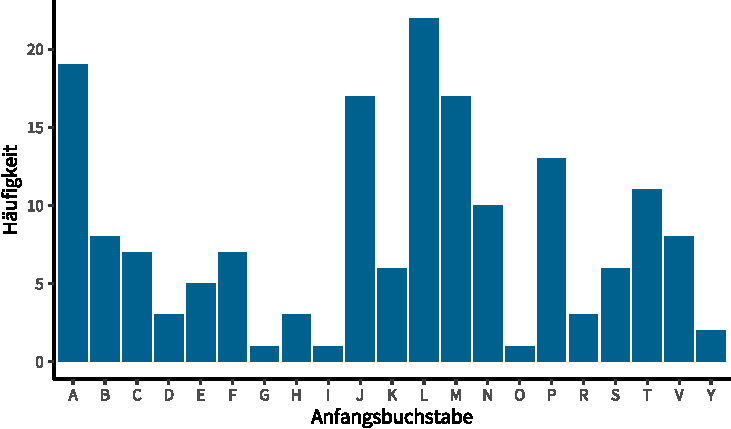
\includegraphics[width=.6\linewidth]{Skript_Statistik_2021_files/figure-latex/stab-1} 

}

\caption{Stabdiagramm}\label{fig:stab}
\end{figure}

\hypertarget{quantitative-variablen-1}{%
\subsection{Quantitative Variablen}\label{quantitative-variablen-1}}

Das oben beschriebene Verfahren funktioniert gut für qualitative Variablen (und diskrete Variablen mit wenigen unterschiedlichen Werten). Für quantitative Variablen wird ein anderes Verfahren empfohlen.

Zur Veranschaulichung soll diese geordnete Liste von Messwerten des Stammdurchmessers von Schwarzkirschen (Beispieldatensatz \texttt{trees} aus \protect\hyperlink{ref-r}{R Core Team 2018}) dienen:

\texttt{8,3\ \ 8,6\ \ 8,8\ 10,5\ 10,7\ 10,8\ 11,0\ 11,0\ 11,1\ 11,2\ 11,3\ 11,4\ 11,4\ 11,7\ 12,0\ 12,9\ 12,9\ 13,3\ 13,7\ 13,8\ 14,0\ 14,2\ 14,5\ 16,0\ 16,3\ 17,3\ 17,5\ 17,9\ 18,0\ 18,0\ 20,6}

Für solche Verteilungen müssen zuerst Klassen (engl. \emph{bins}) gebildet werden, in denen die Werte dann zusammengefasst werden (s. Tabelle \ref{tab:haeufklass}).

\begin{table}

\caption{\label{tab:haeufklass}Häufigkeitstabelle mit klassierten Werten}
\centering
\begin{tabular}[t]{lrrrr}
\toprule
Durchmesser & Absolute Häufigkeit $f$ & $f_{kum}$ & Relative Häufigkeit & $\%_{kum}$\\
\midrule
über 8 bis 10 Zoll & 3 & 3 & 9,7\% & 9,7\%\\
über 10 bis 12 Zoll & 12 & 15 & 38,7\% & 48,4\%\\
über 12 bis 14 Zoll & 6 & 21 & 19,4\% & 67,7\%\\
über 14 bis 16 Zoll & 3 & 24 & 9,7\% & 77,4\%\\
über 16 bis 18 Zoll & 6 & 30 & 19,4\% & 96,8\%\\
über 18 bis 20 Zoll & 0 & 30 & 0\% & 96,8\%\\
über 20 bis 22 Zoll & 1 & 31 & 3,2\% & 100\%\\
\bottomrule
\end{tabular}
\end{table}

Für die Wahl der Klassengrenzen gibt es zwei feste Regeln:

\begin{itemize}
\tightlist
\item
  Alle Werte müssen abgedeckt sein.
\item
  Die Klassen dürfen sich nicht überlappen.
\end{itemize}

Zusätzlich sollten die folgenden Konventionen nach Möglichkeit befolgt werden:

\begin{itemize}
\tightlist
\item
  Klassen sollten gleich große Wertebereiche abdecken.
\item
  Alle Klassen sollten besetzt sein.
\item
  Klassengrenzen sollten möglichst glatte Zahlen sein.
\item
  Aus Gründen der Übersichtlichkeit sollten nicht mehr als 20 Klassen gewählt werden.
\item
  Klassengrenzen sollten \enquote{Klumpen} mit ähnlichen Werten nicht trennen.
\end{itemize}

Die Darstellung erfolgt in so genannten Histogrammen (engl. \emph{histogram}). Abbildung \ref{fig:hist} enthält ein Beispiel für ein Histogramm.

\begin{rtip}
In R können Histogramme mit \verb|hist()| erstellt werden.
\end{rtip}

\begin{figure}[!h]

{\centering 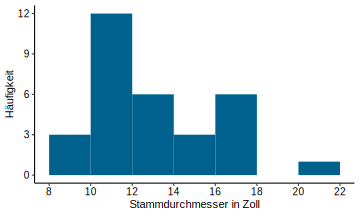
\includegraphics[width=.6\linewidth]{Skript_Statistik_2021_files/figure-latex/hist-1} 

}

\caption{Histogramm}\label{fig:hist}
\end{figure}

\hypertarget{polygone}{%
\subsection{Polygone}\label{polygone}}

Statt ausgefüllten Flächen wie im Histogramm lassen sich für die Häufigkeiten auch Punkte setzen, die dann mit Linien verbunden werden. So entsteht ein Häufigkeitspolygon (s. Abbildung \ref{fig:poly}).

\begin{figure}[!h]

{\centering 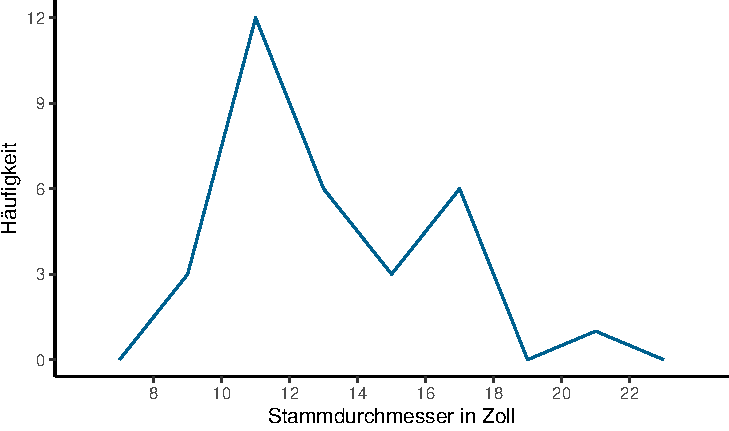
\includegraphics[width=.6\linewidth]{Skript_Statistik_2021_files/figure-latex/poly-1} 

}

\caption{Polygonzug}\label{fig:poly}
\end{figure}

\hypertarget{eigenschaften-von-huxe4ufigkeitsverteilungen}{%
\subsection{Eigenschaften von Häufigkeitsverteilungen}\label{eigenschaften-von-huxe4ufigkeitsverteilungen}}

Polygone von Häufigkeitsverteilungen (insbesondere in geglätteter Form) ergeben Annäherungen an so gennannte Dichtefunktionen (engl. \emph{density functions}). Diese lassen sich mit Attributen (uni-/bimodal, schmal-/breitgipflig, etc.) beschreiben, wie in Abbildung \ref{fig:shapes} veranschaulicht.

\begin{figure}[!h]

{\centering 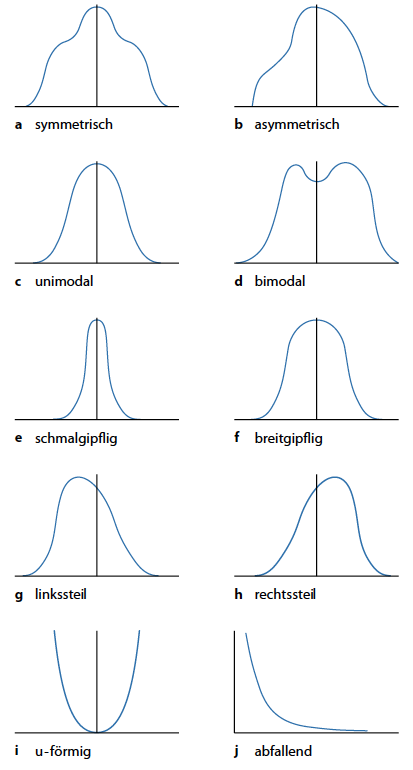
\includegraphics[width=.6\linewidth]{img/shapes} 

}

\caption{Merkmale von Verteilungen [aus: @bortz: 42]}\label{fig:shapes}
\end{figure}

\hypertarget{tipps-zur-vertiefung}{%
\section*{Tipps zur Vertiefung}\label{tipps-zur-vertiefung}}
\addcontentsline{toc}{section}{Tipps zur Vertiefung}

\hypertarget{grundbegriffe}{%
\subsection{Grundbegriffe}\label{grundbegriffe}}

\begin{itemize}
\tightlist
\item
  YouTube-Kanal \enquote{Kurzes Tutorium Statistik}: \href{https://www.youtube.com/watch?v=bJsBcLjke3Q}{Statistische Grundbegriffe}
\item
  Kapitel 1.1 in \protect\hyperlink{ref-bortz}{Bortz und Schuster} (\protect\hyperlink{ref-bortz}{2010})
\item
  Kapitel 1.1 in \protect\hyperlink{ref-benninghaus}{Benninghaus} (\protect\hyperlink{ref-benninghaus}{2007})
\item
  Kapitel 2.1 in \protect\hyperlink{ref-bahrenberg}{Bahrenberg, Giese und Nipper} (\protect\hyperlink{ref-bahrenberg}{2010})
\item
  \emph{Englisch:} Kapitel 1 in \protect\hyperlink{ref-burt}{Burt und Barber} (\protect\hyperlink{ref-burt}{1996})
\end{itemize}

\hypertarget{stichproben}{%
\subsection{Stichproben}\label{stichproben}}

\begin{itemize}
\tightlist
\item
  Kapitel 6.1 in \protect\hyperlink{ref-bortz}{Bortz und Schuster} (\protect\hyperlink{ref-bortz}{2010})
\item
  Kapitel 2.5 in \protect\hyperlink{ref-delange}{Lange und Nipper} (\protect\hyperlink{ref-delange}{2018})
\item
  Kapitel 2.3 in \protect\hyperlink{ref-bahrenberg}{Bahrenberg, Giese und Nipper} (\protect\hyperlink{ref-bahrenberg}{2010})
\item
  \emph{Englisch:} Kapitel 1 in \protect\hyperlink{ref-burt}{Burt und Barber} (\protect\hyperlink{ref-burt}{1996})
\end{itemize}

\hypertarget{skalenniveaus-1}{%
\subsection{Skalenniveaus}\label{skalenniveaus-1}}

\begin{itemize}
\tightlist
\item
  Kapitel 1.2 in \protect\hyperlink{ref-bortz}{Bortz und Schuster} (\protect\hyperlink{ref-bortz}{2010})
\item
  Kapitel 2.5 in \protect\hyperlink{ref-delange}{Lange und Nipper} (\protect\hyperlink{ref-delange}{2018})
\item
  Kapitel 2.1 in \protect\hyperlink{ref-benninghaus}{Benninghaus} (\protect\hyperlink{ref-benninghaus}{2007})
\item
  Kapitel 2.2 in \protect\hyperlink{ref-bahrenberg}{Bahrenberg, Giese und Nipper} (\protect\hyperlink{ref-bahrenberg}{2010})
\item
  YouTube-Kanal \enquote{Kurzes Tutorium Statistik}: \href{https://www.youtube.com/watch?v=TV4tTtW4UBU}{Skalenniveaus}
\item
  \emph{Englisch:} Kapitel 1.3 in \protect\hyperlink{ref-burt}{Burt und Barber} (\protect\hyperlink{ref-burt}{1996})
\end{itemize}

\hypertarget{huxe4ufigkeiten-und-diagramme}{%
\subsection{Häufigkeiten und Diagramme}\label{huxe4ufigkeiten-und-diagramme}}

\begin{itemize}
\tightlist
\item
  YouTube-Kanal \enquote{Kurzes Tutorium Statistik}: \href{https://www.youtube.com/watch?v=LkOBRWXnTRQ}{Stabdiagramme und Histogramme}
\item
  Kapitel 3.1 und 3.2 in \protect\hyperlink{ref-bortz}{Bortz und Schuster} (\protect\hyperlink{ref-bortz}{2010})
\item
  Kapitel 2.5 in \protect\hyperlink{ref-delange}{Lange und Nipper} (\protect\hyperlink{ref-delange}{2018})
\item
  Kapitel 1.2 in \protect\hyperlink{ref-benninghaus}{Benninghaus} (\protect\hyperlink{ref-benninghaus}{2007})
\item
  Kapitel 4.1 in \protect\hyperlink{ref-bahrenberg}{Bahrenberg, Giese und Nipper} (\protect\hyperlink{ref-bahrenberg}{2010})
\item
  \emph{Englisch:} Kapitel 2.1 in \protect\hyperlink{ref-burt}{Burt und Barber} (\protect\hyperlink{ref-burt}{1996})
\end{itemize}

\hypertarget{uxfcbungsaufgaben}{%
\section*{Übungsaufgaben}\label{uxfcbungsaufgaben}}
\addcontentsline{toc}{section}{Übungsaufgaben}

\hypertarget{aufgabe-1-1}{%
\subsection{Aufgabe~1-1}\label{aufgabe-1-1}}

\protect\hyperlink{loesung-1-1}{zur~Lösung}

Teilen Sie in Ihrer Kleingruppe folgende Begriffe untereinander auf:

\begin{itemize}
\tightlist
\item
  Variable
\item
  Kennwert
\item
  Wert
\item
  Grundgesamtheit
\item
  Stichprobe
\item
  Untersuchungselement
\end{itemize}

Gehen Sie nun für jeden Begriff wie folgt vor:

\begin{enumerate}
\def\labelenumi{\arabic{enumi}.}
\tightlist
\item
  Erklären Sie der Reihe nach \enquote{Ihren} Begriff den anderen Gruppenmitgliedern, gerne auch mit Beispielen.
\item
  Die anderen Gruppenmitglieder nehmen die Rolle von unwissenden Dritten ein und stellen bei Bedarf Nachfragen.
\item
  Die anderen Gruppenmitglieder geben direkt danach Feedback auf die Erklärung:

  \begin{itemize}
  \tightlist
  \item
    Was fanden Sie gut erklärt?
  \item
    Was fanden Sie unverständlich?
  \item
    Was hat Ihnen gefehlt?
  \end{itemize}
\end{enumerate}

\hypertarget{aufgabe-1-2}{%
\subsection{Aufgabe~1-2}\label{aufgabe-1-2}}

\protect\hyperlink{loesung-1-2}{zur~Lösung}

Finden Sie als Gruppe jeweils zwei Beispiele für:

\begin{itemize}
\tightlist
\item
  systematische Zufallsstichproben
\item
  geschichtete Zufallsstichproben
\item
  Klumpenstichproben
\end{itemize}

\hypertarget{aufgabe-1-3}{%
\subsection{Aufgabe~1-3}\label{aufgabe-1-3}}

\protect\hyperlink{loesung-1-3}{zur~Lösung}

Bestimmen Sie das Skalenniveau der folgenden Variablen. Kennzeichnen Sie darüber hinaus, ob die Variable qualitativ, diskret oder stetig ist.

\begin{enumerate}
\def\labelenumi{\alph{enumi})}
\tightlist
\item
  Lebensalter in Jahren
\item
  Regenmenge in mm
\item
  Güteklasse
\item
  Passagieraufkommen
\item
  Baujahr
\item
  Geschwindigkeit in km/h
\item
  Sozialstatus (Unter-, Mittel und Oberschicht)
\item
  Temperatur in °F
\item
  Fläche eines Bundeslands in km²
\item
  Temperatur in K
\item
  Einwohnerzahl
\item
  Pegelstand
\item
  Staatsangehörigkeit
\item
  Interesse an Statistik (gering bis hoch)
\item
  Klausurnote
\item
  Bodentyp
\item
  Entfernung zum Stadtzentrum in km
\item
  Körpergröße
\item
  Kleidergröße (S bis XXL)
\item
  Monatliches Nettoeinkommen
\end{enumerate}

\hypertarget{aufgabe-1-4}{%
\subsection{Aufgabe~1-4}\label{aufgabe-1-4}}

\protect\hyperlink{loesung-1-4}{zur~Lösung}

Folgende Werte seien erfasst über die Lebensdauer von Klimaanlagen in Stunden (Beispieldatensatz \texttt{aircondit7} aus \protect\hyperlink{ref-r}{R Core Team 2018}):

\begin{verbatim}
14 23 15 139 13 39 188 22 50 3 36 46 30 5 102 5 88 22 197 72 210 97 79 44
\end{verbatim}

\begin{enumerate}
\def\labelenumi{\alph{enumi})}
\tightlist
\item
  Erstellen Sie eine Häufigkeitstabelle. Welche Klassen wählen Sie und warum?
\item
  Zeichnen Sie ein Histogramm.
\item
  Beschreiben Sie die Verteilung.
\end{enumerate}

\hypertarget{aufgabe-1-5}{%
\subsection{Aufgabe~1-5}\label{aufgabe-1-5}}

\protect\hyperlink{loesung-1-5}{zur~Lösung}

Sind die folgenden Aussagen wahr oder unwahr?

\begin{enumerate}
\def\labelenumi{\alph{enumi})}
\tightlist
\item
  Die Auswahl z. B. jedes 100. Merkmalsträgers nennt man „systematische Stichprobe``.
\item
  Eine Stichprobe kann eine Grundgesamtheit niemals völlig richtig repräsentieren, es gibt immer einen Zufallsfehler.
\item
  Die Größe der Stichprobe wird auch mit \(N\) bezeichnet.
\item
  Klassengrenzen müssen so gewählt werden, dass alle Werte abgedeckt sind.
\item
  Je stärker die Werte der Variablen streuen, desto kleiner sollte die Stichprobe sein.
\item
  Variablen auf der Verhältnisskala sind immer metrisch und stetig.
\item
  Verhältnisskala und Intervallskala unterscheiden sich durch den natürlichen Nullpunkt.
\item
  Intervallskalierte Daten können immer auf die Nominalskala transformiert werden.
\item
  Ordinalskalierte Daten können immer auf die Intervallskala transformiert werden.
\item
  Eine stetige Variable ist nicht zwingend auch metrisch.
\item
  Im Gegensatz zu nominalskalierten Variablen lassen sich Werte von ordinalskalierten Variablen in eine sinnvolle Reihenfolge bringen.
\item
  Die relative Häufigkeit eines Werts ist nie größer als 100\%.
\item
  Verfahren der deskriptiven Statistik sind immer auch univariat.
\item
  Klassengrenzen dürfen sich in Ausnahmefällen überlappen.
\item
  \(x_3\) ist immer kleiner als \(x_4\).
\item
  Variablen auf der Verhältnisskala haben einen natürlichen Nullpunkt.
\item
  Die absolute Häufigkeit eines Werts ist immer eine positive ganze Zahl.
\item
  Wenn man die Urliste ordnet, erhält man die geordnete Liste.
\end{enumerate}

\hypertarget{mauxdfzahlen}{%
\chapter{Maßzahlen}\label{mauxdfzahlen}}

\hypertarget{lernziele-dieser-sitzung-1}{%
\subsection*{Lernziele dieser Sitzung}\label{lernziele-dieser-sitzung-1}}
\addcontentsline{toc}{subsection}{Lernziele dieser Sitzung}

Sie können\ldots{}

\begin{itemize}
\tightlist
\item
  die wichtigsten Lagemaße von Stichproben bestimmen.
\item
  die wichtigsten Streumaße von Stichproben bestimmen.
\item
  Boxplots interpretieren.
\end{itemize}

\hypertarget{lehrvideos-sommersemester-2020-1}{%
\subsection*{Lehrvideos (Sommersemester 2020)}\label{lehrvideos-sommersemester-2020-1}}
\addcontentsline{toc}{subsection}{Lehrvideos (Sommersemester 2020)}

\begin{itemize}
\tightlist
\item
  \href{https://video01.uni-frankfurt.de/Mediasite/Play/bbb30f8025cf48e99a48700b0600e1e11d}{2a) Lagemaße}
\item
  \href{https://video01.uni-frankfurt.de/Mediasite/Play/cfdb254c058f44228e7b026f36986cc31d}{2b) Streumaße}
\item
  \href{https://video01.uni-frankfurt.de/Mediasite/Play/d115769da4ee4e25a9062a9b2e2e11c41d}{2c) Klassierte Verteilungen}

  \begin{itemize}
  \tightlist
  \item
    In diesem Video ist mir ein Fehler unterlaufen: Bei Minute 6:30 muss das arithmetische Mittel \(\bar{x}\approx4{,}59\) betragen. Daraus ergibt sich ein Folgefehler: Die Varianz müsste den Wert \(s^2\approx14{,}56\) haben.
  \end{itemize}
\end{itemize}

\hypertarget{einleitende-bemerkungen}{%
\section{Einleitende Bemerkungen}\label{einleitende-bemerkungen}}

Die im Folgenden besprochenen Maßzahlen (oder Kennzahlen, Parameter) verdichten (oder aggregieren) Häufigkeitsverteilungen einer Variable. Durch diese Parameter kann das Charakteristische einer Verteilung schnell erfasst und vergleichbar gemacht werden. Die Verdichtung auf Maßzahlen geht jedoch immer auch mit Informationsverlust einher.

Die Möglichkeit der Angabe statistischer Maßzahlen ist abhängig vom Skalenniveau der Daten, wie der Überblick in Tabelle \ref{tab:mass} zeigt.

\begin{table}

\caption{\label{tab:mass}Die wichtigsten Maßzahlen}
\centering
\begin{tabular}[t]{llll}
\toprule
Parameter & Typ & Mindestes Skalenniveau & Formel\\
\midrule
Modalwert & Lagemaß & nominal & \medskip$\mathit{Mo}$\\
Median & Lagemaß & ordinal & \medskip$\def\arraystretch{1.2} \mathit{Md} = \Bigg\{\begin{array}{@{}c@{}}\frac{x_{(\frac{n}{2})}+x_{(\frac{n}{2}+1)}}{2} \quad \textrm{falls }n \textrm{ gerade}\\[6pt] x_{(\frac{n+1}{2})}\quad \textrm{falls }n \textrm{ ungerade}\end{array}$\\
Arithmetisches Mittel & Lagemaß & metrisch & \medskip$\bar{x}=\frac{\sum\limits_{i=1}^{n}x _{i}}{n}$\\
Spannweite & Streumaß & ordinal & \medskip$R=x_{(n)}-x_{(1)}$\\
Quartilsabstand & Streumaß & ordinal & \medskip$\mathit{IQR}=Q_3-Q_1$\\
Varianz & Streumaß & metrisch & \medskip$s^2=\frac{\sum\limits_{i=1}^{n}(x_{i}-\bar{x})^2}{n-1}$\\
Standardabweichung & Streumaß & metrisch & \medskip$s=\sqrt{s^2}$\\
\bottomrule
\end{tabular}
\end{table}

\hypertarget{beispielverteilung}{%
\subsection{Beispielverteilung}\label{beispielverteilung}}

Alle Berechnungen von Maßzahlen werden am folgenden Beispiel illustriert: Für die 14 Gemeinden im Landkreis Rothenberge wurde die jeweilige Anzahl an Gaststätten erhoben. Die Zählung ergab die Wertereihe in Tabelle \ref{tab:werte}.

\begin{table}

\caption{\label{tab:werte}Beispielverteilung}
\centering
\begin{tabular}[t]{rrrrrrrrrrrrrr}
\toprule
$x_{1}$ & $x_{2}$ & $x_{3}$ & $x_{4}$ & $x_{5}$ & $x_{6}$ & $x_{7}$ & $x_{8}$ & $x_{9}$ & $x_{10}$ & $x_{11}$ & $x_{12}$ & $x_{13}$ & $x_{14}$\\
\midrule
4 & 1 & 4 & 1 & 5 & 5 & 0 & 1 & 8 & 5 & 1 & 25 & 3 & 3\\
\bottomrule
\end{tabular}
\end{table}

\hypertarget{lagemauxdfe}{%
\section{Lagemaße}\label{lagemauxdfe}}

Lagemaße (auch Maße der Zentraltendenz, Lokalisationsparameter, Mittelwerte, engl. \emph{measures of central tendency}) bezeichnen alle statistischen Maßzahlen, die eine Verteilung repräsentieren, indem sie die Lage der mittleren oder häufigsten Variablenwerte angeben.

Im Falle einer unimodalen, perfekt symmetrischen Verteilung (z.~B. Glockenform) haben alle drei Lageparameter den gleichen Wert. Je weiter Verteilungen von dieser Form abweichen -- durch Mehrgipfligkeit oder Asymmetrie -- desto unpräziser ist die Beschreibung der Verteilung durch einen einzigen Parameter.

\hypertarget{median}{%
\subsection{Median}\label{median}}

Der Median (engl. \emph{median}) einer Verteilung ist der Wert, der größer als genau 50\% aller Werte ist.

Da dies eine Größer-kleiner-Relation der Werte voraussetzt, kann der Median nur für ordinale und metrische Skalenniveaus angegeben werden.

Im Folgenden wird die (einfachere) Bestimmung des Medians nach \protect\hyperlink{ref-bortz}{Bortz und Schuster} (\protect\hyperlink{ref-bortz}{2010}) verwendet. \protect\hyperlink{ref-benninghaus}{Benninghaus} (\protect\hyperlink{ref-benninghaus}{2007}) beschreibt ein anderes Verfahren, welches zu anderen Ergebnissen kommen kann.

Um den Median zu bestimmen, wird zunächst eine geordnete Liste angefertigt, indem die Werte aufsteigend sortiert werden. Diese sortierten Werte werden mit \(x_{(1)}, x_{(2)}, x_{(3)}, ..., x_{(n)}\) bezeichnet (also mit Klammern). Für unsere Beispielverteilung ergibt sich Tabelle \ref{tab:sort}.

\begin{table}

\caption{\label{tab:sort}Sortierte Wertereihe}
\centering
\begin{tabular}[t]{rrrrrrrrrrrrrr}
\toprule
$x_{(1)}$ & $x_{(2)}$ & $x_{(3)}$ & $x_{(4)}$ & $x_{(5)}$ & $x_{(6)}$ & $x_{(7)}$ & $x_{(8)}$ & $x_{(9)}$ & $x_{(10)}$ & $x_{(11)}$ & $x_{(12)}$ & $x_{(13)}$ & $x_{(14)}$\\
\midrule
0 & 1 & 1 & 1 & 1 & 3 & 3 & 4 & 4 & 5 & 5 & 5 & 8 & 25\\
\bottomrule
\end{tabular}
\end{table}

Bei einer ungeraden Stichprobengröße \(n\) teilt der \((\frac{n+1}{2})\)-te Wert (also der Wert genau in der Mitte) die Stichprobe in zwei Hälften, weshalb gilt:

\[
  \mathit{Md} = x_{(\frac{n+1}{2})} \quad \text{falls }n\text{ ungerade.}
  \label{eq:med1}
\]

Bei geradem \(n\) entstehen zwei gleich große Hälften der Stichprobe: \(x_{(1)}\) bis \(x_{(\frac{n}{2})}\) einerseits, und \(x_{(\frac{n}{2}+1)}\) bis \(x_{(n)}\) andererseits. Der Durchschnitt zwischen \(x_{(\frac{n}{2})}\) und \(x_{(\frac{n}{2}+1)}\) teilt die Stichprobe in zwei Hälften. Es gilt:

\[
  \mathit{Md} = \frac{x_{(\frac{n}{2})} + x_{(\frac{n}{2}+1)}}{2} \quad \text{falls } n \text{ gerade.}
  \label{eq:med2}
\]

In unserem Beispiel ist \(n=14\) und damit gerade. Der Median errechnet also nach Formel \eqref{eq:med2} wie folgt:

\[
  \begin{aligned}
    \mathit{Md} & = \frac{x_{(7)} + x_{(8)}}{2} \\[4pt]
                & = \frac{3 + 4}{2} \\[4pt]
                & = 3{,}5
  \end{aligned}
\]

\begin{rtip}
In R gibt die Funktion \verb|median()| den Median einer Verteilung aus.
\end{rtip}

\hypertarget{modalwert}{%
\subsection{Modalwert}\label{modalwert}}

Der Modalwert \(\mathit{Mo}\) (auch Modus, engl. \emph{mode}) gibt den häufigsten Wert oder die häufigsten Werte einer Verteilung an.

Der Modalwert kann so auch (als einziger Mittelwert) für nominalskalierte Variablen angegeben werden.

Bei ordinalen und metrischen Skalenniveaus sind folgende Besonderheiten zu beachten:

\begin{itemize}
\tightlist
\item
  Wird der Modus einer Verteilung durch unmittelbar benachbarte Werte gebildet, wird er als Kombination (bei metrischen Variablen als arithmetisches Mittel) dieser Werte angegeben.
\item
  Bei bimodalen (multimodalen) Verteilungen werden beide (alle) Modalwerte angegeben.
\end{itemize}

Hierzu müssen die Häufigkeiten der Werte bekannt sein, bzw. bestimmt werden (s. Tabelle \ref{tab:mod}).

\begin{table}

\caption{\label{tab:mod}Häufigkeiten der Beispielverteilung}
\centering
\begin{tabular}[t]{rr}
\toprule
Wert $x_i$ & Häufigkeit $f_i$\\
\midrule
0 & 1\\
1 & 4\\
3 & 2\\
4 & 2\\
5 & 3\\
8 & 1\\
25 & 1\\
\bottomrule
\end{tabular}
\end{table}

Der Modalwert der Beispielverteilung beträgt 1, da der Wert 1 am häufigsten (viermal) vorkommt.

\hypertarget{arithmetisches-mittel}{%
\subsection{Arithmetisches Mittel}\label{arithmetisches-mittel}}

Das arithmetische Mittel (auch Mittelwert, Durchschnitt, engl. \emph{mean}) ist das gebräuchlichste Lagemaß und Grundlage für viele statistische Verfahren.

Das arithmetische Mittel setzt ein metrisches Skalenniveau voraus.

Die Berechnung des arithmetischen Mittels einer Stichprobe erfolgt durch die Formel:

\[
 \bar{x}=\frac{\sum\limits _{i=1}^{n}x_{i}}{n}
 \label{eq:am}
\]

Für unsere Beispielverteilung ergibt sich durch einsetzen in Formel \eqref{eq:am}:
\[
  \begin{aligned}
     \bar{x}&=\frac{\sum\limits _{i=1}^{14}x_{i}}{14} \\[4pt]
            &=\frac{4+1+4+1+5+5+0+1+8+5+1+25+3+3}{14} \\[4pt]
            &=\frac{63}{14}\\[4pt]
            &\approx 4{,}71
  \end{aligned}
\]

\begin{rtip}
Der Befehl für die Ermittlung des arithmetischen Mittels in R lautet \verb|mean()|.
\end{rtip}

\hypertarget{streumauxdfe}{%
\section{Streumaße}\label{streumauxdfe}}

Streumaße (auch Streuungs-, Variabilitäts-, Dispersionswerte, engl. \emph{measures of variability}) geben Auskunft darüber, wie heterogen die Werte einer Verteilung sind, d.~h. wie breit sie gestreut sind. Während Lagemaße den typischen Wert einer Verteilung ermitteln, zeigen Streumaße, wie gut (oder eigentlich: wie schlecht) dieser typische Wert die Verteilung repräsentiert.

\hypertarget{spannweite}{%
\subsection{Spannweite}\label{spannweite}}

Die Spannweite (engl. \emph{range}) gibt Auskunft darüber, wie groß der Wertebereich ist, der von einer Verteilung abgedeckt wird. Sie wird (für metrische Skalen) als die Differenz vom größten zum kleinsten Wert (also vom letzten zum ersten Wert einer geordneten Werteliste) angegeben:

\[
 R=x_{(n)} - x_{(1)}
 \label{eq:range}
\]

Für unsere Beispielstichprobe ergibt sich (mit Blick auf Tabelle \ref{tab:sort}):

\nopagebreak

\[
  \begin{aligned}
     R&=x_{(14)} - x_{(1)} \\[4pt]
     &=25-0 \\[4pt]
     &=25
  \end{aligned}
\]

\begin{rtip}
In R gibt die Funktion \verb|range()| die Werte für $x_{(1)}$ und $x_{(n)}$ aus.
\end{rtip}

\hypertarget{quartilsabstand}{%
\subsection{Quartilsabstand}\label{quartilsabstand}}

Der Quartilsabstand (auch Interquartilsabstand, engl. \emph{interquartile range, IQR}) gibt die Größe des Wertebereichs der mittleren 50\% einer Verteilung an.

Genau so wie der Median eine Messwertreihe in zwei gleich große Hälften \enquote{schneidet}, schneiden die Quartile die Werte in Viertel. Dabei liegt der so genannte untere Angelpunkt \(Q_1\) genau über 25\% der Werte, \(Q_2\) ist identisch mit dem Median und der obere Angelpunkt \(Q_3\) liegt genau über 75\% der Werte.

Der Angelpunkt \(Q_1\) wird ermittelt, indem der Median für die unteren 50\% (\(Q_3\): die oberen 50\%) der Werte bestimmt wird -- also jener Werte, die theoretisch unterhalb des Medians der Gesamtverteilung liegen.

Dabei folgen wir \protect\hyperlink{ref-bortz}{Bortz und Schuster} (\protect\hyperlink{ref-bortz}{2010}) und nehmen im Fall eines ungeraden \(n\) den Median auf beiden Seiten hinzu.

Die Formel für den Quartilsabstand lautet:

\[
  \begin{aligned}
    \mathit{IQR}=Q_3-Q_1
  \end{aligned}
  \label{eq:iqr}
\]

Der Quartilsabstand ist Ausreißern gegenüber stabiler als die Spannweite, da extreme hohe oder niedrige Wert nicht in die Berechnung einfließen.

In unserem Beispiel (mit \(n=14\)) ist die untere Hälfte der Verteilung:

\begin{table}[H]
\centering
\begin{tabular}{rrrrrrr}
\toprule
$x_{(1)}$ & $x_{(2)}$ & $x_{(3)}$ & $x_{(4)}$ & $x_{(5)}$ & $x_{(6)}$ & $x_{(7)}$\\
\midrule
0 & 1 & 1 & 1 & 1 & 3 & 3\\
\bottomrule
\end{tabular}
\end{table}

\(Q_1\) ist der Median dieser Werte, also \(x_{(4)}=1\).

Die oberen 7 Werte lauten:

\begin{table}[H]
\centering
\begin{tabular}{rrrrrrr}
\toprule
$x_{(8)}$ & $x_{(9)}$ & $x_{(10)}$ & $x_{(11)}$ & $x_{(12)}$ & $x_{(13)}$ & $x_{(14)}$\\
\midrule
4 & 4 & 5 & 5 & 5 & 8 & 25\\
\bottomrule
\end{tabular}
\end{table}

\(Q_3\) ist also \(x_{(11)} = 5\).

Für den Quartilsabstand ergibt sich durch einsetzen in Formel \eqref{eq:iqr}:

\[
  \begin{aligned}
    \mathit{IQR}&=5-1 \\[4pt]
       &=4 \\[4pt]
  \end{aligned}
\]

\begin{rtip}
In R werden die Quartile üblicherweise mit \verb|quantile()| und der Quartilsabstand mit \verb|IQR()| bestimmt.
\end{rtip}

\textbf{Achtung:} Genau wie für den Median gibt es auch für die Ermittlung der Quartile bzw. des Quartilsabstands unterschiedliche Verfahren. Die Ergebnisse dieser R-Funktionen weichen hier deshalb meist leicht vom hier besprochenen Verfahren ab!

\hypertarget{varianz}{%
\subsection{Varianz}\label{varianz}}

Die Varianz einer Messwertreihe (engl. \emph{variance}) kann verstanden werden als der durchschnittliche quadrierte Abstand der Werte zum arithmetischen Mittel.

Die Formel lautet:

\[
  s^2=\frac{\sum\limits_{i=1}^{n}(x_{i}-\bar{x})^2}{n-1}
  \label{eq:var}
\]

Die Quadrierung der Differenz hat dabei einen doppelten Effekt: Zum einen bekommen auch negative Differenzen ein positives Vorzeichen, so dass sich positive und negative Differenzen nicht neutralisieren. Zum anderen werden hierdurch besonders große Abweichungen zum arithmetischen Mittel stärker gewichtet als dies ohne Quadrierung der Fall wäre.

Zudem fällt auf, dass im Gegensatz zur Formel für das arithmetische Mittel im Nenner \(n-1\) steht und nicht etwa \(n\). Dies hat mit so genannten Freiheitsgraden zu tun, die wir allerdings erst in \protect\hyperlink{freiheitsgrade}{Sitzung 5} genauer kennenlernen.

Für unsere Beispielstichprobe wird die Berechnung für alle einzelnen \((x_i-\bar{x})^2\) schnell aufwendig und unübersichtlich. Deshalb berechnen wir ihre Summe hier mit Hilfe einer Häufigkeitstabelle (s. Tabelle \ref{tab:freq}). Dabei werden alle distinkten Werte einzeln transformiert und in der letzten Spalte mit ihrer Häufigkeit multipliziert.

\begin{table}

\caption{\label{tab:freq}Häufigkeitstabelle zur Berechnung der Varianz}
\centering
\begin{tabular}[t]{rrrrr}
\toprule
Werte $x_i$ & Häufigk. $f_i$ & $(x_i- \bar{x})$ & $(x_i- \bar{x})^2$ & $f_i\cdot(x_i -\bar{x})^2$\\
\midrule
0 & 1 & -4,71 & 22,18 & 22,18\\
1 & 4 & -3,71 & 13,76 & 55,04\\
3 & 2 & -1,71 & 2,92 & 5,84\\
4 & 2 & -0,71 & 0,50 & 1,00\\
5 & 3 & 0,29 & 0,08 & 0,24\\
8 & 1 & 3,29 & 10,82 & 10,82\\
25 & 1 & 20,29 & 411,68 & 411,68\\
\bottomrule
\end{tabular}
\end{table}

Schließlich werden die Werte in Formel \eqref{eq:var} eingesetzt:

\nopagebreak

\[\begin{aligned}
    s^2&=\frac{\sum\limits_{i=1}^{14}(x_{i}-\bar{x})^2}{14-1} \\[4pt]
       &\approx\frac{22{,}18+55{,}04+5{,}84+1+0{,}24+10{,}82+411{,}68}{13} \\[4pt]
       &=\frac{506{,}80}{13}\\[4pt]
       &\approx 38{,}98
\end{aligned}\]

Eine solche Tabelle lässt sich analog auch für die Berechnung von Summen größerer Messwertreihen für das arithmetische Mittel verwenden.

Zudem lässt dieses Verfahren sich auf klassierte Daten anwenden, wenn für \(x_i\) der Mittelwert der Klassen eingesetzt wird (womit allerdings Informations- und Präzisionsverlust einhergeht).

\begin{rtip}
In R lautet der Befehl für die Errechnung der Varianz \verb|var()|.
\end{rtip}

\hypertarget{standardabweichung}{%
\subsection{Standardabweichung}\label{standardabweichung}}

Die Standardabweichung (engl. \emph{standard deviation}) ist das gebräuchlichste Streumaß und spielt eine herausragende Rolle in den allermeisten statistischen Verfahren.

Die Standardabweichung einer Messwertreihe ist definiert als die Quadratwurzel ihrer Varianz:

\[
  \begin{aligned}
    s=\sqrt{s^2}
  \end{aligned}
  \label{eq:sd}
\]

Indem hier die Wurzel gezogen wird, wird in gewisser Weise die Quadrierung der Differenzen für die Varianz wieder \enquote{korrigiert}. Insbesondere wird die Quadrierung der Maßeinheit wieder aufgehoben -- die Standardabweichung hat also die gleiche Einheit wie die Messreihe selbst.

In unserem Beispiel beträgt die Standardabweichung also:

\[
  \begin{aligned}
    s&\approx\sqrt{38{,}98}
      \approx6{,}24
  \end{aligned}
\]

\begin{rtip}
Die Standardabweichung wird in R mit der Funktion \verb|sd()| berechnet.
\end{rtip}

\hypertarget{boxplot}{%
\section{Boxplot}\label{boxplot}}

Der Boxplot (auch Box-and-whisker-plot) kombiniert einige der gebräuchlichsten Maßzahlen in einer übersichtlichen Grafik (s. Abbildung \ref{fig:box}).

\begin{figure}[!h]

{\centering 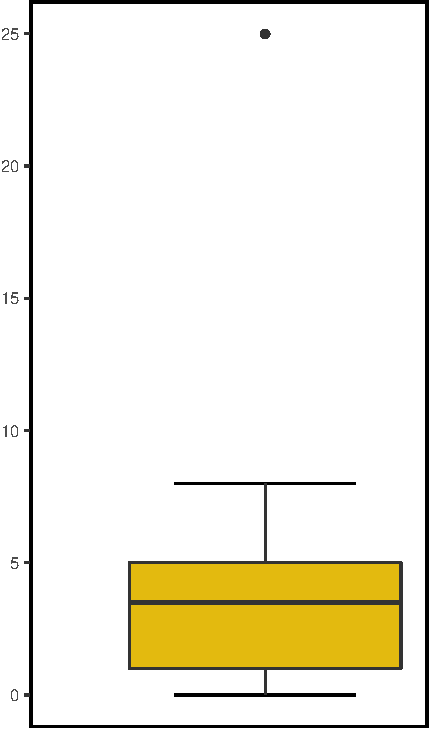
\includegraphics[width=0.35\linewidth]{Skript_Statistik_2021_files/figure-latex/box-1} 

}

\caption{Boxplot der Beispielverteilung}\label{fig:box}
\end{figure}

Die Höhe der \enquote{Box} definiert sich durch den Quartilsabstand, der mittlere Strich markiert den Median und die \enquote{Whisker} markieren den Wertebereich insgesamt -- wobei Ausreißer, deren Abstand zur Box mehr als das 1,5-Fache des Quartilsabstands beträgt, üblicherweise gar nicht oder (wie hier) gesondert mit Punkten markiert werden.

\begin{rtip}
In R lässt sich ein Boxplot mit dem Befehl \verb|boxplot()| ausgeben.
\end{rtip}

\hypertarget{tipps-zur-vertiefung-1}{%
\section*{Tipps zur Vertiefung}\label{tipps-zur-vertiefung-1}}
\addcontentsline{toc}{section}{Tipps zur Vertiefung}

\hypertarget{lagemauxdfe-1}{%
\subsection{Lagemaße}\label{lagemauxdfe-1}}

\begin{itemize}
\tightlist
\item
  Kapitel 2.1 in \protect\hyperlink{ref-bortz}{Bortz und Schuster} (\protect\hyperlink{ref-bortz}{2010})
\item
  Kapitel 3.3.2 in \protect\hyperlink{ref-delange}{Lange und Nipper} (\protect\hyperlink{ref-delange}{2018})
\item
  Kapitel 3.3.1 in \protect\hyperlink{ref-benninghaus}{Benninghaus} (\protect\hyperlink{ref-benninghaus}{2007})
\item
  Kapitel 4.2.1 in \protect\hyperlink{ref-bahrenberg}{Bahrenberg, Giese und Nipper} (\protect\hyperlink{ref-bahrenberg}{2010})
\item
  YouTube-Kanal \enquote{Kurzes Tutorium Statistik}: \href{https://www.youtube.com/watch?v=Kx9aHOMVPEg}{Arithmetisches, harmonisches und geometrisches Mittel}
\item
  YouTube-Kanal \enquote{Kurzes Tutorium Statistik}: \href{https://www.youtube.com/watch?v=HsDeAoBOyS4}{Boxplots, Median, Quartile}
\item
  \emph{Englisch:} Kapitel 2.2 in \protect\hyperlink{ref-burt}{Burt und Barber} (\protect\hyperlink{ref-burt}{1996})
\end{itemize}

\hypertarget{streumauxdfe-1}{%
\subsection{Streumaße}\label{streumauxdfe-1}}

\begin{itemize}
\tightlist
\item
  Kapitel 2.2 in \protect\hyperlink{ref-bortz}{Bortz und Schuster} (\protect\hyperlink{ref-bortz}{2010})
\item
  Kapitel 3.3.3 in \protect\hyperlink{ref-delange}{Lange und Nipper} (\protect\hyperlink{ref-delange}{2018})
\item
  Kapitel 3.1.2 in \protect\hyperlink{ref-benninghaus}{Benninghaus} (\protect\hyperlink{ref-benninghaus}{2007})
\item
  Kapitel 4.2.2 in \protect\hyperlink{ref-bahrenberg}{Bahrenberg, Giese und Nipper} (\protect\hyperlink{ref-bahrenberg}{2010})
\item
  YouTube-Kanal \enquote{Kurzes Tutorium Statistik}: \href{https://www.youtube.com/watch?v=3oZrS3ZWVcA}{Streumaße - Varianz, Standardabweichung, Variationskoeffizient und mehr!}
\item
  \emph{Englisch:} Kapitel 2.3 in \protect\hyperlink{ref-burt}{Burt und Barber} (\protect\hyperlink{ref-burt}{1996})
\end{itemize}

\hypertarget{boxplot-1}{%
\subsection{Boxplot}\label{boxplot-1}}

\begin{itemize}
\tightlist
\item
  Kapitel 3.4 in \protect\hyperlink{ref-bortz}{Bortz und Schuster} (\protect\hyperlink{ref-bortz}{2010})
\item
  Kapitel 5.3.1 in \protect\hyperlink{ref-delange}{Lange und Nipper} (\protect\hyperlink{ref-delange}{2018})
\item
  YouTube-Kanal \enquote{Kurzes Tutorium Statistik}: \href{https://www.youtube.com/watch?v=HsDeAoBOyS4}{Boxplots, Median, Quartile}
\item
  \emph{Englisch:} Kapitel 16.3 in \protect\hyperlink{ref-burt}{Burt und Barber} (\protect\hyperlink{ref-burt}{1996})
\end{itemize}

\hypertarget{uxfcbungsaufgaben-1}{%
\section*{Übungsaufgaben}\label{uxfcbungsaufgaben-1}}
\addcontentsline{toc}{section}{Übungsaufgaben}

\hypertarget{aufgabe-2-1}{%
\subsection{Aufgabe~2-1}\label{aufgabe-2-1}}

\protect\hyperlink{loesung-2-1}{zur~Lösung}

Berechnen Sie das arithmetische Mittel für die folgenden Verteilungen:

\hypertarget{a}{%
\subsubsection{a)}\label{a}}

\begin{verbatim}
72 55 69 69 30 61
\end{verbatim}

\hypertarget{b}{%
\subsubsection{b)}\label{b}}

\begin{verbatim}
0,759  0,296  0,687  0,7  -0,418  0,459  -0,4  -0,008
\end{verbatim}

\hypertarget{c}{%
\subsubsection{c)}\label{c}}

\begin{verbatim}
951,73  859,29  937,4  939,96  716,45  891,83  719,92  798,38  864,21  670,99
\end{verbatim}

Tauschen Sie sich danach in der Lerngruppe darüber aus \ldots{}

\begin{itemize}
\tightlist
\item
  Was schreiben Sie wann auf?
\item
  Wie geben Sie die Zahlen und Rechenschritte in den Taschenrechner ein?
\item
  Wie überprüfen Sie ggf. Ihr Ergebnis mit Hilfe des Taschenrechners?
\end{itemize}

\hypertarget{aufgabe-2-2}{%
\subsection{Aufgabe~2-2}\label{aufgabe-2-2}}

\protect\hyperlink{loesung-2-2}{zur~Lösung}

Wiederholen Sie Aufgabe 1, aber berechnen Sie statt des arithmetischen Mittels die Standardabweichung (und tauschen sich darüber aus).

\hypertarget{aufgabe-2-3}{%
\subsection{Aufgabe~2-3}\label{aufgabe-2-3}}

\protect\hyperlink{loesung-2-3}{zur~Lösung}

Bei einer Befragung jedes 500. Studierenden im Matrikel einer privaten Hochschule wurden folgende Angaben zur Haushaltsgröße gemacht:

\begin{verbatim}
1 4 4 2 3 2 3 5 2 7 2 1 1
\end{verbatim}

\begin{enumerate}
\def\labelenumi{\alph{enumi})}
\tightlist
\item
  Welches Skalenniveau liegt vor? (\protect\hyperlink{skalenniveaus}{Sitzung 1})
\item
  Berechnen Sie Modalwert,
\item
  Median und
\item
  arithmetisches Mittel der Stichprobe.
\item
  Berechnen Sie außerdem die Spannweite,
\item
  den Quartilsabstand,
\item
  die Varianz und
\item
  die Standardabweichung der Stichprobe.
\item
  Zeichnen Sie einen Boxplot der Stichprobenverteilung.
\end{enumerate}

\hypertarget{aufgabe-2-4}{%
\subsection{Aufgabe~2-4}\label{aufgabe-2-4}}

\protect\hyperlink{loesung-2-4}{zur~Lösung}

Eine Messreihe der Körperlänge weiblicher Beutelratten hat folgende Werte in cm erfasst (Beispieldatensatz \texttt{fossum} aus \protect\hyperlink{ref-daag}{Maindonald und Braun 2015}):

\begin{table}[H]
\centering
\begin{tabular}{lrrrr}
\toprule
$x$ & $k_i$ & $f_i$ & $f_{kum}$ & $f_i \cdot k_i$\\
\midrule
von 75 bis unter 77,5 cm & 76,25 & 1 & 1 & 76,25\\
von 77,5 bis unter 80 cm & 78,75 & 0 & 1 & 0,00\\
von 80 bis unter 82,5 cm & 81,25 & 3 & 4 & 243,75\\
von 82,5 bis unter 85 cm & 83,75 & 5 & 9 & 418,75\\
von 85 bis unter 87,5 cm & 86,25 & 7 & 16 & 603,75\\
von 87,5 bis unter 90 cm & 88,75 & 14 & 30 & 1242,50\\
von 90 bis unter 92,5 cm & 91,25 & 9 & 39 & 821,25\\
von 92,5 bis unter 95 cm & 93,75 & 2 & 41 & 187,50\\
von 95 bis unter 97,5 cm & 96,25 & 2 & 43 & 192,50\\
\bottomrule
\end{tabular}
\end{table}

\begin{enumerate}
\def\labelenumi{\alph{enumi})}
\tightlist
\item
  Wie groß ist der Quartilsabstand?
\item
  Bestimmen Sie das arithmetische Mittel der Reihe.
\item
  Berechnen Sie auch die Varianz und
\item
  die Standardabweichung.
\end{enumerate}

\hypertarget{aufgabe-2-5}{%
\subsection{Aufgabe~2-5}\label{aufgabe-2-5}}

\protect\hyperlink{loesung-2-5}{zur~Lösung}

In Wiesbaum soll ein Kulturzentrum entstehen. Zwei leerstehende Industriegebäude -- eine Ziegelei und ein Möbellager -- kommen für eine Umnutzung in Frage. Bei der Entscheidung, welches Gebäude umfunktioniert werden soll, spielt auch eine Rolle, welcher Ort ohnehin schon mehr Fußverkehr aufweist. Für beide Gebäude wurden daher jeweils die Anzahl der Passant*innen an sechs zufälligen Tagen erfasst:

\[\begin{aligned}
\textrm{Ziegelei}: \quad & 75\quad91\quad86\quad77\quad78\quad104\\
\textrm{Möbellager}: \quad & 109\quad68\quad37\quad78\quad103\quad51\\
\end{aligned}\]

\begin{enumerate}
\def\labelenumi{\alph{enumi})}
\item
  Welches Gebäude weist im Durchschnitt die höhere Passant*innenzahl auf?
\item
  Vergleichen Sie außerdem die Quartilsabstände der beiden Messreihen.
\end{enumerate}

\hypertarget{aufgabe-2-6}{%
\subsection{Aufgabe~2-6}\label{aufgabe-2-6}}

\protect\hyperlink{loesung-2-6}{zur~Lösung}

In Australien betrug die durchschnittliche Niederschlagsmenge in den 1970er- und 80er-Jahren:\footnote{Auszug aus dem Datensatz \texttt{bomsoi} in \protect\hyperlink{ref-haseloff}{Haseloff et al.} (\protect\hyperlink{ref-haseloff}{1968})}
\nopagebreak

\begin{table}[H]
\centering
\begin{tabular}{rr}
\toprule
Jahr & Niederschlag (mm)\\
\midrule
1970 & 384,52\\
1971 & 493,65\\
1972 & 364,65\\
1973 & 661,32\\
1974 & 785,27\\
1975 & 603,45\\
1976 & 527,75\\
1977 & 471,81\\
1978 & 525,65\\
1979 & 455,64\\
1980 & 433,01\\
1981 & 535,12\\
1982 & 421,36\\
1983 & 499,29\\
1984 & 555,21\\
1985 & 398,88\\
1986 & 391,96\\
1987 & 453,41\\
1988 & 459,84\\
1989 & 483,78\\
\bottomrule
\end{tabular}
\end{table}

\begin{enumerate}
\def\labelenumi{\alph{enumi})}
\tightlist
\item
  Welches Skalenniveau liegt vor? (\protect\hyperlink{skalenniveaus}{Sitzung~1})
\item
  Legen Sie eine klassierte Häufigkeitstabelle an. Begründen Sie die Wahl der Klassen. (\protect\hyperlink{quantitative-variablen-1}{Sitzung~1})
\item
  Was ist der Modalwert der klassierten Verteilung?
\item
  Wie groß ist der Quartilsabstand?
\item
  Bestimmen Sie das arithmetische Mittel der klassierten Verteilung.
\item
  Berechnen Sie die Standardabweichung.
\item
  Zeichnen Sie einen Boxplot für die Verteilung.
\end{enumerate}

\hypertarget{z-werte-und-normalverteilung}{%
\chapter{\texorpdfstring{\(z\)-Werte und Normalverteilung}{z-Werte und Normalverteilung}}\label{z-werte-und-normalverteilung}}

\hypertarget{lernziele-dieser-sitzung-2}{%
\subsection*{Lernziele dieser Sitzung}\label{lernziele-dieser-sitzung-2}}
\addcontentsline{toc}{subsection}{Lernziele dieser Sitzung}

Sie können\ldots{}

\begin{itemize}
\tightlist
\item
  \(z\)-Werte ermitteln.
\item
  Merkmale der Normalverteilung wiedergeben.
\item
  anhand einer normalverteilten Dichtefunktion\ldots{}

  \begin{itemize}
  \tightlist
  \item
    Wahrscheinlichkeiten errechnen.
  \item
    Perzentile errechnen.
  \end{itemize}
\end{itemize}

\hypertarget{lehrvideos-sommersemster-2020}{%
\subsection*{Lehrvideos (Sommersemster 2020)}\label{lehrvideos-sommersemster-2020}}
\addcontentsline{toc}{subsection}{Lehrvideos (Sommersemster 2020)}

\begin{itemize}
\tightlist
\item
  \href{https://video01.uni-frankfurt.de/Mediasite/Play/8c755eed883b4ea0924481da818b742f1d}{3a) \(z\)-Transformation}
\item
  \href{https://video01.uni-frankfurt.de/Mediasite/Play/26e839cc0d8d43d2a74c2c03b76aa6421d}{3b) Normalverteilung}
\item
  \href{https://video01.uni-frankfurt.de/Mediasite/Play/902e68deb21045a79473a249303558d11d}{3c) Quantile der Normalverteilung}
\end{itemize}

\hypertarget{variationskoeffizient}{%
\section{Variationskoeffizient}\label{variationskoeffizient}}

Die Berechnung von Maßzahlen (\protect\hyperlink{mauxdfzahlen}{Sitzung~2}) vereinfacht es uns, auch große Verteilungen miteinander zu vergleichen. Voraussetzung dafür ist jedoch, dass die Kennwerte (wie arithmetisches Mittel, Standardabweichung) in derselben Maßeinheit (kg, cm, °C, etc.) vorliegen und einen vergleichbaren Maßstab haben.

Eine Möglichkeit, unabhängig hiervon eine Aussage über die \emph{relative} Streuung zu treffen, ist der Variationskoeffizient (engl. \emph{coefficient of variation}) \(v\). Er ist definiert als das (prozentuale) Verhältnis von Standardabweichung zu Mittelwert:

\[\begin{aligned}
v=\frac{s}{|\bar{x}|}\cdot 100\%
\end{aligned}
\label{eq:cv}
\]

Zur Illustration: An zufälligen Tagen hat die Wetterstation auf dem Feldberg folgende Luftdruckwerte gemessen (in~hPa):

\begin{verbatim}
1007,1  1003,4   990,7   994,2  1000,9   993,0  1016,0   983,9  1007,4   997,8  
 997,9  1000,2
\end{verbatim}

Mit den bekannten Methoden (\protect\hyperlink{mauxdfzahlen}{Sitzung~2}) können wir das arithmetische Mittel \(\bar{x}\approx 999,37\) und die Standardabweichung \(s\approx8,56\) der Stichprobe bestimmen. Durch einsetzen dieser Werte in Formel~\eqref{eq:cv} ergibt sich:

\[\begin{aligned}
v&\approx\frac{8{,}56}{999{,}37}\cdot 100\%\\[4pt]
 &\approx0{,}86\%
\end{aligned}
\]

Da die Standardabweichung im Vergleich zu den absoluten Werten sehr klein ist, ist der Variationskoeffizient hier sehr klein.

Ein Problem ergibt sich, wenn der Mittelwert einer Verteilung nahe Null liegt (z.~B. wenn die Reihe auch negative Messwerte enthält). Der Variationskoeffizient wird in diesem Fall sehr groß und verliert stark an Aussagekraft.

\hypertarget{z-transformation}{%
\section{\texorpdfstring{\(z\)-Transformation}{z-Transformation}}\label{z-transformation}}

Ein weiterer Ansatz, Verteilungsmuster vergleichbar zu machen, ist die \(z\)-Transformation (auch Standardisierung, engl. \emph{standardization}).

Für jeden der Messwerte lässt sich ein entsprechender \(z\)-Wert mit dieser Formel errechnen:

\[
z=\frac{x-\bar{x}}{s}
\label{eq:z}
\]

Der \(z\)-Wert eines Werts \(x\) ist also der Abstand des Werts zum arithmetischen Mittel \(\bar{x}\) der Verteilung, ausgedrückt im Verhältnis zu ihrer Standardabweichung \(s\).

Die einzelnen \(z\)-Werte für die Luftdruckmessungen ergeben sich wie in Tabelle~\ref{tab:trans} dargestellt.

\begin{table}

\caption{\label{tab:trans}$z$-Transformation}
\centering
\begin{tabular}[t]{rcr}
\toprule
$x_i$ & Berechnung & $z_i$\\
\midrule
1007,1 & $z_{1}=\frac{1007,1-999,37}{8,56}$\medskip & 0,90\\
1003,4 & $z_{2}=\frac{1003,4-999,37}{8,56}$\medskip & 0,47\\
990,7 & $z_{3}=\frac{990,7-999,37}{8,56}$\medskip & -1,01\\
994,2 & $z_{4}=\frac{994,2-999,37}{8,56}$\medskip & -0,60\\
1000,9 & $z_{5}=\frac{1000,9-999,37}{8,56}$\medskip & 0,18\\
993,0 & $z_{6}=\frac{993-999,37}{8,56}$\medskip & -0,74\\
1016,0 & $z_{7}=\frac{1016-999,37}{8,56}$\medskip & 1,94\\
983,9 & $z_{8}=\frac{983,9-999,37}{8,56}$\medskip & -1,81\\
1007,4 & $z_{9}=\frac{1007,4-999,37}{8,56}$\medskip & 0,94\\
997,8 & $z_{10}=\frac{997,8-999,37}{8,56}$\medskip & -0,18\\
997,9 & $z_{11}=\frac{997,9-999,37}{8,56}$\medskip & -0,17\\
1000,2 & $z_{12}=\frac{1000,2-999,37}{8,56}$\medskip & 0,10\\
\bottomrule
\end{tabular}
\end{table}

Eine so \(z\)-transformierte Verteilung hat \emph{immer} automatisch das arithmetische Mittel \(\bar{z}=0\) und die Standardabweichung \(s_z=1\). Außerdem haben \(z\)-Werte keine Maßeinheit. So kann jede Verteilung \enquote{standardisiert} und systematisch vergleichbar gemacht werden.

\begin{rtip}
In R kann eine empirische Verteilung mit dem Behfehl \verb|scale()| $z$-transformiert werden.
\end{rtip}

Andersherum lassen sich \(z\)-Werte folgendermaßen wieder umwandeln in \(x\)-Werte:

\[
  x=s\cdot z+\bar{x}
  \label{eq:zrev}
\]

\hypertarget{normalverteilung}{%
\section{Normalverteilung}\label{normalverteilung}}

\begin{figure}[b]

{\centering 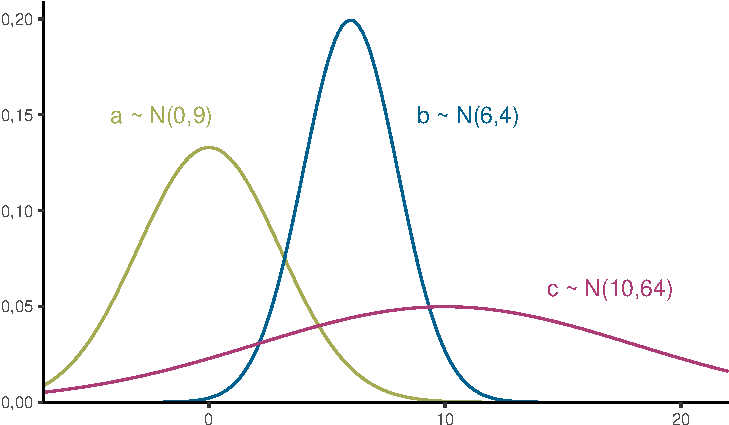
\includegraphics[width=.6\linewidth]{Skript_Statistik_2021_files/figure-latex/norms-1} 

}

\caption{Dichtefunktionen verschiedener Normalverteilungen}\label{fig:norms}
\end{figure}

Die Normalverteilung (auch: Gaußverteilung, engl. \emph{normal distribution}) ist unimodal und symmetrisch. Die Normalverteilung ist eine theoretische Verteilung, für die bekannt ist, mit welcher Wahrscheinlichkeit bestimmte Werte unter- und überschritten werden bzw. mit welcher Wahrscheinlichkeit Werte in einem bestimmten Intervall liegen.

Die Dichtefunktion einer Normalverteilung hat eine markante Glockenform (s. Abbildungen~\ref{fig:norms} und \ref{fig:stdnorm}). Die beiden Wendepunkte einer Normalverteilung (also dort, wo die Steigung zwischen zu- und abnehmend wechselt; oder mathematisch: wo die Ableitung der Dichtefunktion einen Extremwert annimmt) sind je eine Standardabweichung vom Mittelwert entfernt.

Die Dichtefunktion nimmt nie den Wert Null an -- Extremwerte sind also sehr selten bzw. unwahrscheinlich, aber nie unmöglich. Perfekte Normalverteilungen kommen in empirischen Beobachtungen nicht vor, sondern nur Annäherungen.

Da es sich um eine \emph{theoretische} Verteilung handelt, ist die Normalverteilung zunächst insbesondere in Bezug auf die Grundgesamtheit interessant. Im Kontext der Grundgesamtheit wird das arithmetische Mittel mit \(\mu\) (\enquote{Mü}) und die Standardabweichung mit \(\sigma\) (\enquote{Sigma}) bezeichnet (s. Tabelle~\ref{tab:param}).

\begin{table}

\caption{\label{tab:param}Bezeichnung von Parametern in Stichprobe und Grundgesamtheit}
\centering
\begin{tabular}[t]{lll}
\toprule
Parameter & Stichprobe & Grundgesamtheit\\
\midrule
Anzahl Elemente & $n$ & $N$\\
Arithmetisches Mittel & $\bar{x}$ & $\mu$\\
Varianz & $s^2$ & $\sigma^2$\\
Standardabweichung & $s$ & $\sigma$\\
\bottomrule
\end{tabular}
\end{table}

Jede Normalverteilung lässt sich anhand von zwei Parametern beschreiben: ihr arithmetisches Mittel und ihre Standardabweichung. Normalverteilte Grundgesamtheiten werden so notiert:

\nopagebreak

\[\begin{aligned}
x \sim N(\mu,\enspace\sigma^2)
\end{aligned}
\label{eq:norm}\]

Der Mittelwert \(\mu\) bestimmt die Lage der Kurve auf der x-Achse, die Varianz \(\sigma^2\) bestimmt die \enquote{Stauchung} der Kurve (je größer desto flacher). Es gibt also unendlich viele verschiedene Normalverteilungen (s. Abbildung~\ref{fig:norms}).

\hypertarget{standardnormalverteilung}{%
\section{Standardnormalverteilung}\label{standardnormalverteilung}}

Die Standardnormalverteilung (engl. \emph{standard normal distribution}) ist sozusagen das Grundmuster aller Normalverteilungen. Sie hat den Mittelwert \(\mu=0\) und die Standardabweichung \(\sigma=1\) (s. Abbildung~\ref{fig:stdnorm}).

Alle Normalverteilungen lassen sich durch die \(z\)-Transformation auf die Standardnormalverteilung standardisieren.

\begin{figure}[!h]

{\centering 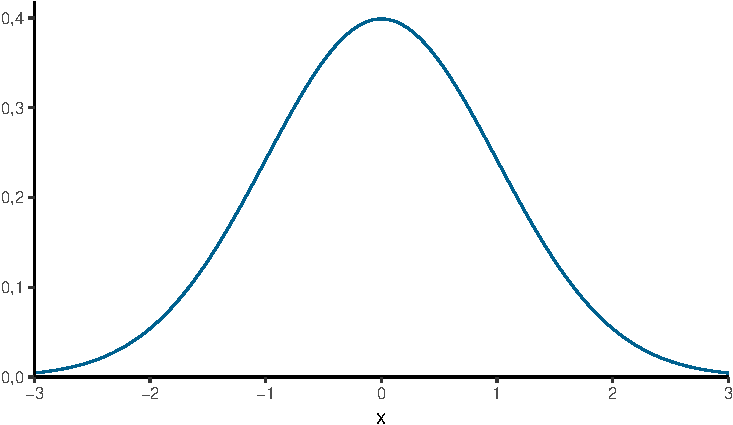
\includegraphics[width=.6\linewidth]{Skript_Statistik_2021_files/figure-latex/stdnorm-1} 

}

\caption{Dichtefunktion der Standardnormalverteilung}\label{fig:stdnorm}
\end{figure}

\hypertarget{crash-kurs-wahrscheinlichkeitsrechnung}{%
\section{Crash-Kurs Wahrscheinlichkeitsrechnung}\label{crash-kurs-wahrscheinlichkeitsrechnung}}

Ein Zufallsexperiment ist ein beliebig oft wiederholbarer, nach bestimmten Vorschriften ausgeführter Versuch, dessen Ergebnis zufallsbedingt ist (d.~h. nicht eindeutig voraussagbar ist).

Jedem zufälligen Ereignis \(A\) ist eine bestimmte \enquote{Wahrscheinlichkeit des Auftretens} (engl. \emph{probability}) \(P(A)\) zugeordnet, die der Ungleichung \(0 \leq P(A) \leq 1\) genügt (d.~h. zwischen 0 und 1 liegt).

Die Wahrscheinlichkeit eines sicheren Ergebnisses A ist \(P(A) = 1\). Hingegen würde \(P(B) = 0\) bedeuten, dass das Ereignis B nicht eintreten kann. Die Summe der Wahrscheinlichkeiten aller möglichen Ereignisse beträgt 1.

Der \emph{Additionssatz} besagt: Die Wahrscheinlichkeit, dass eins von verschiedenen zufälligen, sich gegenseitig ausschließenden Ereignissen eintritt, ist die Summe ihrer Wahrscheinlichkeiten.

Der \emph{Multiplikationssatz} besagt: Die Wahrscheinlichkeit für das Eintreten zweier voneinander unabhängiger Ereignisse ist gleich dem Produkt der Einzelwahrscheinlichkeiten.

\hypertarget{wahrscheinlichkeitsdichtefunktionen}\) sowie die Angelpunkte \(Q_1=x_{25\%}\) und \(Q_3=x_{75\%}\) kennengelernt.

Die Fläche unter einer Wahrscheinlichkeitsdichtefunktion innerhalb der Limits \(-\infty\) und \(x_p\) beträgt \(p\). Für einen zufälligen Wert \(x\) ist die Wahrscheinlichkeit \(P(x < x_p) = p\), dass er kleiner als \(x_p\) ausfällt.
Für die Standardnormalverteilung finden sich die \(p\)-Werte für positive \(z\) in der \href{Formelsammlung\%20und\%20Wertetabellen.pdf}{Formelsammlung}.\footnote{Manchmal wird die Funktion \(z_p \rightarrow P(z < z_p)\) für normalverteilte Werte auch mit \(\Phi(z)\) bezeichnet (z.~B. in \protect\hyperlink{ref-bahrenberg}{Bahrenberg, Giese und Nipper 2010}).}

\hypertarget{wahrscheinlichkeitsrechnung-mit-standardnormalverteilung}{%
\section{Wahrscheinlichkeitsrechnung mit Standardnormalverteilung}\label{wahrscheinlichkeitsrechnung-mit-standardnormalverteilung}}

Für die im Rest dieser Sitzung vorgestellten Verfahren müssen folgende Voraussetzungen gegeben sein:

\begin{itemize}
\tightlist
\item
  Die Grundgesamtheit ist (annähernd) normalverteilt.
\item
  Arithmetisches Mittel \(\mu\) und Standardabweichung \(\sigma\) der Grundgesamtheit sind bekannt.
\end{itemize}

Die Verfahren sollen anhand eines Beispiels illustriert werden: Es sei bekannt, dass der Luftdruck auf dem Feldberg annähernd normalverteilt ist, und zwar mit dem arithmetischen Mittel \(\mu=1003\) und Varianz \(\sigma^2=73\). Graphisch stellt sich die Wahrscheinlichkeitsdichtefunktion wie in Abbildung~\ref{fig:dens} dar.

\begin{figure}[t]

{\centering 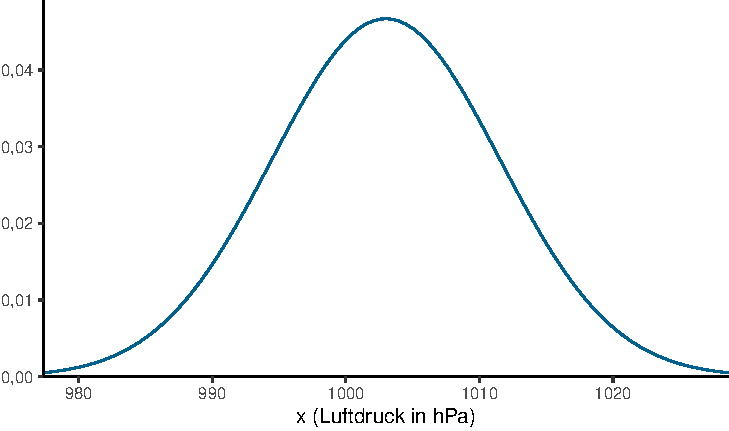
\includegraphics[width=.6\linewidth]{Skript_Statistik_2021_files/figure-latex/dens-1} 

}

\caption{Theoretische Wahrscheinlichkeitsdichtefunktion des Luftdrucks}\label{fig:dens}
\end{figure}

Wir können auch (analog zu Formel~\eqref{eq:norm}) schreiben:

\[
x \sim N(1003,\enspace73)
\]

Daraus ergibt sich für die Standardabweichung \(\sigma\):
\nopagebreak

\[\begin{aligned}
\sigma&=\sqrt{\sigma^2}\\
&=\sqrt{73}\\
&\approx8{,}54
\end{aligned}\]

\hypertarget{unter}{%
\subsection{Unterschreitungswahrscheinlichkeit}\label{unter}}

Die einfachste Art der Fragestellung ist nun, mit welcher Wahrscheinlichkeit ein bestimmter Wert \(x_p\) unterschritten wird.

Nehmen wir an, es sei gefragt, mit welcher Wahrscheinlichkeit zu einem beliebigen Zeitpunkt der Luftdruck weniger als 1015~hPa beträgt. Anders gesagt interessiert uns der Anteil der Fläche unter der Verteilung, der zwischen \(-\infty\) und \(x_p=1015\) liegt (s. Abbildung~\ref{fig:unter}).

\begin{figure}[H]

{\centering 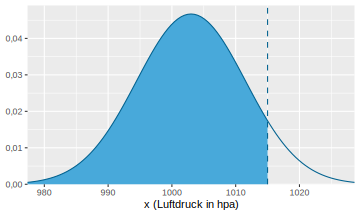
\includegraphics[width=.6\linewidth]{Skript_Statistik_2021_files/figure-latex/unter-1} 

}

\caption{Unterschreitung eines Messwerts}\label{fig:unter}
\end{figure}

Um den entsprechenden Wert für \(P(x < x_p)\) (also die Wahrscheinlichkeit, dass ein zufälliges \(x\) unser Perzentil \(x_p\) unterschreitet) in Erfahrung zu bringen, müssen wir die Verteilung zunächst standardisieren. Der Wert \(z_p\) ergibt sich aus der Formel für die \(z\)-Transformation, diesmal jedoch mit \(\mu\) statt \(\bar{x}\) und \(\sigma\) statt \(s\), da es sich um die Grundgesamtheit handelt:

\[\begin{aligned}
    z_p &= \frac{x_p-\mu}{\sigma} \\[4pt]
        &\approx \frac{1015-1003}{8{,}54}\\[4pt]
        &\approx 1{,}41
  \end{aligned}
\]

Graphisch ist das standardisierte Perzentil in Abbildung~\ref{fig:z} dargestellt.

\begin{figure}[H]

{\centering 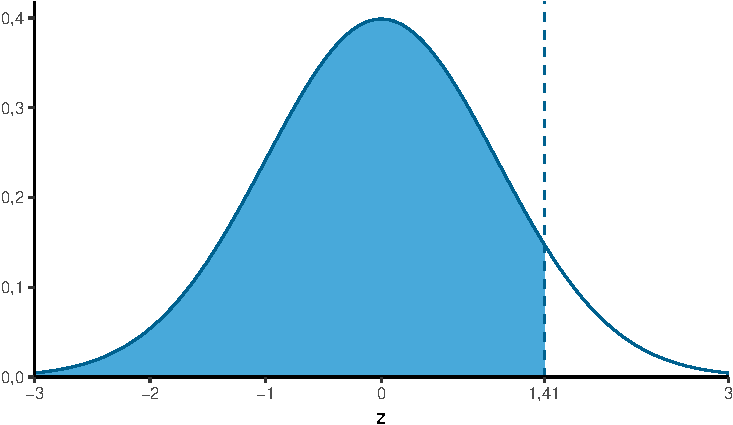
\includegraphics[width=.6\linewidth]{Skript_Statistik_2021_files/figure-latex/z-1} 

}

\caption{Standardnormalverteilung des Luftdrucks}\label{fig:z}
\end{figure}

Die \protect\hyperlink{formeln}{Formelsammlung} gibt für \(z\)-Werte die Wahrscheinlichkeit ihrer Unterschreitung in ener Normalverteilung an. Diese Wahrscheinlichkeit kann notiert werden als \(P(z<z_p)\).

Der \protect\hyperlink{formeln}{Formelsammlung} können wir den Wert \(P(z < 1,41) \approx 0,9207\) entnehmen. Die Wahrscheinlichkeit, dass der Luftdruck zu einem zufälligen Zeitpunkt weniger als 1015 hPA beträgt, ist somit 92,07\%.

\begin{rtip}
In R lässt sich die Unterschreitungswahrscheinlichkeit eines $z$-Werts mit dem Befehl \verb|pnorm()| ermitteln.
\end{rtip}

\hypertarget{uxfcberschreitungswahrscheinlichkeit}{%
\subsubsection{Überschreitungswahrscheinlichkeit}\label{uxfcberschreitungswahrscheinlichkeit}}

Wird nach der Wahrscheinlichkeit der Überschreitung eines Werts gefragt, ist in anderen Worten die Fläche unter der Wahrscheinlichkeitsdichtefunktion zwischen \(x_p\) und \(\infty\) gemeint. Wir bleiben bei unserem Beispiel \(x_p=1015\) (s. Abbildung~\ref{fig:ueber}).

\begin{figure}[!h]

{\centering 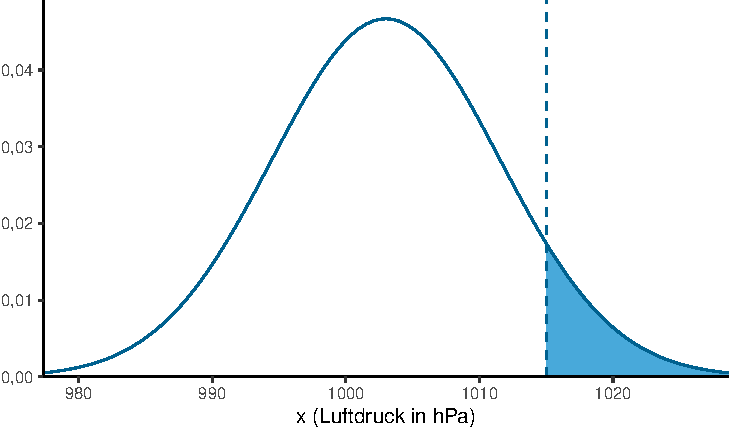
\includegraphics[width=.6\linewidth]{Skript_Statistik_2021_files/figure-latex/ueber-1} 

}

\caption{Überschreitung eines Messwerts}\label{fig:ueber}
\end{figure}

Hier können wir genauso wie bei der Unterschreitung \(z_p=1{,}41\) errechnen.

Jetzt stehen wir zunächst vor dem Problem, dass die \(p\)-Werte in der Tabelle immer die Wahrscheinlichkeit der Unterschreitung darstellen. Wir wissen jedoch: Die gesamte Fläche unter der Verteilung ist 1, und die Wahrscheinlichkeiten der Unter- und Überschreitung sind komplementär, d.~H. einer von beiden Fällen tritt sicher (mit einer Wahrscheinlichkeit von 100\%) ein. (Den Sonderfall \(x=x_p\) können wir bei stetigen Variablen vernachlässigen.)

Hieraus ergibt sich ganz allgemein:

\[
  \begin{aligned}
    P(x \geq x_p) = 1-P(x<x_p)
  \end{aligned}
  \label{eq:ueber}
\]

Und für unser Beispiel:

\[
  \begin{aligned}
    P(x \geq 1015) &= 1-P(x < 1015) \\
    &\approx1-P(z < 1,41)\\
    &\approx1-0{,}9207\\
    &= 0{,}0793
  \end{aligned}
\]

In 7,93\% der Fälle beträgt der Luftdruck also über 1015~hPA.

\hypertarget{negativer-z-wert}{%
\subsubsection{\texorpdfstring{Negativer \(z\)-Wert}{Negativer z-Wert}}\label{negativer-z-wert}}

Wenn nach der Unterschreitungswahrscheinlichkeit eines unterdurchschnittlichen Werts gefragt ist (z.~B. 990~hPA), dann ergibt sich ein negativer Wert für \(z_p\):

\begin{equation}
  \begin{aligned}
    z_p &= \frac{x_p-\mu}{\sigma} \\[4pt]
        &= \frac{990-1003}{8{,}54} \\[4pt]
        &\approx -1{,}52
  \end{aligned}
\end{equation}

Die \href{Formelsammlung\%20und\%20Wertetabellen.pdf}{Formelsammlung} enthält keine \(p\) für negative \(z_p\). Da die Standardnormalverteilung jedoch um \(z=0\) symmetrisch ist, gilt ganz allgemein:

\[
  \begin{aligned}
    P(z < -z_p) = 1 - P(z < z_p)
  \end{aligned}
  \label{eq:neg}
\]

Für unser Beispiel ergibt sich (mit dem Wert \(P(z < 1,52) = 0{,}9357\) aus der Tabelle):

\[
  \begin{aligned}
    P(z < -1,52) &= 1 - P(z < 1,52) \\
    &\approx 1-0{,}9357 \\
    &=0{,}0643
  \end{aligned}
\]

Ein Luftdruck von 990~hPa wird also nur in ca. 6,43\% der Fälle unterschritten.

\begin{rtip}
Der Befehl \verb|pnorm()| funktioniert auch mit negativen $z$-Werten.
\end{rtip}

\hypertarget{wert-in-einem-intervall}{%
\subsubsection{Wert in einem Intervall}\label{wert-in-einem-intervall}}

Nun wollen wir wissen, mit welcher Wahrscheinlichkeit ein zufälliger Meßwert zwischen 1005 und 1015~hPa liegt. Graphisch ist dies in Abbildung~\ref{fig:intervall} aufbereitet.

\begin{figure}[!h]

{\centering 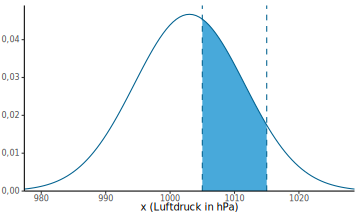
\includegraphics[width=.6\linewidth]{Skript_Statistik_2021_files/figure-latex/intervall-1} 

}

\caption{Messwertintervall}\label{fig:intervall}
\end{figure}

Rechnerisch müssen wir also von den (günstigen) Fällen, in denen 1015 hPA unterschritten werden, noch jene (ungünstige) Fälle abziehen, in denen die 1005 hPA \emph{ebenfalls} unterschritten werden.

Ganz allgemein heißt das für die Untergrenze \(x_u\) und die Obergrenze \(x_o\):

\[\begin{aligned}
    P(x_{u} \leq x < x_{o}) = P(x < x_{o}) - P(x < x_{u})
  \end{aligned}
  \label{eq:intervall}
\]

Für unseren Fall ist \(x_u=1005\) und \(x_o=1015\). In den \protect\hyperlink{unter}{vorherigen Aufgaben} haben wir \(z_o\approx1,41\) bereits ermittelt. Wir müssen aber noch \(z_u\) ermitteln:

\[\begin{aligned}
    z_u &= \frac{x_u-\mu}{\sigma} \\[4pt]
        &= \frac{1005-1003}{8{,}54}  \\[4pt]
        &\approx 0{,}23
\end{aligned}\]

Dann können wir die entsprechende Wahrscheinlichkeit berechnen, indem wir wieder die Werte aus der \href{Formelsammlung\%20und\%20Wertetabellen.pdf}{Formelsammlung} einsetzen:

\[
  \begin{aligned}
    P(1005 \leq x < 1015) &= P(x < 1015) - P(x < 1005) \\
    &\approx P(z < 1{,}41) - P(z < 0{,}23) \\
    &\approx 0{,}9207- 0{,}5910  \\
    &= 0{,}3297
  \end{aligned}
\]

Der Luftdruck liegt also mit einer Wahrscheinlichkeit von 32,97\% zwischen 1005 und 1015~hPa.

\hypertarget{gesuchter-wert-bei-gegebener-wahrscheinlichkeit}{%
\subsubsection{Gesuchter Wert bei gegebener Wahrscheinlichkeit}\label{gesuchter-wert-bei-gegebener-wahrscheinlichkeit}}

Die Fragerichtung lässt sich umdrehen: Welche Marke wird beim Messen des Luftdrucks nur in 5\% der Fälle überschritten?

5\% Überschreitungswahrscheinlichkeit entsprechen einer Unterschreitungswahrscheinlichkeit von 95\%. Welcher Wert wird also mit 95\% Wahrscheinlichkeit unterschritten?

Der Tabelle entnehmen wir, dass einer Unterschreitungswahrscheinlichkeit von 0,95 ein \(z\)-Wert zwischen 1,64 und 1,65 entspricht. Da es bei dieser Fragestellungen oft darum geht, einen \enquote{kritischen} Wert zu nennen, der nur in Ausnahmefällen überschritten wird, nehmen wir hier üblicherweise den extremeren Wert, also \(z_{95\%}\approx 1,65\).

Mit der umgekehrten \(z\)-Transformation erhalten wir:

\[
  \begin{aligned}
    x_{95\%}&=z_{95\%}\cdot \sigma + \mu \\
       &\approx 1{,}65\cdot 8{,}54 + 1003\\
       &\approx 1017{,}10
  \end{aligned}
\]

Die Marke von 1017,10~hPa wird also nur in 5\% der Fälle überschritten.

\begin{rtip}
Das Perzentil für eine gegebene Unterschreitungswahrscheinlichkeit lässt sich in R mit \verb|qnorm()| bestimmen.
\end{rtip}

\hypertarget{gesuchte-grenzwerte-eines-intervalls}{%
\subsubsection{Gesuchte Grenzwerte eines Intervalls}\label{gesuchte-grenzwerte-eines-intervalls}}

Eine übliche Art der Fragestellung ist auch: Zwischen welchen beiden Werten liegen die mittleren 85\% der Fälle (s. Abbiddung~\ref{fig:mitte})?

\begin{figure}[!h]

{\centering 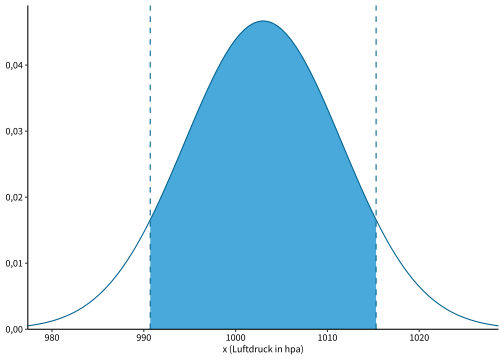
\includegraphics[width=.6\linewidth]{Skript_Statistik_2021_files/figure-latex/mitte-1} 

}

\caption{Die mittleren 85\% der Normalverteilung}\label{fig:mitte}
\end{figure}

Da die Verteilung symmetrisch ist, teilen sich die ungünstigen 15\% der Fälle gleichmäßig an den oberen und unteren Rand der Verteilung auf. Die Obergrenze \(x_o\) ist also der Wert, der zu 7,5\% über- und damit zu 92,5\% unterschritten wird.

Der Tabelle entnehmen wir den Wert \(z_o=z_{92,5\%}\approx1{,}44\).

Die Untergrenze ist entsprechend der Wert, der in 7,5\% der Fälle unterschritten wird.

Der Wert für \(z_u=z_{7{,}5\%}\) ist in der Tabelle nicht enthalten. Weil die Verteilung aber symmetrisch ist, wissen wir uns zu helfen:

\[
  \begin{aligned}
    z_u=z_{7{,}5\%}=-z_{92{,}5\%}\approx-1{,}44
  \end{aligned}
  \]

Die absoluten Werte ergeben sich schließlich aus:

\[
  \begin{aligned}
    x_u&=z_u\cdot \sigma + \mu \\
    &\approx-1{,}44 \cdot 8{,}54 + 1003\\
    &\approx990{,}70
  \end{aligned}
\]

Und:

\[
  \begin{aligned}
    x_o&=z_o\cdot \sigma + \mu  \\
    &\approx1{,}44 \cdot 8{,}54 + 1003\\
    & \approx 1015{,}30
  \end{aligned}
\]

Die mittleren 85\% der Messwerte liegen also zwischen 990,7 und 1015,3~hPa.

\hypertarget{tipps-zur-vertiefung-2}{%
\section*{Tipps zur Vertiefung}\label{tipps-zur-vertiefung-2}}
\addcontentsline{toc}{section}{Tipps zur Vertiefung}

\hypertarget{variationskoeffizient-1}{%
\subsection{Variationskoeffizient}\label{variationskoeffizient-1}}

\begin{itemize}
\tightlist
\item
  Kapitel 3.3.4 in \protect\hyperlink{ref-delange}{Lange und Nipper} (\protect\hyperlink{ref-delange}{2018})
\item
  Kapitel 4.2.2 in \protect\hyperlink{ref-bahrenberg}{Bahrenberg, Giese und Nipper} (\protect\hyperlink{ref-bahrenberg}{2010})
\item
  YouTube-Kanal \enquote{Kurzes Tutorium Statistik}: \href{https://www.youtube.com/watch?v=3oZrS3ZWVcA}{Streumaße - Varianz, Standardabweichung, Variationskoeffizient und mehr!}
\item
  \emph{Englisch:} Kapitel 2.3 in \protect\hyperlink{ref-burt}{Burt und Barber} (\protect\hyperlink{ref-burt}{1996})
\end{itemize}

\hypertarget{z-transformation-1}{%
\subsection{\texorpdfstring{\(z\)-Transformation}{z-Transformation}}\label{z-transformation-1}}

\begin{itemize}
\tightlist
\item
  Kapitel~2.4 in \protect\hyperlink{ref-bortz}{Bortz und Schuster} (\protect\hyperlink{ref-bortz}{2010})
\item
  Kapitel~3.5.2 in \protect\hyperlink{ref-delange}{Lange und Nipper} (\protect\hyperlink{ref-delange}{2018})
\item
  Kapitel~4.2.2 in \protect\hyperlink{ref-bahrenberg}{Bahrenberg, Giese und Nipper} (\protect\hyperlink{ref-bahrenberg}{2010})
\item
  Kapitel~3.3.3 in \protect\hyperlink{ref-benninghaus}{Benninghaus} (\protect\hyperlink{ref-benninghaus}{2007})
\item
  YouTube-Kanal \enquote{Methodenlehre Mainz}: \href{https://www.youtube.com/watch?v=AiucvUlIP8k}{WT.012.09 Äpfel mit Birnen vergleichen: Die z-Standardisierung}
\item
  \emph{Englisch:} Kapitel 6.3 in \protect\hyperlink{ref-burt}{Burt und Barber} (\protect\hyperlink{ref-burt}{1996})
\end{itemize}

\hypertarget{normalverteilung-1}{%
\subsection{Normalverteilung}\label{normalverteilung-1}}

\begin{itemize}
\tightlist
\item
  Kapitel 5.4 in \protect\hyperlink{ref-bortz}{Bortz und Schuster} (\protect\hyperlink{ref-bortz}{2010})
\item
  Kapitel 7.3.2.2 und 7.3.2.3 in \protect\hyperlink{ref-delange}{Lange und Nipper} (\protect\hyperlink{ref-delange}{2018})
\item
  Kapitel 5.2.2 in \protect\hyperlink{ref-bahrenberg}{Bahrenberg, Giese und Nipper} (\protect\hyperlink{ref-bahrenberg}{2010})
\item
  YouTube-Kanal \enquote{Mathe by Daniel Jung}: \href{https://www.youtube.com/watch?v=_f1vgWUiavY}{Was ist die Normalverteilung, Gauß-Verteilung, Schaubilder, Übersicht}
\item
  \emph{Englisch:} Kapitel 6.3 in \protect\hyperlink{ref-burt}{Burt und Barber} (\protect\hyperlink{ref-burt}{1996})
\end{itemize}

\hypertarget{wahrscheinlichkeitsdichtefunktion}{%
\subsection{Wahrscheinlichkeitsdichtefunktion}\label{wahrscheinlichkeitsdichtefunktion}}

\begin{itemize}
\tightlist
\item
  Kapitel 5.3 in \protect\hyperlink{ref-bortz}{Bortz und Schuster} (\protect\hyperlink{ref-bortz}{2010})
\item
  Kapitel 7.3.2.1 in \protect\hyperlink{ref-delange}{Lange und Nipper} (\protect\hyperlink{ref-delange}{2018})
\item
  Kapitel 5.2.2 in \protect\hyperlink{ref-bahrenberg}{Bahrenberg, Giese und Nipper} (\protect\hyperlink{ref-bahrenberg}{2010})
\item
  YouTube-Kanal \enquote{Kurzes Tutorium Statistik}: \href{https://www.youtube.com/watch?v=DoHTsDrzAQk}{Zufallsvariable, Massenfunktion, Dichtefunktion und Verteilungsfunktion}
\item
  \emph{Englisch:} Kapitel 6.1 in \protect\hyperlink{ref-burt}{Burt und Barber} (\protect\hyperlink{ref-burt}{1996})
\end{itemize}

\hypertarget{uxfcbungsaufgaben-2}{%
\section*{Übungsaufgaben}\label{uxfcbungsaufgaben-2}}
\addcontentsline{toc}{section}{Übungsaufgaben}

\hypertarget{aufgabe-3-1}{%
\subsection{Aufgabe~3-1}\label{aufgabe-3-1}}

\protect\hyperlink{loesung-3-1}{zur~Lösung}

\begin{enumerate}
\def\labelenumi{\alph{enumi})}
\item
  Führen Sie eine \(z\)-Transformation der folgenden Verteilung durch:

\begin{verbatim}
-16,93  -16,09  -10,97  -3,77  -25,55  -20,57  -23,61  -25,9  -27,08
\end{verbatim}
\item
  Sie kennen das arithmetische Mittel (221,54) und die Varianz (13,02) einer Verteilung. Welche \(x\)-Werte entsprechen diesen \(z\)-Werten?

\begin{verbatim}
0,9  -1,4  1,12  -0,33  2,22  0,15  2,87  0,4  -1,54  0,13  -0,17  0,68
\end{verbatim}
\end{enumerate}

\hypertarget{aufgabe-3-2}{%
\subsection{Aufgabe~3-2}\label{aufgabe-3-2}}

\protect\hyperlink{loesung-3-2}{zur~Lösung}

Gegeben sei eine Normalverteilung beschrieben durch:

\[x \sim N(32{,}2,\enspace19{,}36)\]

\begin{enumerate}
\def\labelenumi{\alph{enumi})}
\item
  Mit welcher Wahrscheinlichkeit werden die folgenden Werte unterschritten?

\begin{verbatim}
40,63  20,77  33,41  44,95  41,91  32,95
\end{verbatim}
\item
  Welche Werte werden jeweils mit der folgenden Wahrscheinlichkeit über(!)schritten?

\begin{verbatim}
1,5%  2,5%  5%  13%  50%  90%  99%  99,5%
\end{verbatim}
\item
  In welchem Bereich liegen die mittleren 95\% der Werte?
\item
  Wie wahrscheinlich ist es, dass ein Wert zwischen 30 und 40 liegt?
\end{enumerate}

\hypertarget{aufgabe-3-3}{%
\subsection{Aufgabe~3-3}\label{aufgabe-3-3}}

\protect\hyperlink{loesung-3-3}{zur~Lösung}

Deiche werden durch Wasserdruck bei Hochwasser belastet und dadurch beschädigt. Bei einem 12~m hohen Deich gilt als kritische Marke ein Wasserstand von 10~m. Die jährlichen Höchstwasserstände des Flusses sind normalverteilt mit einem Mittelwert von 9,01~m und einer Standardabweichung von 2,23~m.

In den folgenden Teilaufgaben beantworten wir Schritt für Schritt die Frage, wie wahrscheinlich es (für ein beliebiges Jahr) ist, dass der Deich das jährliche Hochwasser ohne Beschädigung übersteht, d.~h. dass ein Höchstwasserstand von 10~m oder weniger eintritt.

\begin{enumerate}
\def\labelenumi{\alph{enumi})}
\tightlist
\item
  Zeichnen Sie die Wahrscheinlichkeitsdichtefunktion (ganz grob, ohne \(y\)-Achse).
\item
  Markieren Sie den kritischen Wert 10~m.
\item
  Welchem \(z\)-Wert entspricht die kritische Marke von 10~?
\item
  Mit welcher Wahrscheinlichkeit bleibt der Deich in einem gegebenen Jahr unbeschädigt (Höchstwasserstand unter der kritischen Marke von 10~m)?
\end{enumerate}

\hypertarget{aufgabe-3-4}{%
\subsection{Aufgabe~3-4}\label{aufgabe-3-4}}

\protect\hyperlink{loesung-3-4}{zur~Lösung}

Wir bleiben beim Deich aus Aufgabe 3.

\begin{enumerate}
\def\labelenumi{\alph{enumi})}
\tightlist
\item
  Mit welcher Wahrscheinlichkeit wird der Deich beschädigt (Wasserstand über 10~m)?
\item
  Mit welcher Wahrscheinlichkeit wird der Deich nicht nur beschädigt, sondern läuft über (Wasserstand über 12~m)?
\item
  Mit welcher Wahrscheinlichkeit wird der Deich beschädigt, läuft aber nicht über (Wasserstand zwischen 10 und 12~m)?
\item
  In welchen Grenzen liegen die mittleren 80\% der Hochwasserstände?
\end{enumerate}

\hypertarget{aufgabe-3-5}{%
\subsection{Aufgabe~3-5}\label{aufgabe-3-5}}

\protect\hyperlink{loesung-3-5}{zur~Lösung}

Es ist ein neuer Deich zu bauen, der so sicher sein soll, dass er nur alle 200 Jahre vom Hochwasser übertreten wird.

\begin{enumerate}
\def\labelenumi{\alph{enumi})}
\tightlist
\item
  Welcher Wahrscheinlichkeitswert \(p=P(x < x_p)\) ist anzuwenden, d.~h. wie wahrscheinlich ist die \emph{Unterschreitung} eines \enquote{zweihundertjährigen Hochwassers}?
\item
  Mit welchem \(z\)-Wert korrespondiert der gesuchte Wert \(x_p\)?
\item
  Wie hoch muss dieser Deich sein? (Welcher Wert \(x_p\) entspricht diesem \(z_p\)?)
\end{enumerate}

\hypertarget{aufgabe-3-6}{%
\subsection{Aufgabe~3-6}\label{aufgabe-3-6}}

\protect\hyperlink{loesung-3-6}{zur~Lösung}

Die jährlichen Niederschlagsmengen in Mittelstedt betragen im Durchschnitt 400~mm bei annähernder Normalverteilung und einer Standardabweichung von 100~mm.

\begin{enumerate}
\def\labelenumi{\alph{enumi})}
\tightlist
\item
  Wie groß ist die Wahrscheinlichkeit, dass mehr als 500~mm Niederschlag fallen?
\item
  Wie oft pro hundert Jahre kann mit weniger als 200~mm Niederschlag gerechnet werden?
\item
  Mit welcher Wahrscheinlichkeit fallen zwischen 200 und 550~mm Niederschlag?
\item
  Welche Niederschlagsmenge wird wahrscheinlich in nur 2 von 100 Jahren übertroffen?
\item
  In welchen Grenzen liegen die mittleren 75\% der jährlichen Niederschlagsmenge?
\end{enumerate}

\hypertarget{aufgabe-3-7}{%
\subsection{Aufgabe~3-7}\label{aufgabe-3-7}}

\protect\hyperlink{loesung-3-7}{zur~Lösung}

Errechnen Sie für die Verteilungen in \protect\hyperlink{aufgabe-2-5}{Aufgabe 5 aus Sitzung 2} jeweils den Variationskoeffizienten.

\hypertarget{schuxe4tzstatistik}{%
\chapter{Schätzstatistik}\label{schuxe4tzstatistik}}

\hypertarget{lernziele-dieser-sitzung-3}{%
\subsection*{Lernziele dieser Sitzung}\label{lernziele-dieser-sitzung-3}}
\addcontentsline{toc}{subsection}{Lernziele dieser Sitzung}

Sie können\ldots{}

\begin{itemize}
\tightlist
\item
  eine Punktschätzung für \(\mu\) und \(\sigma\) durchführen.
\item
  den Standardfehler der Stichprobenverteilung von \(\bar{x}\) bestimmen.
\item
  eine Intervallschätzung für \(\mu\) durchführen.
\end{itemize}

\hypertarget{lehrvideos-sommersester-2020}{%
\subsection*{Lehrvideos (Sommersester 2020)}\label{lehrvideos-sommersester-2020}}
\addcontentsline{toc}{subsection}{Lehrvideos (Sommersester 2020)}

\begin{itemize}
\tightlist
\item
  \href{https://video01.uni-frankfurt.de/Mediasite/Play/7f5b3002871a4b18859db90d937e5f8a1d}{4a) Alphafehler}

  \begin{itemize}
  \tightlist
  \item
    In diesem Video gibt es einen Fehler: In Schritt c) der Übungsaufgabe setze ich den falschen Wert für \(\mu\) ein. Die Werte müssten stattdessen \(x_{(1-\alpha/2)}=27{,}84\) und \(x_{\alpha/2}=20{,}16\) betragen.
  \end{itemize}
\item
  \href{https://video01.uni-frankfurt.de/Mediasite/Play/393be1f574c643f9a045a6b4cc60a4511d}{4b) Stichprobenverteilung}
\item
  \href{https://video01.uni-frankfurt.de/Mediasite/Play/ace60129a0c94894a66349f56e0b24a31d}{4c) Schätzungen}
\end{itemize}

\hypertarget{stichprobenverteilung}{%
\section{Stichprobenverteilung}\label{stichprobenverteilung}}

\begin{quote}
Die Stichprobenverteilung ist eine theoretische Verteilung, welche die möglichen Ausprägungen eines statistischen Kennwertes (z.~B. \(\bar{x}\)) sowie deren Auftretenswahrscheinlichkeit beim Ziehen von Zufallsstichproben des Umfanges \(n\) beschreibt. (\protect\hyperlink{ref-bortz}{Bortz und Schuster 2010}: 83)
\end{quote}

Hier ist zunächst die theoretische Verteilung des Mittelwerts einer Stichprobe relevant. Insbesondere interessiert uns, wie sich die theoretische Verteilung des Mittelwerts abhängig von der Stichprobengröße verhält.

\hypertarget{szenario-1-normalverteilte-grundgesamtheit}{%
\subsection{Szenario 1: Normalverteilte Grundgesamtheit}\label{szenario-1-normalverteilte-grundgesamtheit}}

Die Grundgesamtheit (Population) einer Variable \(x\) sei normalverteilt mit \(\mu=50\) und \(\sigma^2=25\). Wir können also schreiben:

\nopagebreak

\[ x \sim N(50, \enspace 25) \]

Die Standardabweichung der Population beträgt entsprechend:

\nopagebreak

\[\begin{aligned}
\sigma&=\sqrt{\sigma^2}\\[4pt]
&=\sqrt{25}=5\end{aligned}\]

Graphisch ist die Dichtefunktion der Verteilung in Abbildung~\ref{fig:pop} veranschaulicht.

\begin{figure}[!h]

{\centering 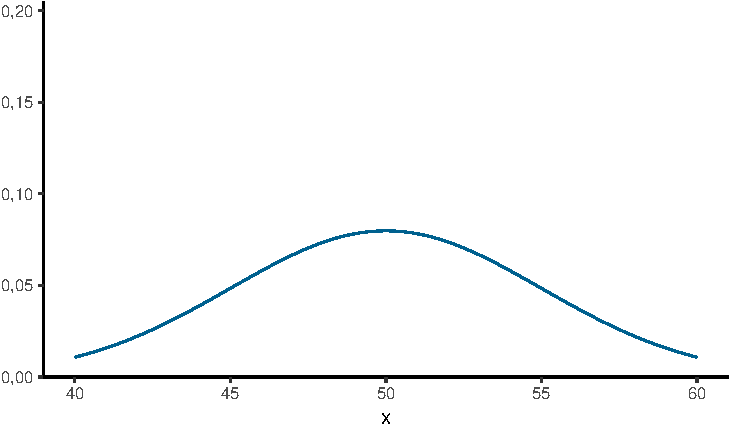
\includegraphics[width=.6\linewidth]{Skript_Statistik_2021_files/figure-latex/pop-1} 

}

\caption{Dichtefunktion der Grundgesamtheit}\label{fig:pop}
\end{figure}

Wenn eine einzelne Stichprobe der Größe \(n=3\) aus dieser Verteilung gezogen würde, hätte sie drei konkrete Werte (\(x_1\), \(x_2\) und \(x_3\)) sowie ein konkretes arithmetisches Mittel (\(\bar{x}\)).

Es lässt sich jedoch auch eine Wahrscheinlichkeitsdichtefunktion der Mittelwerte \emph{aller theoretisch möglichen Stichproben} der Größe \(n=3\) (und zusätzlich der Größe \(n=6\)) zeichnen (s. Abbildung~\ref{fig:stich}).

\begin{figure}[!h]

{\centering 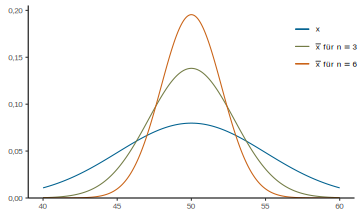
\includegraphics[width=.6\linewidth]{Skript_Statistik_2021_files/figure-latex/stich-1} 

}

\caption{Dichtefunktionen der Stichprobenverteilungen}\label{fig:stich}
\end{figure}

\hypertarget{erwartungswert}{%
\subsubsection{Erwartungswert}\label{erwartungswert}}

Es fällt auf, dass die Stichprobenverteilungen für \(\bar{x}\) normalverteilt sind und um das arithmetische Mittel der Grundgesamtheit (\(\mu\)) symmetrisch sind.

Das arithmetische Mittel der Stichprobenverteilung \(\mu_{\bar{x}}\) wird auch als \textbf{Erwartungswert} (engl. \emph{expected value}) von \(\bar{x}\) bezeichnet. Es gilt:

\nopagebreak

\[
\mu_{\bar{x}} = \mu
\label{eq:mean}
\]

Wir können auch sagen: \(\bar{x}\) ist ein \enquote{erwartungstreuer} Schätzparameter für \(\mu\); nicht weil er in der Empirie zwangsläufig identisch mit \(\mu\) wäre, sondern weil er mit zunehmender Stichprobengröße immer stärker zu \(\mu\) tendiert.

\hypertarget{standardfehler}{%
\subsubsection{Standardfehler}\label{standardfehler}}

Zusätzlich fällt in Abbildung~\ref{fig:stich} auf: Je größer die Stichprobe, desto gestauchter die Dichtekurve der Stichprobenverteilung: Die theoretische Verteilung von \(\bar{x}\) bei \(n=6\) weist eine kleinere Varianz auf als bei \(n=3\). Das ist einigermaßen intuitiv, denn wir können uns vorstellen, dass das arithmetische Mittel \(\bar{x}\) bei steigender Stichprobengröße ein immer präziserer Schätzwert für \(\mu\) wird.

Die Varianz der Stichprobenverteilung für \(\bar{x}\) bezeichnen wir mit \(\sigma^2_{\bar{x}}\). Sie hängt von der Varianz der Population ab und ist invers proportional zur Stichprobengröße. Es gilt:

\nopagebreak

\[
\sigma^2_{\bar{x}} = \frac{\sigma^2}{n}
\label{eq:4var}
\]

Die Standardabweichung der Stichprobenverteilung (\(\sigma_{\bar{x}}\)) wird auch Standardfehler (engl. \emph{standard error}) genannt. Durch Wurzelziehen ergibt sich:

\nopagebreak

\[
\sigma_{\bar{x}} = \frac{\sigma}{\sqrt{n}} \label{eq:4sd}
\]

Zusammenfassend lässt sich sagen:

\nopagebreak

\[
\begin{aligned}
\bar{x} \sim N(\mu, {\textstyle \frac{\sigma^2}{n}}) \quad \textrm{für} \quad x\sim N(\mu, \sigma^2)
\end{aligned}
\label{eq:4norm}
\]

\hypertarget{szenario-2-nicht-normalverteilte-grundgesamtheit}{%
\subsection{Szenario 2: Nicht normalverteilte Grundgesamtheit}\label{szenario-2-nicht-normalverteilte-grundgesamtheit}}

Die Gleichungen~\eqref{eq:mean}, \eqref{eq:4var} und \eqref{eq:4sd} gelten uneingeschränkt auch für die Stichprobenverteilungen von nicht normalverteilten Populationen. Nur die Normalverteilung der Stichprobenverteilung (Gleichung~\eqref{eq:4norm}) ist bei nicht normalverteilten Grundgesamtheiten nicht automatisch gegeben.

Das zentrale Grenzwerttheorem (engl. \emph{central limit theorem}) besagt jedoch:

\begin{quote}
Die Verteilung von Mittelwerten aus Stichproben des Umfangs \(n\), die derselben Grundgesamtheit entnommen wurden, geht mit wachsendem Stichprobenumfang in eine Normalverteilung über. (\protect\hyperlink{ref-bortz}{Bortz und Schuster 2010}: 86)
\end{quote}

Abbildung~\ref{fig:beta} veranschaulicht diesen Effekt für eine nicht normalverteilte Grundgesamtheit.

\begin{figure}[!h]

{\centering 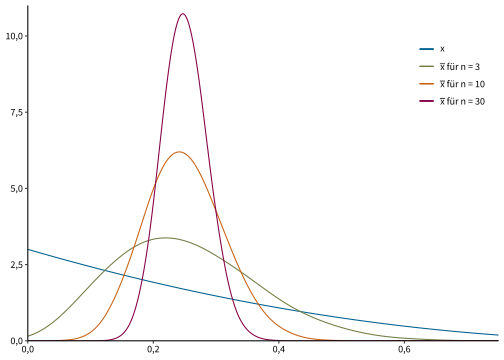
\includegraphics[width=.6\linewidth]{Skript_Statistik_2021_files/figure-latex/beta-1} 

}

\caption{Stichprobenverteilung bei nicht normalverteilter Population}\label{fig:beta}
\end{figure}

In der Praxis gilt die Faustregel: Ab einer Stichprobengröße von \(n=30\) können wir statistische Verfahren anwenden, die von einer theoretischen Normalverteilung von \(\bar{x}\) ausgehen -- und zwar \emph{unabhängig} von der Verteilung der Grundgesamtheit.

\hypertarget{punktschuxe4tzung}{%
\section{Punktschätzung}\label{punktschuxe4tzung}}

Bei statistischen Untersuchungen geht es oft darum, ausgehend von der empirischen Verteilung einer Stichprobe auf Parameter der Grundgesamtheit zu schließen.

Die Punktschätzung (engl. \emph{point estimation}) ist dabei eine vergleichsweise einfache und intuitive Vorgehensweise.

\hypertarget{punktschuxe4tzung-des-arithmetischen-mittels}{%
\subsection{Punktschätzung des arithmetischen Mittels}\label{punktschuxe4tzung-des-arithmetischen-mittels}}

Wenn eine Stichprobe vorliegt, dann ist ihr arithmetisches Mittel (\(\bar{x}\)) als erwartungstreuer Punktschätzer der wahrscheinlichste Wert für das arithmetische Mittel der Grundgesamtheit (\(\mu\)). Es gilt

\[
\hat{\mu} = \bar{x}
\label{eq:muhat}
\]

wobei das \enquote{Dach} auf dem \(\mu\) dafür steht, dass es sich nur um eine Schätzung handelt.

Beispiel:

\begin{itemize}
\tightlist
\item
  Zehn Studierende der Humangeographie werden zufällig ausgewählt, um ihre Pendelzeit zum IG-Farben-Campus zu erfassen.
\item
  Die Angaben in Minuten lauten:
  \texttt{22\ 26\ 12\ 23\ 48\ 31\ 15\ 71\ 17\ 35}
\item
  Das arithmetische Mittel der Messreihe lässt sich -- wie in \protect\hyperlink{arithmetisches-mittel}{Sitzung~2} ausführlich besprochen -- berechnen: \(\bar{x}=30\)
\item
  Da es sich um eine erwartungstreue Schätzgröße (und eine valide Zufallsstichprobe) handelt, kann die durchschnittliche Pendelzeit \emph{aller} Studierenden der Humangeographie gemäß Gleichung~\eqref{eq:muhat} auf \(\hat{\mu}=\bar{x}=30\) Minuten geschätzt werden.
\end{itemize}

Gleichzeitig wissen wir jedoch, dass diese Punktschätzung des arithmetischen Mittels vermutlich nicht ganz präzise ist, sondern einem Standardfehler (\(\sigma_{\bar{x}}\)) unterliegt. Woher wissen wir, wie groß dieser Standardfehler ist (und wie unpräzise damit unsere Schätzung)?

\hypertarget{punktschuxe4tzung-der-varianz-und-der-standardabweichung}{%
\subsection{Punktschätzung der Varianz und der Standardabweichung}\label{punktschuxe4tzung-der-varianz-und-der-standardabweichung}}

Bei der Varianz einer Stichprobe \(s^2\) handelt es sich ebenfalls um einen erwartungstreuen Punktschätzer für die Varianz der Grundgesamtheit \(\sigma^2\).

Es gilt also

\[
\hat{\sigma^2} = s^2 \label{eq:varhat}
\]

und damit natürlich auch

\[
\hat{\sigma} = s \label{eq:sigmahat}
\]

\hypertarget{schuxe4tzung-des-standardfehlers}{%
\subsection{Schätzung des Standardfehlers}\label{schuxe4tzung-des-standardfehlers}}

Wir führen das obige Beispiel fort:

\begin{itemize}
\tightlist
\item
  Die Varianz der Stichprobe können wir berechnen: \(s^2\approx319{,}78\) (s.\protect\hyperlink{varianz}{Sitzung~2}).
\item
  Die Varianz der Grundgesamtheit kann also mit Gleichung~\eqref{eq:muhat} auch auf \(\hat{\sigma^2}=s^2\approx319{,}78\) geschätzt werden.
\item
  Analog können wir die Standardabweichung der Population auf \(\hat{\sigma}=s\approx17{,}88\) schätzen.
\item
  Den Standardfehler können wir mit diesem Schätzwert anhand Gleichung~\eqref{eq:4sd} berechnen. Allerdings benutzen wir statt \(\sigma_{\bar{x}}\) das Symbol \(s_{\bar{x}}\), da es sich um einen Schätzwert handelt:
\end{itemize}

\nopagebreak

\[
\begin{aligned}
s_{\bar{x}} &= \frac{s}{\sqrt{n}}\\[4pt]
&\approx \frac{17{,}88}{\sqrt{10}}\approx5{,}65
\end{aligned}
\]

Je größer die Stichprobe, desto genauer lassen sich also Parameter der Population schätzen. Die statistische Antwort auf die Frage, wie groß die Stichprobe denn sein müsse, lautet demnach zunächst immer: Möglichst groß!

Bemerkenswert ist jedoch, dass dabei die Größe der Grundgesamtheit (\(N\), im Beispiel die Anzahl aller Studierenden der Humangeographie) bei diesen Überlegungen überhaupt keine Rolle spielt.

\hypertarget{intervallschuxe4tzung}{%
\section{Intervallschätzung}\label{intervallschuxe4tzung}}

Um eine Intervallschätzung durchführen zu können, muss:

\begin{itemize}
\tightlist
\item
  die Standardabweichung der Grundgesamtheit \(\sigma\) bekannt und
\item
  die theoretische Verteilung von \(\bar{x}\) normalverteilt sein. Das bedeutet:

  \begin{itemize}
  \tightlist
  \item
    \emph{Entweder} es ist bekannt, dass die Grundgesamtheit normalverteilt ist
  \item
    \emph{Und/oder} die Stichprobengröße ist \(n\geq30\)
  \end{itemize}
\end{itemize}

Für das obige Beispiel der Pendelzeiten wissen wir nicht, wie die Verteilung der Grundgesamtheit aussieht, und die Stichprobengröße (\(n=10\)) ist kleiner als 30. Eine Intervallschätzung können wir hier also nicht durchführen!

Auch bei der Intervallschätzung (engl. \emph{interval estimation}) geht es darum, das arithmetische Mittel der Population (\(\mu\)) zu schätzen. Allerdings geben wir nicht einfach nur den wahrscheinlichsten Wert an, sondern einen Bereich (ein \emph{Intervall}), in dem \(\mu\) mit einer bestimmten Wahrscheinlichkeit liegt.

Die Grundüberlegung ist dabei folgende:

\begin{itemize}
\tightlist
\item
  Wir haben eine \emph{empirische} Stichprobe vorliegen (und können ihren Mittelwert \(\bar{x}\) und ihre Standardabweichung \(s\) berechnen).
\item
  Wir wissen dass die \emph{theoretische} Verteilung aller möglichen Stichproben normalverteilt ist, und um den gesuchten Wert \(\mu\) symmetrisch ist.
\item
  Den Mittelwert unserer empirischen Stichprobe \(\bar{x}\) können wir uns als zufälligen Wert der theoretischen Stichprobenverteilung von \(\bar{x}\) vorstellen.
\item
  Wo genau in dieser theoretischen Verteilung wir mit unserem empirischen Wert \enquote{gelandet} sind, wissen wir nicht.
\item
  Wenn wir den Wert \(\mu\) kennen würden, könnten wir (mit den Methoden aus \protect\hyperlink{wahrscheinlichkeitsrechnung-mit-standardnormalverteilung}{Sitzung~3}) die Wahrscheinlichkeit für einen beliebeigen Bereich angeben, in den ein zufälliges \(\bar{x}\) fällt.
\item
  Der entscheidende Trick: Weil die Normalverteilung symmetrisch ist, sind diese Wahrscheinlichkeiten analog anzuwenden auf die Bereiche einer konstruierten Verteilung mit gleichem \(\sigma_{\bar{x}}\) um unser \(\bar{x}\), in die der wirkliche Wert \(\mu\) fällt. (s. Abbildung~\ref{fig:double}).
\end{itemize}

\begin{figure}[!h]

{\centering 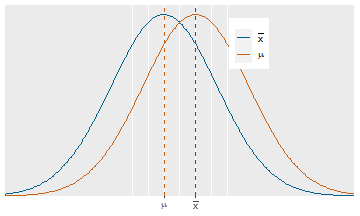
\includegraphics[width=.6\linewidth]{Skript_Statistik_2021_files/figure-latex/double-1} 

}

\caption{Konstruierte Verteilung um $\bar{x}$}\label{fig:double}
\end{figure}

Dabei heißt der Bereich Konfidenzintervall (engl. \emph{confidence interval}), und seine Breite wird mit \(\textrm{KIB}\) abgekürzt. Die Wahrscheinlichkeit, dass wir mit unserer Schätzung \emph{außerhalb} des Konfidenzintervalls liegen wird mit \(\alpha\) gekennzeichnet. Ein 95\%-Konfidenzintervall hat also ein \(\alpha\) von 0,05 (s. Abbildung~\ref{fig:konf}).

\begin{figure}[!h]

{\centering 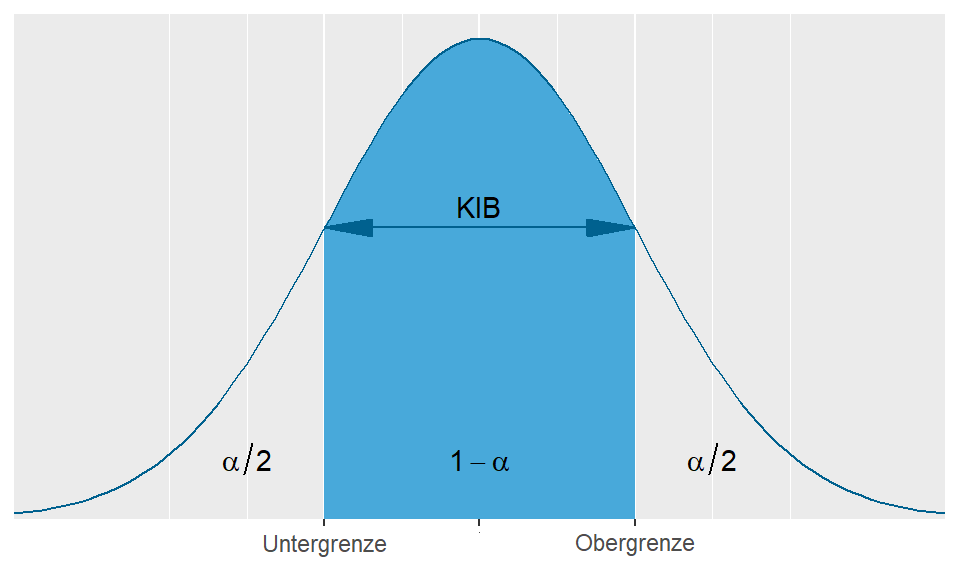
\includegraphics[width=.6\linewidth]{Skript_Statistik_2021_files/figure-latex/konf-1} 

}

\caption{Konfidenzintervall}\label{fig:konf}
\end{figure}

\begin{table}

\caption{\label{tab:tab}Jahresniederschlag in Hessen}
\centering
\begin{tabular}[t]{rr}
\toprule
Jahr & Niederschlag (l/m²)\\
\midrule
2011 & 855,3\\
2012 & 839,5\\
2013 & 850,6\\
2014 & 873,1\\
2015 & 858,3\\
2016 & 857,1\\
2017 & 861,4\\
\bottomrule
\end{tabular}
\end{table}

Ein Beispiel soll dies verdeutlichen: Wir wissen, dass die jährliche Niederschlagsmenge in Hessen normalverteilt ist mit \(\sigma=10{,}23\). Wir haben die Messwerte in Tabelle 1 erhoben und möchten den Mittelwert (\(\mu\)) per Intervallschätzung angeben.

Zunächst errechnen wir den Mittelwert unserer empirischen Stichprobe:

\nopagebreak

\[
\begin{aligned}
  \bar{x}&\approx856{,}47
\end{aligned}
\]

Dann errechnen wir anhand Gleichung~\eqref{eq:4sd} den Standardfehler der theoretischen Verteilung von \(\bar{x}\):

\nopagebreak

\[\begin{aligned}
\sigma_{\bar{x}}&=\frac{\sigma}{\sqrt{n}}\\[4pt]
           &\approx\frac{10{,}23}{\sqrt{7}}\approx3,86
\end{aligned}\]

\hypertarget{gesuchtes-alpha}{%
\subsection{\texorpdfstring{Gesuchtes \(\alpha\)}{Gesuchtes \textbackslash alpha}}\label{gesuchtes-alpha}}

Nun könnte eine Fragerichtung lauten: Wie groß ist die Wahrscheinlichkeit, dass der Mittelwert der Population \(\mu\) in einem Korridor von ± 5 l/m² um \(\bar{x}\) liegt?\footnote{Genau genommen ist das nicht ganz korrekt, \enquote{denn tatsächlich kann der Parameter nur innerhalb oder außerhalb des gefundenen Bereichs liegen. Die Wahrscheinlichkeit, dass ein Parameter in einen bestimmten Bereich fällt, ist damit entweder 0 oder 1.} (\protect\hyperlink{ref-bortz}{Bortz und Schuster 2010}: 93). Mathematisch korrekt müsste es heißen: \enquote{Die Wahrscheinlichkeit, dass \(\bar{x}\) zu einer Population gehört, deren Parameter \(\mu\) in diesem Bereich liegt\ldots{}}}

Gesucht ist bei einer Konfidenzintervallbreite von \(\textit{KIB}=10\) also die Wahrscheinlichkeit:

\nopagebreak

\[1-\alpha\approx P(851{,}47 < \mu < 861{,}47)\]

Generalisierend lässt sich schreiben:

\nopagebreak

\[
1-\alpha=P(x_{\alpha/2} < \mu < x_{(1-\alpha/2)})
\]

\nopagebreak

\ldots wobei \(x_{\alpha/2}\) die Untergrenze darstellt und \(x_{(1-\alpha/2)}\) die Obergrenze.

In \(z\)-Werten ausgedrückt:

\nopagebreak

\[
1-\alpha=P(z_{\alpha/2} < z_{\mu} < z_{(1-\alpha/2)})
\label{eq:konf}
\]

In \protect\hyperlink{wahrscheinlichkeitsrechnung-mit-standardnormalverteilung}{Sitzung~3} haben wir bereits gelernt, wie diese Wahrscheinlichkeit berechnet werden kann. Im Folgenden wird der Rechenweg noch einmal am Beispiel dargelegt.

\hypertarget{die-umstuxe4ndliche-variante}{%
\subsubsection{Die umständliche Variante}\label{die-umstuxe4ndliche-variante}}

Zunächst müssen wir die Intervallgrenzen in\(z\)-Werte umwandeln, um die Unter- bzw. Überschreitungswahrscheinlichkeiten ermitteln zu können. Die z-Transformation muss hier jedoch anhand des Standardfehlers \(\sigma_{\bar{x}}\) geschehen, da wir ja an der Stichprobenverteilung interessiert sind. Durch \(z\)-Transformation mit \(\bar{x}\) und dem Standardfehler \(\sigma_{\bar{x}}\) erhalten wir die standardisierten Intervallgrenzen.

Untergrenze:

\nopagebreak

\[\begin{aligned}
z_{\alpha/2} &= \frac{x_{\alpha/2}-\bar{x}}{\sigma_{\bar{x}}}\\[4pt]
&\approx\frac{851{,}47-856,47}{3,86}\approx-1,30
\end{aligned}\]

Obergrenze:

\nopagebreak

\[\begin{aligned}
z_{(1-\alpha/2)} &= \frac{x_{(1-\alpha/2)}-\bar{x}}{\sigma_{\bar{x}}}\\[4pt]
&\approx\frac{861{,}47-856,47}{3,86}\approx1,30
\end{aligned}\]

Es ist wenig überraschend, dass die \(z\)-transformierten Werte symmetrisch sind. Wir setzen in Gleichung~\eqref{eq:konf} ein:

\nopagebreak

\[1-\alpha\approx P(-1{,}30 <z_{\mu} < 1{,}30)\]

Dies lässt sich umformen in:

\nopagebreak

\[
1-\alpha\approx P(z_{\mu}<1{,}08) - P(z_{\mu}<-1{,}08) 
\]

Die jeweiligen Wahrscheinlichkeiten lassen sich in der Tabelle für \(p\)-Werte der Normalverteilung nachschauen (bzw. für den negativen \(z\)-Wert errechnen, s. \href{Formelsammlung\%20und\%20Wertetabellen.pdf}{Formelsammlung}):

\nopagebreak

\[
\begin{aligned}
1-\alpha&\approx 0,9032 - 0,0968\\
&=0,8064
\end{aligned}
\]

Die Wahrscheinlichkeit, dass \(\mu\) im Konfidenzintervalls 856,47 ± 5 l/m² liegt, beträgt also 80,64\%.

\hypertarget{die-schnelle-variante}{%
\subsubsection{Die schnelle Variante}\label{die-schnelle-variante}}

Wir können den \(z\)-Wert für die Obergrenze des Konfidenzintervalls ganz einfach ausrechnen, weil wir wissen, dass die Obergrenze um 5 größer ist als \(\bar{x}\) und dass \(z_{\bar{x}}=0\):

\nopagebreak

\[\begin{aligned}
z_{(1-\alpha/2)}&=\frac{5}{\sigma_{\bar{x}}}\\
&\approx\frac{5}{3,86}\\
&\approx1{,}30
\end{aligned}\]

Oberhalb dieses Werts liegt bekanntermaßen der Anteil \(\frac{\alpha}{2}\), woraus sich mit Blick auf die Tabelle ergibt:

\nopagebreak

\[\begin{aligned}
\frac{\alpha}{2}&=1-0,9032\\[4pt]
\alpha&=0,1936
\end{aligned}\]

\hypertarget{gesuchtes-konfidenzintervall}{%
\subsection{Gesuchtes Konfidenzintervall}\label{gesuchtes-konfidenzintervall}}

Eine weitere Möglichkeit der Fragestellung lautet: In welchem Bereich liegt das arithmetische Mittel \(\mu\) mit einer Wahscheinlichkeit von 90\%?

Vorgegeben ist also \(\alpha=0{,}1\), und gesucht sind die Unter- und die Obergrenze des Konfidenzintervalls.

Wir setzen ein:

\nopagebreak

\[\begin{aligned}
1-\alpha&=P(z_{\alpha/2} < z_{\mu} < z_{(1-\alpha/2)})\\[4pt]
0{,}9 &= P(z_{5\%} < z_{\mu} < z_{95\%})
\end{aligned}\]

Die entsprechenden \(z\)-Werte der Intervallgrenzen lassen sich (in umgekehrter Suchrichtung) aus der Tabelle ablesen:

\nopagebreak

\[\begin{aligned}
z_{5\%}&\approx-1{,}64\\[4pt]
z_{95\%}&\approx 1{,}64
\end{aligned}\]

Durch umgekehrte z-Transformation -- auch hier weider mit \(\bar{x}\) und \(\sigma_{\bar{x}}\) -- ergeben sich die Intervallgrenzen.

Untergrenze:

\nopagebreak

\[\begin{aligned}
x_{5\%} &= z_{5\%} \cdot \sigma_{\bar{x}} + \bar{x}\\[4pt]
&\approx -1{,}64 \cdot 3,86 + 856{,}47\\[4pt]
&\approx 850,14\\[6pt]
\end{aligned}\]

Obergrenze:

\nopagebreak

\[
\begin{aligned}
x_{95\%}&= z_{95\%} \cdot \sigma_{\bar{x}} + \bar{x}\\[4pt]
&\approx 1{,}64 \cdot 3,86 + 856{,}47\\[4pt]
&\approx 862,80
\end{aligned}\]

Auch hier gibt es wieder eine kleine Abkürzung: Aufgrund der Symmetrie unserer theoretischen Verteilung gilt für die Konfidenzintervallbreite generell:

\nopagebreak

\[
\frac{\mathit{KIB}}{2} = z_{(1-\alpha/2)} \cdot \sigma_{\bar{x}}
\label{eq:kib}
\]

Wir setzen einfach unsere Werte ein:

\nopagebreak

\[\begin{aligned}
\frac{\mathit{KIB}}{2} &= z_{95\%} \cdot s_{\bar{x}}\\[4pt]
&\approx1{,}64 \cdot 3,86\\[4pt]
&\approx 6,33
\end{aligned}\]

Die Intervallgrenzen ergeben sich dann trivial aus \(\bar{x} \pm \frac{\mathit{KIB}}{2}\).

\hypertarget{gesuchtes-n}{%
\subsection{\texorpdfstring{Gesuchtes \(n\)}{Gesuchtes n}}\label{gesuchtes-n}}

Eine letzte Fragerichtung lautet: Wie viele Messwerte müssten vorliegen, um den durchschnittlichen Niederschlag mit einem Konfidenzniveau von 99\% und einer Genauigkeit von ± 5 l/m² schätzen zu können?

Gegeben sind also das Konfidenzintervall und \(\alpha=0{,}01\), gesucht wird \(n\). Wir wissen, dass die Stichprobengröße \(n\) den Standardfehler \(\sigma_{\bar{x}}\) bestimmt. Also benutzen wir zunächst Gleichung~\eqref{eq:kib} und formen um:

\nopagebreak

\[\begin{aligned}
\frac{\mathit{KIB}}{2} &= z_{(1-\alpha/2)} \cdot \sigma_{\bar{x}}\\[4pt]
\sigma_{\bar{x}} &= \frac{\mathit{KIB}}{2\cdot z_{(1-\alpha/2)}} 
\end{aligned}\]

Durch Einsetzen und mit Blick auf die Tabelle erhalten wir:

\nopagebreak

\[\begin{aligned}
\sigma_{\bar{x}} &= \frac{10}{2\cdot z_{99{,}5\%}}\\[4pt]
 &\approx \frac{10}{2\cdot 2{,}58}\\[4pt]
 &\approx 1{,}94
\end{aligned}\]

Dieser Standardfehler \(\sigma_{\bar{x}}\approx1{,}94\) würde unseren Anforderungen genügen. Welches \(n\) ist nötig, um diesen Standardfehler zu erreichen? Wir formen Gleichung~\eqref{eq:4sd} um\ldots{}

\nopagebreak

\[\begin{aligned}
\sigma_{\bar{x}} &= \frac{\sigma}{\sqrt{n}}\\[4pt]
               n &= \Big(\frac{\sigma}{\sigma_{\bar{x}}}\Big)^2
\end{aligned}\]

\ldots und setzen den angestrebten Standardfehler sowie die Standardabweichung der Population (\(\sigma=10{,}23\)) ein:

\nopagebreak

\[
\begin{aligned}
n&=\Big(\frac{\sigma}{\sigma_{\bar{x}}}\Big)^2\\[4pt]
n&\approx\bigg(\frac{10{,}23}{1{,}94}\bigg)^2\\[4pt]
&\approx27{,}80
\end{aligned}
\]

Wir müssten also 28 Stichproben vorliegen haben.

\hypertarget{tipps-zur-vertiefung-3}{%
\section*{Tipps zur Vertiefung}\label{tipps-zur-vertiefung-3}}
\addcontentsline{toc}{section}{Tipps zur Vertiefung}

\begin{itemize}
\tightlist
\item
  YouTube-Kanal \enquote{Kurzes Tutorium Statistik}: \href{https://www.youtube.com/watch?v=DdwTa28W4Os}{Intervallschätzungen - Konfidenzintervalle}
\item
  Kapitel 6.2--6.4 in \protect\hyperlink{ref-bortz}{Bortz und Schuster} (\protect\hyperlink{ref-bortz}{2010})
\item
  Kapitel 8.1.1 -- 8.1.4 in \protect\hyperlink{ref-delange}{Lange und Nipper} (\protect\hyperlink{ref-delange}{2018})
\item
  Kapitel 8 in \protect\hyperlink{ref-klemm}{Klemm} (\protect\hyperlink{ref-klemm}{2002})
\item
  Kapitel 5.3.1 in \protect\hyperlink{ref-bahrenberg}{Bahrenberg, Giese und Nipper} (\protect\hyperlink{ref-bahrenberg}{2010})
\item
  \emph{English:} Kapitel 8 in \protect\hyperlink{ref-burt}{Burt und Barber} (\protect\hyperlink{ref-burt}{1996})
\end{itemize}

\hypertarget{uxfcbungsaufgaben-3}{%
\section*{Übungsaufgaben}\label{uxfcbungsaufgaben-3}}
\addcontentsline{toc}{section}{Übungsaufgaben}

Die folgenden Aufgaben sind zur eigenständigen Überprüfung Ihrer Lernleistung gedacht (als Vor- oder Nachbereitung der Vorlesung, oder als Klausurübung) und nicht etwa als Hausaufgabe.

\hypertarget{aufgabe-4-1}{%
\subsection{Aufgabe~4-1}\label{aufgabe-4-1}}

\protect\hyperlink{loesung-4-1}{zur~Lösung}

Eine Messreihe habe die Werte:

\begin{verbatim}
165  173  155  179  158  142
\end{verbatim}

\begin{enumerate}
\def\labelenumi{\alph{enumi})}
\tightlist
\item
  Führen Sie eine Punktschätzung für \(\mu\) und \(\sigma\) der Grundgesamtheit durch.
\item
  Welcher Standardfehler für \(\bar{x}\) ist zu erwarten?
\end{enumerate}

\hypertarget{aufgabe-4-2}{%
\subsection{Aufgabe~4-2}\label{aufgabe-4-2}}

\protect\hyperlink{loesung-4-2}{zur~Lösung}

Die Sonnenstunden auf einer Ferieninsel (pro Tag, im Jahresdurschnitt) sind annähernd normalverteilt mit einer Standardabweichung von vier Minuten. Der Mittelwert \(\mu\) ist unbekannt, es liegen neun Messwerte vor.

\begin{enumerate}
\def\labelenumi{\alph{enumi})}
\tightlist
\item
  Welcher Standardfehler für \(\bar{x}\) ist zu erwarten?
\item
  Welche Konfidenzintervallbreite korrespondiert mit einem Konfidenzniveau von 95\%?
\item
  Mit welchem Konfidenzniveau lässt sich \(\mu\) \enquote{auf die Minute genau} (± 30 Sekunden) schätzen?
\item
  Welche Stichprobengröße ist nötig um den Mittelwert mit einer Konfidenzintervallbreite von zwei Minuten und -niveau von 90\% zu schätzen?
\end{enumerate}

\hypertarget{aufgabe-4-3}{%
\subsection{Aufgabe~4-3}\label{aufgabe-4-3}}

\protect\hyperlink{loesung-4-3}{zur~Lösung}

Sie intressieren sich für das Durchschnittseinkommen (in EUR) der Haushalte eines Stadtteils. Die Varianz ist mit \(\sigma^2=4096\) bekannt. Eine Zufallsstichprobe von 40 befragten Haushalten weist einen Mittelwert von \(\bar{x}=2650\) auf.

\begin{enumerate}
\def\labelenumi{\alph{enumi})}
\tightlist
\item
  Wie lautet das 90\%-Konfidenzintervall?
\item
  Mit welcher Wahrscheinlichkeit liegt das Durchschnittseinkommen zwischen 2640 und 2660 EUR?
\end{enumerate}

\hypertarget{aufgabe-4-4}{%
\subsection{Aufgabe~4-4}\label{aufgabe-4-4}}

\protect\hyperlink{loesung-4-4}{zur~Lösung}

Es sei bekannt, dass die Lieferzeit eines Bauteils aus Übersee annähernd normalverteilt ist mit einer Standardabweichung von 11,5 Tagen.

Bei sieben Bestellvorgängen werden folgende Lieferzeiten festgestellt (in Tagen):

\[116{,}5\quad 94{,}5\quad101{,}5\quad109{,}0\quad125{,}0\quad112{,}5\quad100{,}5\]

Sie interessieren sich für die tatsächliche durchschnittliche Lieferzeit, von der Sie auch in Zukunft ausgehen können.

\begin{enumerate}
\def\labelenumi{\alph{enumi})}
\tightlist
\item
  Berechnen Sie das arithmetische Mittel der beobachteten Werte für die Lieferzeit.
\item
  Was ist der Standardfehler für die Stichprobenverteilung von \(\bar{x}\)?
\item
  Zwischen welchen Werten liegt die tatsächliche durchschnittliche Lieferzeit mit 95\% Wahrscheinlichkeit?
\item
  Wie viele zusätzliche Messungen müssten Sie vornehmen, um den tatsächlichen Mittelwert im selben Wertebereich zu 99\% verorten zu können?
\end{enumerate}

\hypertarget{formeln}{%
\chapter*{Formelsammlung und Wertetabellen}\label{formeln}}
\addcontentsline{toc}{chapter}{Formelsammlung und Wertetabellen}

Die Formelsammlung mit Wertetabellen liegt als PDF vor. So (oder ähnlich) formatiert würden Ihnen diese Informationen auch in einer Präsenzklausur zur Verfügung stehen. Ich empfehle deshalb, das Dokument herunterzuladen und auszudrucken -- so gewöhnen Sie sich gleich an das Format.

\href{Formelsammlung\%20und\%20Wertetabellen.pdf}{Als PDF herunterladen}

\hypertarget{luxf6sungen-der-uxfcbungsaufgaben}{%
\chapter*{Lösungen der Übungsaufgaben}\label{luxf6sungen-der-uxfcbungsaufgaben}}
\addcontentsline{toc}{chapter}{Lösungen der Übungsaufgaben}

\hypertarget{sitzung-1}{%
\section*{Sitzung 1}\label{sitzung-1}}
\addcontentsline{toc}{section}{Sitzung 1}

\hypertarget{loesung-1-1}{%
\subsection{Lösung~1-1}\label{loesung-1-1}}

\protect\hyperlink{aufgabe-1-1}{zur Aufgabenstellung}

-- keine Musterlösung --

\hypertarget{loesung-1-2}{%
\subsection{Lösung~1-2}\label{loesung-1-2}}

\protect\hyperlink{aufgabe-1-2}{zur Aufgabenstellung}

-- keine Musterlösungen --

\hypertarget{loesung-1-3}{%
\subsection{Lösung~1-3}\label{loesung-1-3}}

\protect\hyperlink{aufgabe-1-3}{zur Aufgabenstellung}

\begin{table}[H]
\centering
\begin{tabular}{lllll}
\toprule
\textbf{ } & \textbf{Variable} & \textbf{Skalenniveau} & \textbf{Variablentyp} & \textbf{Anmerkungen}\\
\midrule
a) & Lebensalter in Jahren & Verhältnisskala & diskret & ganze Zahlen vorausgesetzt\\
b) & Regenmenge in mm & Verhältnisskala & stetig & \\
c) & Güteklasse & Ordinalskala & qualitativ & \\
d) & Passagieraufkommen & Verhältnisskala & diskret & \\
e) & Baujahr & Intervallskala & diskret & \\
f) & Geschwindigkeit in km/h & Verhältnisskala & stetig & bei ganzzahligen Werten: diskret\\
g) & Sozialstatus (Unter-, Mittel und Oberschicht) & Ordinalskala & qualitativ & \\
h) & Temperatur in °F & Intervallskala & stetig & \\
i) & Fläche eines Bundeslands in km² & Verhältnisskala & stetig & \\
j) & Temperatur in K & Verhältnisskala & stetig & 0 K ist ein natürlicher Nullpunkt\\
k) & Einwohnerzahl & Verhältnisskala & diskret & \\
l) & Pegelstand & Intervallskala & stetig & willkürlicher Nullpunkt\\
m) & Staatsangehörigkeit & Nominalskala & qualitativ & \\
n) & Interesse an Statistik (gering bis hoch) & Ordinalskala & qualitativ & \\
o) & Klausurnote & Ordinalskala & qualitativ & wird jedoch oft metrisch verwendet\\
p) & Bodentyp & Nominalskala & qualitativ & \\
q) & Entfernung zum Stadtzentrum in km & Verhältnisskala & stetig & \\
r) & Körpergröße & Verhältnisskala & stetig & \\
s) & Kleidergröße (S bis XXL) & Ordinalskala & qualitativ & \\
t) & Monatliches Nettoeinkommen & Verhältnisskala & stetig & oder diskret für Cent-Beträge\\
\bottomrule
\end{tabular}
\end{table}

\hypertarget{loesung-1-4}{%
\subsection{Lösung~1-4}\label{loesung-1-4}}

\protect\hyperlink{aufgabe-1-4}{zur Aufgabenstellung}

\hypertarget{a-1}{%
\subsubsection{a)}\label{a-1}}

Die Werte sind im Bereich zwischen 3 und 210 Stunden. Eine Klassengröße von 25 Stunden bietet sich an, es sind jedoch auch andere Größen denkbar. Da die Variable diskret zu sein scheint, können die Klassengrenzen als ganze Zahlen angegeben werden.

\begin{table}[H]
\centering
\begin{tabular}{lr}
\toprule
\textbf{Wert $x_i$} & \textbf{Häufigkeit $f_i$}\\
\midrule
von 0 bis unter 25 h & 9\\
von 25 bis unter 50 h & 5\\
von 50 bis unter 75 h & 2\\
von 75 bis unter 100 h & 3\\
von 100 bis unter 125 h & 1\\
von 125 bis unter 150 h & 1\\
von 150 bis unter 175 h & 0\\
von 175 bis unter 200 h & 2\\
von 200 bis unter 225 h & 1\\
\bottomrule
\end{tabular}
\end{table}

\hypertarget{b-1}{%
\subsubsection{b)}\label{b-1}}

Das Resultat sollte je nach gewählter Klassengröße in etwa so aussehen:

\begin{center}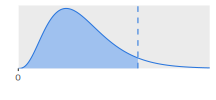
\includegraphics[width=.6\linewidth]{Skript_Statistik_2021_files/figure-latex/unnamed-chunk-33-1} \end{center}

\hypertarget{c-1}{%
\subsubsection{c)}\label{c-1}}

Die Verteilung ist unregelmäßig abfallend.

\hypertarget{loesung-1-5}{%
\subsection{Lösung~1-5}\label{loesung-1-5}}

\protect\hyperlink{aufgabe-1-5}{zur Aufgabenstellung}

Sind die folgenden Aussagen wahr oder unwahr?

\begin{enumerate}
\def\labelenumi{\alph{enumi})}
\tightlist
\item
  wahr
\item
  wahr
\item
  unwahr
\item
  wahr
\item
  unwahr
\item
  unwahr
\item
  wahr
\item
  wahr
\item
  unwahr
\item
  unwahr
\item
  wahr
\item
  wahr
\item
  unwahr
\item
  unwahr
\item
  unwahr
\item
  wahr
\item
  wahr
\item
  wahr
\end{enumerate}

\hypertarget{sitzung-2}{%
\section*{Sitzung 2}\label{sitzung-2}}
\addcontentsline{toc}{section}{Sitzung 2}

\hypertarget{loesung-2-1}{%
\subsection{Lösung~2-1}\label{loesung-2-1}}

\protect\hyperlink{aufgabe-2-1}{zur Aufgabenstellung}

\hypertarget{a-2}{%
\subsubsection{a)}\label{a-2}}

\begin{table}[H]
\centering
\begin{tabular}{ll}
\toprule
\textbf{Schritt} & \textbf{Lösung}\\
\midrule
Formel & $\bar{x}=\frac{\sum\limits_{i=1}^{n}x_{i}}{n}$\\
Einsetzen & $\bar{x}=\frac{356{,}00}{6}$\\
Ergebnis & $\bar{x}=59{,}33$\\
\bottomrule
\end{tabular}
\end{table}

\hypertarget{b-2}{%
\subsubsection{b)}\label{b-2}}

\begin{table}[H]
\centering
\begin{tabular}{ll}
\toprule
\textbf{Schritt} & \textbf{Lösung}\\
\midrule
Formel & $\bar{x}=\frac{\sum\limits_{i=1}^{n}x_{i}}{n}$\\
Einsetzen & $\bar{x}=\frac{2{,}08}{8}$\\
Ergebnis & $\bar{x}=0{,}26$\\
\bottomrule
\end{tabular}
\end{table}

\hypertarget{c-2}{%
\subsubsection{c)}\label{c-2}}

\begin{table}[H]
\centering
\begin{tabular}{ll}
\toprule
\textbf{Schritt} & \textbf{Lösung}\\
\midrule
Formel & $\bar{x}=\frac{\sum\limits_{i=1}^{n}x_{i}}{n}$\\
Einsetzen & $\bar{x}=\frac{8350{,}16}{10}$\\
Ergebnis & $\bar{x}=835{,}02$\\
\bottomrule
\end{tabular}
\end{table}

\hypertarget{loesung-2-2}{%
\subsection{Lösung~2-2}\label{loesung-2-2}}

\protect\hyperlink{aufgabe-2-2}{zur Aufgabenstellung}

\hypertarget{a-3}{%
\subsubsection{a)}\label{a-3}}

\begin{table}[H]
\centering
\begin{tabular}{ll}
\toprule
\textbf{Schritt} & \textbf{Lösung}\\
\midrule
Varianz: Formel & $s^2=\frac{\sum\limits_{i=1}^{n}(x_{i}-\bar{x})^2}{n-1}$\\
Varianz: Einsetzen & $s^2=\frac{1229{,}33}{5}$\\
Varianz: Ergebnis & $s^2=245{,}87$\\
Standardabweichung: Formel & $s=\sqrt{s^2}$\\
Standardabweichung: Einsetzen & $s=\sqrt{245{,}87}$\\
Varianz: Ergebnis & $s\approx15{,}68$\\
\bottomrule
\end{tabular}
\end{table}

\hypertarget{b-3}{%
\subsubsection{b)}\label{b-3}}

\begin{table}[H]
\centering
\begin{tabular}{ll}
\toprule
\textbf{Schritt} & \textbf{Lösung}\\
\midrule
Varianz: Formel & $s^2=\frac{\sum\limits_{i=1}^{n}(x_{i}-\bar{x})^2}{n-1}$\\
Varianz: Einsetzen & $s^2=\frac{1{,}63}{7}$\\
Varianz: Ergebnis & $s^2=0{,}23$\\
Standardabweichung: Formel & $s=\sqrt{s^2}$\\
Standardabweichung: Einsetzen & $s=\sqrt{0{,}23}$\\
Varianz: Ergebnis & $s\approx0{,}48$\\
\bottomrule
\end{tabular}
\end{table}

\hypertarget{c-3}{%
\subsubsection{c)}\label{c-3}}

\begin{table}[H]
\centering
\begin{tabular}{ll}
\toprule
\textbf{Schritt} & \textbf{Lösung}\\
\midrule
Varianz: Formel & $s^2=\frac{\sum\limits_{i=1}^{n}(x_{i}-\bar{x})^2}{n-1}$\\
Varianz: Einsetzen & $s^2=\frac{95338{,}94}{9}$\\
Varianz: Ergebnis & $s^2=10593{,}21$\\
Standardabweichung: Formel & $s=\sqrt{s^2}$\\
Standardabweichung: Einsetzen & $s=\sqrt{10593{,}21}$\\
Varianz: Ergebnis & $s\approx102{,}92$\\
\bottomrule
\end{tabular}
\end{table}

\hypertarget{loesung-2-3}{%
\subsection{Lösung~2-3}\label{loesung-2-3}}

\protect\hyperlink{aufgabe-2-3}{zur Aufgabenstellung}

\hypertarget{a-4}{%
\subsubsection{a)}\label{a-4}}

Die geordnete Liste ist:

\begin{verbatim}
1 1 1 2 2 2 2 3 3 4 4 5 7
\end{verbatim}

Für das arithmetische Mittel und die Varianz ist diese Tabelle hilfreich:

\begin{table}[H]
\centering
\begin{tabular}{llllll}
\toprule
\textbf{$x_i$} & \textbf{$f_i$} & \textbf{$f_i\cdot x_i$} & \textbf{$(x_i-\bar{x})$} & \textbf{$(x_i-\bar{x})^2$} & \textbf{$f_i\cdot(x_i-\bar{x})^2$}\\
\midrule
1 & 3 & 3 & -1,85 & 3,41 & 10,22\\
2 & 4 & 8 & -0,85 & 0,72 & 2,86\\
3 & 2 & 6 & 0,15 & 0,02 & 0,05\\
4 & 2 & 8 & 1,15 & 1,33 & 2,66\\
5 & 1 & 5 & 2,15 & 4,64 & 4,64\\
7 & 1 & 7 & 4,15 & 17,25 & 17,25\\
\bottomrule
\end{tabular}
\end{table}

Der häufigste Wert (und damit der Modalwert) ist 2.

Die Stichprobengröße ist ungerade (\(n=13\)), daher ist der Median: \[x_{(\frac{n+1}{2})} = x_{(7)} = 2\]

Das arithmetische Mittel berechnet sich einfacher mit den Werten aus der Tabelle:

\[\bar{x}={\displaystyle\frac{\sum\limits_{x=1}^nx_i}{n}}=\frac{3+8+6+8+5+6}{13}=\frac{37}{13}\approx2.85\]

\hypertarget{b-4}{%
\subsubsection{b)}\label{b-4}}

Die Spannweite ist: \[R=x_{(n)}-x_{(1)}=7-1=6\]

Der Quartilsabstand ist: \[\mathit{IQR}=Q_3-Q_1=4-2=2\]

Für die Varianz bieten sich ebenfalls die Tabellenwerte an: \[s^2=\frac{\sum\limits_{x=1}^n(x_i-\bar{x})^2}{n-1}\approx\frac{10,22+ 2,86+ 0,05+ 2,66+ 4,64+17,25}{13-1}=\frac{37,68}{12}=3.14\]

Schließlich ist die Standardabweichung: \[s=\sqrt{s^2}\approx\sqrt{3,14}\approx1,77\]

\hypertarget{c-4}{%
\subsubsection{c)}\label{c-4}}

Da der untere Angelpunkt und der Median zusammenfallen, sieht der Boxplot etwas ungewöhnlich aus:

\begin{center}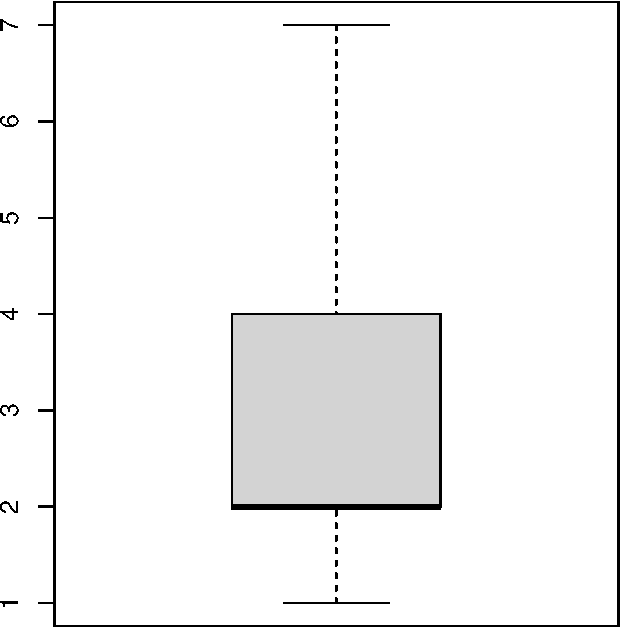
\includegraphics[width=.6\linewidth]{Skript_Statistik_2021_files/figure-latex/unnamed-chunk-43-1} \end{center}

\hypertarget{loesung-2-4}{%
\subsection{Lösung~2-4}\label{loesung-2-4}}

\protect\hyperlink{aufgabe-2-4}{zur Aufgabenstellung}

\hypertarget{a-5}{%
\subsubsection{a)}\label{a-5}}

Für den Quartilsabstand brauchen wir den Klassendurchschnitt und kumulative Häufigkeiten:

\begin{table}[H]
\centering
\begin{tabular}{lrrr}
\toprule
\textbf{$x$} & \textbf{$k_i$} & \textbf{$f_i$} & \textbf{$f_{kum}$}\\
\midrule
von 75 bis unter 77,5 cm & 76,25 & 1 & 1\\
von 77,5 bis unter 80 cm & 78,75 & 0 & 1\\
von 80 bis unter 82,5 cm & 81,25 & 3 & 4\\
von 82,5 bis unter 85 cm & 83,75 & 5 & 9\\
von 85 bis unter 87,5 cm & 86,25 & 7 & 16\\
von 87,5 bis unter 90 cm & 88,75 & 14 & 30\\
von 90 bis unter 92,5 cm & 91,25 & 9 & 39\\
von 92,5 bis unter 95 cm & 93,75 & 2 & 41\\
von 95 bis unter 97,5 cm & 96,25 & 2 & 43\\
\bottomrule
\end{tabular}
\end{table}

Bei \(n=43\) ist \(Q_1=\frac{x_{(11)}+x_{(12)}}{2}\) und \(Q_3=\frac{x_{(32)}+x_{(33)}}{2}\).

Aus der Tabelle mit kumulativen Häufigkeiten können wir \(Q_1=86{,}25\) und \(Q_3=91{,}25\) ablesen.

Der Quartilsabstand beträgt dann

\[\begin{aligned}
\mathit{IQR}&=Q_3-Q_1\\
            &=91{,}25-86{,}25\\
            &=5
\end{aligned}\]

\hypertarget{b-5}{%
\subsubsection{b)}\label{b-5}}

Um die Berechnung des arithmetischen Mittels zu vereinfachen berechnen wir den Klassendurchschnitt und Zwischensummen:

\begin{table}[H]
\centering
\begin{tabular}{lrrrr}
\toprule
\textbf{$x$} & \textbf{$k_i$} & \textbf{$f_i$} & \textbf{$f_{kum}$} & \textbf{$f_i \cdot k_i$}\\
\midrule
von 75 bis unter 77,5 cm & 76,25 & 1 & 1 & 76,25\\
von 77,5 bis unter 80 cm & 78,75 & 0 & 1 & 0,00\\
von 80 bis unter 82,5 cm & 81,25 & 3 & 4 & 243,75\\
von 82,5 bis unter 85 cm & 83,75 & 5 & 9 & 418,75\\
von 85 bis unter 87,5 cm & 86,25 & 7 & 16 & 603,75\\
von 87,5 bis unter 90 cm & 88,75 & 14 & 30 & 1242,50\\
von 90 bis unter 92,5 cm & 91,25 & 9 & 39 & 821,25\\
von 92,5 bis unter 95 cm & 93,75 & 2 & 41 & 187,50\\
von 95 bis unter 97,5 cm & 96,25 & 2 & 43 & 192,50\\
\bottomrule
\end{tabular}
\end{table}

Die Summen für das arithmetische Mittel entnehmen wir dann einfach der letzten Spalte:

\[\begin{aligned}
  \bar{x}&=\frac{\sum\limits_{i=1}^nx_i}{n} \\
         &=\frac{76{,}25+ 243{,}75+ 418{,}75+ 603{,}75+1242{,}50+ 821{,}25+ 187{,}50+ 192{,}50}{43} \\
         &=\frac{3786{,}25}{43} \\
         &\approx88{,}05
\end{aligned}\]

\hypertarget{c-5}{%
\subsubsection{c)}\label{c-5}}

Für die Varianz erweitern wir die Tabelle:

\begin{table}[H]
\centering
\begin{tabular}{lrrrrr}
\toprule
\textbf{$x_i$} & \textbf{$k_i$} & \textbf{$f_i$} & \textbf{$(k_i - \bar{x})$} & \textbf{$(k_i - \bar{x})^2$} & \textbf{$f_i \cdot (k_i - \bar{x})^2$}\\
\midrule
von 75 bis unter 77,5 cm & 76,25 & 1 & -11,8 & 139,24 & 139,24\\
von 77,5 bis unter 80 cm & 78,75 & 0 & -9,3 & 86,49 & 0,00\\
von 80 bis unter 82,5 cm & 81,25 & 3 & -6,8 & 46,24 & 138,72\\
von 82,5 bis unter 85 cm & 83,75 & 5 & -4,3 & 18,49 & 92,45\\
von 85 bis unter 87,5 cm & 86,25 & 7 & -1,8 & 3,24 & 22,68\\
von 87,5 bis unter 90 cm & 88,75 & 14 & 0,7 & 0,49 & 6,86\\
von 90 bis unter 92,5 cm & 91,25 & 9 & 3,2 & 10,24 & 92,16\\
von 92,5 bis unter 95 cm & 93,75 & 2 & 5,7 & 32,49 & 64,98\\
von 95 bis unter 97,5 cm & 96,25 & 2 & 8,2 & 67,24 & 134,48\\
\bottomrule
\end{tabular}
\end{table}

Die Varianz beträgt:

\[\begin{aligned}
  s^2&=\frac{\sum\limits_{i=1}^{n}(x_{i}-\bar{x})^2}{n-1} \\
     &=\frac{139{,}24+138{,}72+ 92{,}45+ 22{,}68+  6{,}86+ 92{,}16+ 64{,}98+134{,}48}{43-1}\\
     &=\frac{691{,}57}{42}\\
     &\approx{16{,}47}
\end{aligned}\]

\hypertarget{d}{%
\subsubsection{d)}\label{d}}

Somit beträgt die Standardabweichung

\[\begin{aligned}
  s&=\sqrt{s^2}\\
   &\approx\sqrt{16{,}47}\\
   &\approx4{,}06
\end{aligned}\]

\hypertarget{loesung-2-5}{%
\subsection{Lösung~2-5}\label{loesung-2-5}}

\protect\hyperlink{aufgabe-2-5}{zur Aufgabenstellung}

\hypertarget{a-6}{%
\subsubsection{a)}\label{a-6}}

\begin{table}[H]
\centering
\begin{tabular}{ll}
\toprule
\textbf{Schritt} & \textbf{Lösung}\\
\midrule
Formel & $\bar{x}=\frac{\sum\limits_{i=1}^{n}x_{i}}{n}$\\
Einsetzen & $\bar{x}=\frac{511{,}00}{6}$\\
Ergebnis & $\bar{x}=85{,}17$\\
Einsetzen & $\bar{y}=\frac{446{,}00}{6}$\\
Ergebnis & $\bar{y}=74{,}33$\\
Antwortsatz & Die Ziegelei weist im Mittel die größere Passant\*innenzahl auf.\\
\bottomrule
\end{tabular}
\end{table}

\hypertarget{b-6}{%
\subsubsection{b)}\label{b-6}}

\begin{table}[H]
\centering
\begin{tabular}{ll}
\toprule
\textbf{Schritt} & \textbf{Lösung}\\
\midrule
Formel & $\mathit{IQR}=Q_3-Q_1$\\
Einsetzen & $\mathit{IQR}_x=91-77$\\
Ergebnis & $\mathit{IQR}_x=14$\\
Einsetzen & $\mathit{IQR}_y=103-51$\\
Ergebnis & $\mathit{IQR}_y=52$\\
Antwortsatz & Das Möbellager hat den größeren Quartilsabstand für die Passant\*innenzahl.\\
\bottomrule
\end{tabular}
\end{table}

\hypertarget{loesung-2-6}{%
\subsection{Lösung~2-6}\label{loesung-2-6}}

\protect\hyperlink{aufgabe-2-6}{zur Aufgabenstellung}

\hypertarget{a-7}{%
\subsubsection{a)}\label{a-7}}

Es gibt eine Hierarchie der Werte (Ordinal-), sinnvolle Abstände (Intervall-) und einen sinnvollen Nullpunkt (Verhältnis-). Deshalb sind die angegebenen Werte als verhältnisskaliert zu verstehen.

\hypertarget{b-7}{%
\subsubsection{b)}\label{b-7}}

Klassen könnten z.~B. wie in der folgenden Tabelle gewählt werden. Um die Berechnung des arithmetischen Mittels zu vereinfachen berechnen wir gleich den Klassendurchschnitt und Zwischensummen:

\begin{table}[H]
\centering
\begin{tabular}{lrrrr}
\toprule
\textbf{$x$} & \textbf{$k_i$} & \textbf{$f_i$} & \textbf{$f_{kum}$} & \textbf{$f_i \cdot k_i$}\\
\midrule
von 300 bis unter 400 mm & 350 & 4 & 4 & 1400\\
von 400 bis unter 500 mm & 450 & 9 & 13 & 4050\\
von 500 bis unter 600 mm & 550 & 4 & 17 & 2200\\
von 600 bis unter 700 mm & 650 & 2 & 19 & 1300\\
von 700 bis unter 800 mm & 750 & 1 & 20 & 750\\
\bottomrule
\end{tabular}
\end{table}

\hypertarget{c-6}{%
\subsubsection{c)}\label{c-6}}

Der Modalwert der so klassierten Stichprobe ist die Klasse von 400 bis unter 500 mm und kann auch mit dem Klassenmittelwert 450 mm angegeben werden.

\hypertarget{d-1}{%
\subsubsection{d)}\label{d-1}}

Bei \(n=20\) ist \(Q_1=\frac{x_{(5)}+x_{(6)}}{2}\) und \(Q_3=\frac{x_{(15)}+x_{(16)}}{2}\).

Aus einer geordneten Liste könnten wir also

\[\begin{aligned}
Q_1&=\frac{x_{(5)}+x_{(6)}}{2}\\
   &=\frac{421{,}36+433{,}01}{2}\\
   &\approx427{,}19
\end{aligned}\]

und

\[\begin{aligned}
Q_3&=\frac{x_{(15)}+x_{(16)}}{2}\\
   &=\frac{527{,}75+235{,}12}{2}\\
   &\approx531{,}44
\end{aligned}\]

bestimmen.

Wenn uns nur die klassierte Verteilung zur Verfügung steht oder wenn der Datensatz besonders unübersichtlich ist, ist es auch legitim, aus der kumulativen Häufigkeit \(Q_1=450\) und \(Q_3=550\) für die klassierte Verteilung abzulesen.

Je nachdem beträgt der Quartilsabstand \(\mathit{IQR}=Q_3-Q_1\) dann 104,24 oder 100 mm.

\hypertarget{e}{%
\subsubsection{e)}\label{e}}

Die Summen für das arithmetische Mittel entnehmen wir der letzten Spalte der Wertetabelle:

\[\begin{aligned}
  \bar{x}&=\frac{\sum\limits_{i=1}^nx_i}{n} \\
         &=\frac{1400+4050+2200+1300+750}{20} \\
         &=\frac{9700}{20} \\
         &\approx485
\end{aligned}\]

\hypertarget{f}{%
\subsubsection{f)}\label{f}}

Für die Standardabweichung erweitern wir die Tabelle:

\begin{table}[H]
\centering
\begin{tabular}{lrrrrr}
\toprule
\textbf{$x_i$} & \textbf{$k_i$} & \textbf{$f_i$} & \textbf{$(k_i - \bar{x})$} & \textbf{$(k_i - \bar{x})^2$} & \textbf{$f_i \cdot (k_i - \bar{x})^2$}\\
\midrule
von 300 bis unter 400 mm & 350 & 4 & -135 & 18225 & 72900\\
von 400 bis unter 500 mm & 450 & 9 & -35 & 1225 & 11025\\
von 500 bis unter 600 mm & 550 & 4 & 65 & 4225 & 16900\\
von 600 bis unter 700 mm & 650 & 2 & 165 & 27225 & 54450\\
von 700 bis unter 800 mm & 750 & 1 & 265 & 70225 & 70225\\
\bottomrule
\end{tabular}
\end{table}

Die Varianz beträgt:

\[\begin{aligned}
  s^2&=\frac{\sum\limits_{i=1}^{n}(x_{i}-\bar{x})^2}{n-1} \\
     &=\frac{72900+11025+16900+54450+70225}{20-1}\\
     &=\frac{225500}{19}\\
     &\approx{11868{,}42}
\end{aligned}\]

Somit beträgt die Standardabweichung

\[\begin{aligned}
  s&=\sqrt{s^2}\\
   &\approx\sqrt{11868{,}42}\\
   &\approx108{,}94
\end{aligned}\]

\hypertarget{g}{%
\subsubsection{g)}\label{g}}

Auch der Boxplot lässt sich anhand der klassierten Werte zeichnen:

\begin{center}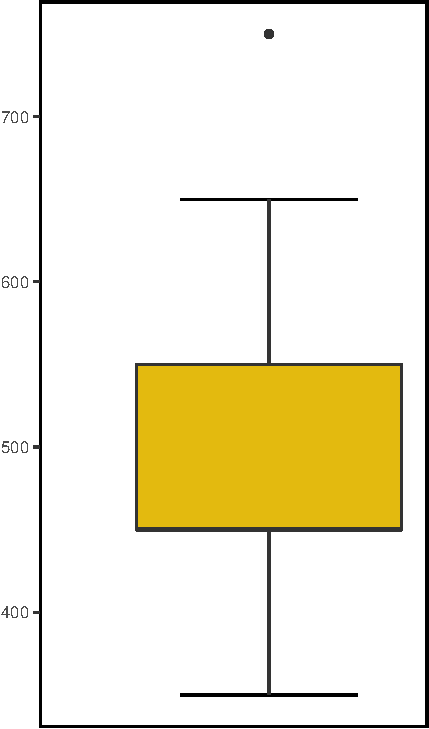
\includegraphics[width=0.35\linewidth]{Skript_Statistik_2021_files/figure-latex/solve_2_6_g-1} \end{center}

\hypertarget{sitzung-3}{%
\section*{Sitzung 3}\label{sitzung-3}}
\addcontentsline{toc}{section}{Sitzung 3}

\hypertarget{loesung-3-1}{%
\subsection{Lösung~3-1}\label{loesung-3-1}}

\protect\hyperlink{aufgabe-3-1}{zur Aufgabenstellung}

\hypertarget{a-8}{%
\subsubsection{a)}\label{a-8}}

Zunächst brauchen wir das arithmetische Mittel:

\begin{table}[H]
\centering
\begin{tabular}{ll}
\toprule
\textbf{Schritt} & \textbf{Musterlösung}\\
\midrule
Formel & $\bar{x}=\frac{\sum\limits_{i=1}^{n}x_{i}}{n}$\\
Einsetzen & $\bar{x}=\frac{-170{,}47}{9}$\\
Ergebnis & $\bar{x}=-18{,}94$\\
\bottomrule
\end{tabular}
\end{table}

Und die Standardabweichung:

\begin{table}[H]
\centering
\begin{tabular}{ll}
\toprule
\textbf{Schritt} & \textbf{Lösung}\\
\midrule
Formel & $s=\sqrt{s^2}$\\
Einsetzen & $s=\sqrt{61{,}08}$\\
Ergebnis & $s\approx7{,}82$\\
\bottomrule
\end{tabular}
\end{table}

Dann lässt sich die Formel bestimmen:

\begin{table}[H]
\centering
\begin{tabular}{ll}
\toprule
\textbf{Schritt} & \textbf{Musterlösung}\\
\midrule
Formel & $z_{i} = \frac{x_{i} - \bar{x}}{s}$\\
Einsetzen & $z_{i} = \frac{x_{i} +18{,}94}{7{,}82}$\\
\bottomrule
\end{tabular}
\end{table}

Und schließlich die einzelnen Werte berechnen. Hier sind die Berechnungen zum Prüfen ausformuliert, das wird in der Klausur nicht für jeden Wert erwartet.

\begin{table}[H]
\centering
\begin{tabular}{rl}
\toprule
\textbf{$x_i$} & \textbf{Berechnung}\\
\midrule
-16,93 & $z_{1}=\frac{-16{,}93+18{,}94}{7{,}82}\approx0{,}26$\\
-16,09 & $z_{2}=\frac{-16{,}09+18{,}94}{7{,}82}\approx0{,}36$\\
-10,97 & $z_{3}=\frac{-10{,}97+18{,}94}{7{,}82}\approx1{,}02$\\
-3,77 & $z_{4}=\frac{-3{,}77+18{,}94}{7{,}82}\approx1{,}94$\\
-25,55 & $z_{5}=\frac{-25{,}55+18{,}94}{7{,}82}\approx-0{,}85$\\
-20,57 & $z_{6}=\frac{-20{,}57+18{,}94}{7{,}82}\approx-0{,}21$\\
-23,61 & $z_{7}=\frac{-23{,}61+18{,}94}{7{,}82}\approx-0{,}60$\\
-25,90 & $z_{8}=\frac{-25{,}9+18{,}94}{7{,}82}\approx-0{,}89$\\
-27,08 & $z_{9}=\frac{-27{,}08+18{,}94}{7{,}82}\approx-1{,}04$\\
\bottomrule
\end{tabular}
\end{table}

\hypertarget{b-8}{%
\subsubsection{b)}\label{b-8}}

Zunächst die Standardabweichung:

\begin{table}[H]
\centering
\begin{tabular}{ll}
\toprule
\textbf{Schritt} & \textbf{Musterlösung}\\
\midrule
Formel & $s=\sqrt{s^2}$\\
Einsetzen & $s=\sqrt{13{,}02}$\\
Ergebnis & $s\approx3{,}61$\\
\bottomrule
\end{tabular}
\end{table}

Dann die Formel:

\begin{table}[H]
\centering
\begin{tabular}{ll}
\toprule
\textbf{Schritt} & \textbf{Musterlösung}\\
\midrule
Formel & $z_{i} = \frac{x_{i} - \bar{x}}{s}$\\
Umformen & $z_{i} = \frac{x_{i} - \bar{x}}{s}$\\
Einsetzen & $x_{i} = z_{i} \cdot 3{,}61 + 221{,}54$\\
\bottomrule
\end{tabular}
\end{table}

Schließlich die einzelnen Werte:

\begin{table}[H]
\centering
\begin{tabular}{rl}
\toprule
\textbf{$z_i$} & \textbf{Berechnung}\\
\midrule
0,90 & $x_{1} = 0{,}9 \cdot 3{,}61 + 221{,}54\approx224{,}79$\\
-1,40 & $x_{2} = -1{,}4 \cdot 3{,}61 + 221{,}54\approx216{,}49$\\
1,12 & $x_{3} = 1{,}12 \cdot 3{,}61 + 221{,}54\approx225{,}58$\\
-0,33 & $x_{4} = -0{,}33 \cdot 3{,}61 + 221{,}54\approx220{,}35$\\
2,22 & $x_{5} = 2{,}22 \cdot 3{,}61 + 221{,}54\approx229{,}55$\\
0,15 & $x_{6} = 0{,}15 \cdot 3{,}61 + 221{,}54\approx222{,}08$\\
2,87 & $x_{7} = 2{,}87 \cdot 3{,}61 + 221{,}54\approx231{,}90$\\
0,40 & $x_{8} = 0{,}4 \cdot 3{,}61 + 221{,}54\approx222{,}98$\\
-1,54 & $x_{9} = -1{,}54 \cdot 3{,}61 + 221{,}54\approx215{,}98$\\
0,13 & $x_{10} = 0{,}13 \cdot 3{,}61 + 221{,}54\approx222{,}01$\\
-0,17 & $x_{11} = -0{,}17 \cdot 3{,}61 + 221{,}54\approx220{,}93$\\
0,68 & $x_{12} = 0{,}68 \cdot 3{,}61 + 221{,}54\approx223{,}99$\\
\bottomrule
\end{tabular}
\end{table}

\hypertarget{loesung-3-2}{%
\subsection{Lösung~3-2}\label{loesung-3-2}}

\protect\hyperlink{aufgabe-3-2}{zur Aufgabenstellung}

\hypertarget{a-9}{%
\subsubsection{a)}\label{a-9}}

\(\sigma\) lässt sich berechnen durch:

\begin{table}[H]
\centering
\begin{tabular}{ll}
\toprule
\textbf{Schritt} & \textbf{Lösung}\\
\midrule
Formel & $\sigma=\sqrt{\sigma^2}$\\
Einsetzen & $\sigma=\sqrt{19{,}36}$\\
Lösung & $\sigma\approx4{,}40$\\
\bottomrule
\end{tabular}
\end{table}

Dann geht es zunächst darum, die \(x\)-Werte in \(z\)-Werte zu transformieren:

\begin{table}[H]
\centering
\begin{tabular}{lc}
\toprule
\textbf{Schritt} & \textbf{Lösung}\\
\midrule
Formel & $z_{i} = \frac{x_{i} - \mu}{\sigma}$\\
Einsetzen & $z_{i} = \frac{x_{i} - 32{,}2}{4{,}4}$\\
\bottomrule
\end{tabular}
\end{table}

Durch Einsetzen ergeben sich die folgenden Werte. (So ausführlich muss es in der Klausur nicht sein.)

\begin{table}[H]
\centering
\begin{tabular}{rc}
\toprule
\textbf{$x_i$} & \textbf{Berechnung}\\
\midrule
40,63 & $z_{1}=\frac{40{,}63-32{,}2}{4{,}4}\approx1{,}92$\\
20,77 & $z_{2}=\frac{20{,}77-32{,}2}{4{,}4}\approx-2{,}60$\\
33,41 & $z_{3}=\frac{33{,}41-32{,}2}{4{,}4}\approx0{,}27$\\
44,95 & $z_{4}=\frac{44{,}95-32{,}2}{4{,}4}\approx2{,}90$\\
41,91 & $z_{5}=\frac{41{,}91-32{,}2}{4{,}4}\approx2{,}21$\\
32,95 & $z_{6}=\frac{32{,}95-32{,}2}{4{,}4}\approx0{,}17$\\
\bottomrule
\end{tabular}
\end{table}

Für die positiven \(z\)-Werte können die Unterschreitungs­wahrscheinlichkeiten direkt in der Wertetabelle nachgeschaut werden. Für negative \(z\)-Werte gilt die Formel:

\[ P(z\leq -z_p) = 1-P(z \leq z_p) \]

Die Unterschreitungswerte ergeben:

\begin{table}[H]
\centering
\begin{tabular}{rllll}
\toprule
\textbf{$x_i$} & \textbf{$z_i$} & \textbf{Formel} & \textbf{Ergebnis} & \textbf{In Prozent}\\
\midrule
40,63 & 1,92 & $p=P(z \leq 1{,}92)$ & $p \approx 0{,}9726$ & 97,26\%\\
20,77 & -2,6 & $p=1-P(z \leq 2{,}6)$ & $p \approx 0{,}0047$ & 0,47\%\\
33,41 & 0,27 & $p=P(z \leq 0{,}27)$ & $p \approx 0{,}6064$ & 60,64\%\\
44,95 & 2,9 & $p=P(z \leq 2{,}9)$ & $p \approx 0{,}9981$ & 99,81\%\\
41,91 & 2,21 & $p=P(z \leq 2{,}21)$ & $p \approx 0{,}9864$ & 98,64\%\\
32,95 & 0,17 & $p=P(z \leq 0{,}17)$ & $p \approx 0{,}5675$ & 56,75\%\\
\bottomrule
\end{tabular}
\end{table}

\hypertarget{b-9}{%
\subsubsection{b)}\label{b-9}}

Es handelt sich um Überschreitungs­wahrscheinlichkeiten, aber aus der Tabelle lassen sich nur Unterschreitungswerte ablesen. Weil die Normalverteilung symmetrisch ist, gilt aber:

\[ P(x>x_p)=1-P(x\leq x_p)\]

So lässt sich jeweils sagen:

\begin{table}[H]
\centering
\begin{tabular}{rrlll}
\toprule
\textbf{Überschr. $p_{i}$} & \textbf{Unterschr. $(1-p_{1})$} & \textbf{Berechnung} & \textbf{....} & \textbf{Ergebnis}\\
\midrule
0,015 & 0,985 & $P(z \leq z_{1}) = 0{,}985$ &  & $z_{1} \approx 2{,}17$\\
0,025 & 0,975 & $P(z \leq z_{2}) = 0{,}975$ &  & $z_{2} \approx 1{,}96$\\
0,050 & 0,950 & $P(z \leq z_{3}) = 0{,}95$ &  & $z_{3} \approx 1{,}64$\\
0,130 & 0,870 & $P(z \leq z_{4}) = 0{,}87$ &  & $z_{4} \approx 1{,}13$\\
0,500 & 0,500 & $P(z \leq z_{5}) = 0{,}5$ &  & $z_{5} \approx 0{,}00$\\
0,900 & 0,100 & $P(z \leq -z_{6}) = 1-0{,}1 = 0{,}9$ & $-z_{6} \approx 1{,}28$ & $z_{6} \approx -1{,}28$\\
0,990 & 0,010 & $P(z \leq -z_{7}) = 1-0{,}01 = 0{,}99$ & $-z_{7} \approx 2{,}33$ & $z_{7} \approx -2{,}33$\\
0,995 & 0,005 & $P(z \leq -z_{8}) = 1-0{,}005 = 0{,}995$ & $-z_{8} \approx 2{,}58$ & $z_{8} \approx -2{,}58$\\
\bottomrule
\end{tabular}
\end{table}

Für die Rücktransformation gilt die Formel:

\[x_{i} = z_{i} \cdot \sigma + \mu\]

\begin{table}[H]
\centering
\begin{tabular}{lll}
\toprule
\textbf{$z_i$} & \textbf{Einsetzen} & \textbf{$x_i$}\\
\midrule
2,17 & $x_{1} = 2{,}17 \cdot 4{,}4 + 32{,}2$ & $x_{1}\approx41{,}75$\\
1,96 & $x_{2} = 1{,}96 \cdot 4{,}4 + 32{,}2$ & $x_{2}\approx40{,}82$\\
1,64 & $x_{3} = 1{,}64 \cdot 4{,}4 + 32{,}2$ & $x_{3}\approx39{,}42$\\
1,13 & $x_{4} = 1{,}13 \cdot 4{,}4 + 32{,}2$ & $x_{4}\approx37{,}17$\\
0 & $x_{5} = 0 \cdot 4{,}4 + 32{,}2$ & $x_{5}\approx32{,}20$\\
-1,28 & $x_{6} = -1{,}28 \cdot 4{,}4 + 32{,}2$ & $x_{6}\approx26{,}57$\\
-2,33 & $x_{7} = -2{,}33 \cdot 4{,}4 + 32{,}2$ & $x_{7}\approx21{,}95$\\
-2,58 & $x_{8} = -2{,}58 \cdot 4{,}4 + 32{,}2$ & $x_{8}\approx20{,}85$\\
\bottomrule
\end{tabular}
\end{table}

\hypertarget{c-7}{%
\subsubsection{c)}\label{c-7}}

Die mittleren 95\% der Werte liegen zwischen einem unteren Wert \(x_{2{,}5\%}\) (der zu 2,5\% unterschritten wird) und einem oberen Wert \(x_{97{,}5\%}\) (der zu 2,5\% überschritten wird).

Der obere \(z\)-Wert lässt sich leicht finden: \(z_{97{,}5\%} \approx 1{,}96\)

Durch Symmetrie wissen wir dann auch, dass: \(z_{2{,}5\%} \approx -1{,}96\)

Nun noch rückwärts transformieren:

\begin{table}[H]
\centering
\begin{tabular}{ll}
\toprule
\textbf{Schritt} & \textbf{Lösung}\\
\midrule
Formel & $x_{i} = z_{i} \cdot \sigma + \mu$\\
Untergrenze: Einsetzen & $x_{u} = -1{,}96 \cdot 4{,}4 + 32{,}2$\\
Untergrenze: Ergebnis & $x_{u}\approx23{,}58$\\
Obergrenze: Einsetzen & $x_{o} = 1{,}96 \cdot 4{,}4 + 32{,}2$\\
Obergrenze: Ergebnis & $x_{o}\approx40{,}82$\\
Antwortsatz & Die mittleren 95 Prozent der Werte liegen zwischen 23,58 und 40,82.\\
\bottomrule
\end{tabular}
\end{table}

\hypertarget{d-2}{%
\subsubsection{d)}\label{d-2}}

Es ist immer einfacher, mit Unterschreitungs­wahrscheinlichkeiten zu arbeiten. Zwischen 30 und 40 heißt auch: unter 40, aber nicht unter 30. Formal sieht das so aus:

\[P(30 < x \leq 40) = P(x \leq 40) - P(x \leq 30)\]

Diese Unterschreitungs­wahrscheinlichkeiten bestimmen wir wieder über die \(z\)-Transformation:

\begin{table}[H]
\centering
\begin{tabular}{ll}
\toprule
\textbf{Schritt} & \textbf{Lösung}\\
\midrule
Formel & $z_{i} = \frac{x_{i} - \mu}{\sigma}$\\
Untergrenze: $z$-Wert & $z_{u}=\frac{30-32{,}2}{4{,}4}\approx-0{,}50$\\
Untergrenze: Unterschr. & $p \approx 0{,}3085$\\
Obergrenze: $z$-Wert & $z_{o}=\frac{40-32{,}2}{4{,}4}\approx1{,}77$\\
Obergrenze: Unterschr. & $p \approx 0{,}9616$\\
Intervall & $P(30 < x \leq 40) = P(x \leq 40) - P(x \leq 30)$\\
Intervall einsetzen & $P(30 < x \leq 40) \approx P(z \leq 0{,}9616) - P(z \leq 0{,}3085)$\\
Intervall Ergebnis & $P(30 < x \leq 40) \approx 0{,}6531$\\
Antwortsatz & Ein zufälliger Wert der Verteilung liegt mit 65,31-prozentiger Wahrscheinlichkeit zwischen 30 und 40.\\
\bottomrule
\end{tabular}
\end{table}

\hypertarget{loesung-3-3}{%
\subsection{Lösung~3-3}\label{loesung-3-3}}

\protect\hyperlink{aufgabe-3-3}{zur Aufgabenstellung}

\hypertarget{a-10}{%
\subsubsection{a)}\label{a-10}}

Siehe b)

\hypertarget{b-10}{%
\subsubsection{b)}\label{b-10}}

Die Dichtefunktion mit kritischem Wert sollte in etwa so aussehen:

\begin{center}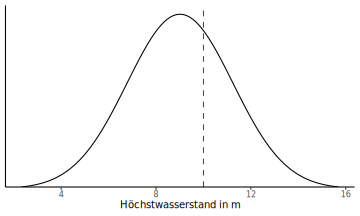
\includegraphics[width=.6\linewidth]{Skript_Statistik_2021_files/figure-latex/unnamed-chunk-70-1} \end{center}

\hypertarget{c-8}{%
\subsubsection{c)}\label{c-8}}

\[z_p=\frac{x_p- \mu}{\sigma} = \frac{10-9,01}{2,23}\approx0,44\]

\hypertarget{d-3}{%
\subsubsection{d)}\label{d-3}}

\[p=P(z<z_p)\approx P(z<0,44)\approx0,6700\]

Die Wahrscheinlichkeit, dass der Deich unbeschädigt bleibt, beträgt 67\%.

\hypertarget{loesung-3-4}{%
\subsection{Lösung~3-4}\label{loesung-3-4}}

\protect\hyperlink{aufgabe-3-4}{zur Aufgabenstellung}

\hypertarget{a-11}{%
\subsubsection{a)}\label{a-11}}

Die Übertretungswahrscheinlichkeit beträgt:

\[P(z>z_p) = 1- P(z<z_p) \approx 1-0,6700 = 0,3300 = 33\% \]

\hypertarget{b-11}{%
\subsubsection{b)}\label{b-11}}

Für \(x_p=12\) ergibt sich:

\[ z_p=\frac{x_p- \mu}{\sigma} = \frac{12-9,01}{2,23}\approx1,34 \]

Und für die Übertretungswahrscheinlichkeit:

\[P(z>z_p) = 1- P(z<z_p) \approx 1-0,9099 = 0,0901= 9,01\% \]

\hypertarget{c-9}{%
\subsubsection{c)}\label{c-9}}

Wir kennen \(P(x < 12)\approx0,9099\) aus Aufgabe 2 b) und \(P(x<10)\approx0,6700\) aus Aufgabe 1 d). Also rechnen wir:

\[P(10<x<12) = P(x<12) - P(x<10) \approx 0,9099 - 0,6700 = 0,2399\]

\hypertarget{d-4}{%
\subsubsection{d)}\label{d-4}}

Für die Obergrenze soll gelten: \(P(x<x_o) = 0,9\). Der Tabelle entnehmen wir \(z_o \approx 1,28\). Entsprechend ist \(z_u\approx-1,28\).

Die Umkehrung der \(z\)-Transformation ergibt:

\[\begin{aligned}
x_o&=z_o\cdot\sigma + \mu\approx1,28\cdot2,23 +9,01\approx11,86\\
x_u&=z_u\cdot\sigma + \mu\approx-1,28\cdot2.23 +9.01\approx6,16
\end{aligned}\]

Die mittleren 80\% der Werte liegen also zwichen 6,16 und 11,86~m.

\hypertarget{loesung-3-5}{%
\subsection{Lösung~3-5}\label{loesung-3-5}}

\protect\hyperlink{aufgabe-3-5}{zur Aufgabenstellung}

\hypertarget{a-12}{%
\subsubsection{a)}\label{a-12}}

\[p=P(x<x_p)=1-P(x>x_p)=1-\frac{1}{200}=1-0,005=0,995\]

\hypertarget{b-12}\approx2,58\]

\hypertarget{c-10}=z_{99,5\%}\cdot\sigma + \mu\approx2,58\cdot2,23+9,01\approx14,76\]

Der neue Deich muss 14,76~m hoch sein.

\hypertarget{loesung-3-6}{%
\subsection{Lösung~3-6}\label{loesung-3-6}}

\protect\hyperlink{aufgabe-3-6}{zur Aufgabenstellung}

\hypertarget{a-13}{%
\subsubsection{a)}\label{a-13}}

\begin{itemize}
\tightlist
\item
  \(z_p=1\) und \(P(z<1)\approx84,13\%\), also \(P(z>1)\approx15,87\%\)
\end{itemize}

\hypertarget{b-13}{%
\subsubsection{b)}\label{b-13}}

\begin{itemize}
\tightlist
\item
  \(z_p=-2\) und \(P(z<-2) = 1-P(z<2) \approx 1-0,9772 = 0,0228\)
\item
  Es kann also 2,28 Mal in 100 Jahren (oder: in etwa 2 von 100 Jahren, in weniger als 3 von 100 Jahren) mit weniger als 200~mm Regen gerechnet werden.
\end{itemize}

\hypertarget{c-11}{%
\subsubsection{c)}\label{c-11}}

\begin{itemize}
\tightlist
\item
  \(z_u=-2\) und \(P(z<z_u)\approx 0,0228\) (siehe b)
\item
  \(z_o=\frac{x_o- \mu}{\sigma}=\frac{550-400}{100}=1,5\) und \(P(z<z_o) \approx 0,9332\)
\item
  \(P(200 < x < 550) = P(x < 550) - P(x<200) \approx 91,04\%\)
\end{itemize}

\hypertarget{d-5}{%
\subsubsection{d)}\label{d-5}}

\begin{itemize}
\tightlist
\item
  Gesucht ist \(x_p\), für das gilt: \(P(x>x_p) = \frac{2}{100}=0,02\)
\item
  Daraus folgt: \(P(x<x_p) = 0,98\) und \(z_p\approx2,05\)
\item
  \(x_p = 605\)
\end{itemize}

\hypertarget{e-1}\approx -1,15\) und \(z_{87,5\%}= 1,15\)
\item
  Die mittleren 75\% liegen zwischen \(x_u=285\) und \(x_o=515\) mm.
\end{itemize}

\hypertarget{loesung-3-7}{%
\subsection{Lösung~3-7}\label{loesung-3-7}}

\protect\hyperlink{aufgabe-3-7}{zur Aufgabenstellung}

\textbf{Für die Ziegelei:}

\begin{table}[H]
\centering
\begin{tabular}{ll}
\toprule
\textbf{Schritt} & \textbf{Lösung}\\
\midrule
Varianz: Formel & $s^2=\frac{\sum\limits_{i=1}^{n}(x_{i}-\bar{x})^2}{n-1}$\\
Varianz: Einsetzen & $s^2_x=\frac{610{,}83}{5}$\\
Varianz: Ergebnis & $s^2_x=122{,}17$\\
Standardabweichung: Formel & $s=\sqrt{s^2}$\\
Standardabweichung: Ergebnis & $s_x\approx11{,}05$\\
Variationskoeffizient: Formel & $v=\frac{s}{|\bar{x}|}\cdot100\%\quad$\\
Variationskoeffizient: Einsetzen & $v\approx\frac{11{,}05}{85{,}17}\cdot100\%$\\
Variationskoeffizient: Ergebnis & $v \approx 12{,}97\%$\\
\bottomrule
\end{tabular}
\end{table}

\textbf{Für das Möbellager:}

\begin{table}[H]
\centering
\begin{tabular}{ll}
\toprule
\textbf{Schritt} & \textbf{Lösung}\\
\midrule
Varianz: Formel & $s^2=\frac{\sum\limits_{i=1}^{n}(x_{i}-\bar{x})^2}{n-1}$\\
Varianz: Einsetzen & $s^2_y=\frac{4015{,}33}{5}$\\
Varianz: Ergebnis & $s^2_y=803{,}07$\\
Standardabweichung: Formel & $s_y=\sqrt{s^2_y}$\\
Standardabweichung: Ergebnis & $s_y\approx28{,}34$\\
Variationskoeffizient: Formel & $v=\frac{s}{|\bar{x}|}\cdot100\%$\\
Variationskoeffizient: Einsetzen & $v\approx\frac{28{,}34}{74{,}33}\cdot100\%$\\
Variationskoeffizient: Ergebnis & $v \approx 38{,}13\%$\\
\bottomrule
\end{tabular}
\end{table}

\hypertarget{sitzung-4}{%
\section*{Sitzung 4}\label{sitzung-4}}
\addcontentsline{toc}{section}{Sitzung 4}

\hypertarget{loesung-4-1}{%
\subsection{Lösung~4-1}\label{loesung-4-1}}

\protect\hyperlink{aufgabe-4-1}{zur Aufgabenstellung}

\hypertarget{a-14}{%
\subsubsection{a)}\label{a-14}}

\(\mu = \bar{x} = 162\)

\(\sigma = s \approx 13{,}30\)

\hypertarget{b-14}{%
\subsubsection{b)}\label{b-14}}

\(\sigma_{\bar{x}} = \frac{\sigma}{\sqrt{n}}\approx\frac{13{,}30}{\sqrt{6}} \approx 5,42\)

\hypertarget{loesung-4-2}\cdot \sigma_{\bar{x}}\)

  \(\frac{\mathit{KIB}}{2}\approx 1{,}96 \cdot 1{,}33 \approx 2{,}61\)

  \(\mathit{KIB}=5{,}22\)
\item
  \(\frac{\mathit{KIB}}{2}=z_{(1-\alpha/2)} \cdot \sigma_{\bar{x}}\)

  \(z_{(1-\alpha/2)} = \frac{\mathit{KIB}}{2 \cdot \sigma_{\bar{x}}}\approx\frac{1}{2 \cdot 1{,}33}\approx0{,}38\)

  \(1-\frac{\alpha}{2} \approx 0{,}648\)

  \(-\frac{\alpha}{2} \approx 0{,}648 - 1\)

  \(\frac{\alpha}{2} \approx 0{,}352\)

  \(\alpha \approx 0{,}704\)

  Das Konfidenzniveau beträgt ca. 70,4\%.
\item
  \(\frac{\mathit{KIB}}{2} = z_{(1-\alpha/2)} \cdot \sigma_{\bar{x}}\)

  \(\sigma_{\bar{x}} = \frac{\mathit{KIB}}{2\cdot z_{95\%}}\)

  \(\sigma_{\bar{x}} = \frac{2}{2 \cdot z_{95\%}}\)

  \(\sigma_{\bar{x}} \approx \frac{2}{2 \cdot 1{,}65}\)

  \(\sigma_{\bar{x}} \approx 0{,}61\)

  \(\sigma_{\bar{x}}=\frac{\sigma}{\sqrt{n}}\)

  \(n = \big(\frac{\sigma}{\sigma_{\bar{x}}}\big)^2\)

  \(n \approx \big(\frac{4}{0{,}61}\big)^2\approx43\)
\end{enumerate}

\hypertarget{loesung-4-3}{%
\subsection{Lösung~4-3}\label{loesung-4-3}}

\protect\hyperlink{aufgabe-4-3}{zur Aufgabenstellung}

\hypertarget{a-15} \cdot \sigma_{\bar{x}}\)

\(\frac{\mathit{KIB}}{2}\approx 1{,}65 \cdot 10{,}12\approx16{,}70\)

\(\textrm{Untergrenze} = \bar{x} - \frac{\mathit{KIB}}{2} \approx 2650 - 16{,}70 = 2633{,}30\)

\(\textrm{Obergrenze} = \bar{x} + \frac{\mathit{KIB}}{2} \approx 2650 + 16{,}70 = 2666{,}70\)

\hypertarget{b-15}{%
\subsubsection{b)}\label{b-15}}

\(\mathit{KIB}=20\)

\(\frac{\mathit{KIB}}{2}=z_{(1-\alpha/2)} \cdot \sigma_{\bar{x}}\)

\(z_{(1-\alpha/2)}=\frac{\mathit{KIB}}{2\cdot \sigma_{\bar{x}}}\)

\(z_{(1-\alpha/2)}=\frac{20}{2 \cdot 10{,}12}\approx0{,}99\)

\(1-\frac{\alpha}{2}\approx0{,}8389\)

\(\alpha\approx 0{,}3222\)

Das Konfidenzniveau beträgt ca. 67,78\%.

\hypertarget{loesung-4-4}{%
\subsection{Lösung~4-4}\label{loesung-4-4}}

\protect\hyperlink{aufgabe-4-4}{zur Aufgabenstellung}

\hypertarget{a-16}{%
\subsubsection{a)}\label{a-16}}

\begin{table}[H]
\centering
\begin{tabular}{ll}
\toprule
\textbf{Schritt} & \textbf{Lösung}\\
\midrule
Formel & $\bar{x}=\frac{\sum\limits_{i=1}^{n}x_{i}}{n}$\\
Einsetzen & $\bar{x}=\frac{759{,}50}{7}$\\
Ergebnis & $\bar{x}=108{,}50$\\
\bottomrule
\end{tabular}
\end{table}

\hypertarget{b-16}{%
\subsubsection{b)}\label{b-16}}

\begin{table}[H]
\centering
\begin{tabular}{ll}
\toprule
\textbf{Schritt} & \textbf{Lösung}\\
\midrule
Formel & $\sigma_{\bar{x}}=\frac{\sigma}{\sqrt{n}}$\\
Einsetzen & $\sigma_{\bar{x}}=\frac{11{,}5}{\sqrt{7}}$\\
Ergebnis & $\sigma_{\bar{x}}\approx4{,}35$\\
\bottomrule
\end{tabular}
\end{table}

\hypertarget{c-12} \cdot \sigma_{\bar{x}} \approx 1{,}96 \cdot 4{,}35$\\
Ergebnis & $\frac{\mathit{KIB}}{2} \approx 8{,}53$\\
Antwortsatz & Die tatsächliche durchschnittliche Lieferzeit liegt mit 95\% Wahrscheinlichkeit zwischen 99,97 und 117,03 Tagen (108,5 $\pm$ 8,53).\\
\bottomrule
\end{tabular}
\end{table}

\hypertarget{d-6}} = 8{,}53 \cdot \frac{1}{2{,}58}$\\
Standardfehler: Ergebnis & $\sigma_{\bar{x}} \approx 3{,}31$\\
$n$: Formel & $\sigma_{\bar{x}}=\frac{\sigma}{\sqrt{n}}$\\
$n$: Umformen & $n=\Big(\frac{\sigma}{\sigma_{\bar{x}}}\Big)^2$\\
$n$: Einsetzen & $n=\Big(\frac{11{,}5}{3{,}31}\Big)^2$\\
$n$: Ergebnis & $n\approx12{,}07$\\
Antwortsatz & Es müssten 6 zusätzliche Messungen  vorgenommen werden (13 insgesamt).\\
\bottomrule
\end{tabular}
\end{table}

\hypertarget{quellenverzeichnis}{%
\chapter*{Quellenverzeichnis}\label{quellenverzeichnis}}
\addcontentsline{toc}{chapter}{Quellenverzeichnis}

\hypertarget{refs}{}
\begin{CSLReferences}{1}{0}
\leavevmode\vadjust pre{\hypertarget{ref-bahrenberg}{}}%
Bahrenberg, Gerhard, Ernst Giese und Josef Nipper. 2010. \emph{Statistische Methoden in der Geographie}. Bd. 1. Univariate und bivariate Statistik. Stuttgart: Bornträger.

\leavevmode\vadjust pre{\hypertarget{ref-benninghaus}{}}%
Benninghaus, Hans. 2007. \emph{Deskriptive Statistik. Eine Einführung für Sozialwissenschaftler}. Wiesbaden: VS Verlag.

\leavevmode\vadjust pre{\hypertarget{ref-bortz}{}}%
Bortz, Jürgen und Christof Schuster. 2010. \emph{Statistik für Human- und Sozialwissenschaftler}. Berlin: Springer.

\leavevmode\vadjust pre{\hypertarget{ref-burt}{}}%
Burt, James E. und Gerald M. Barber. 1996. \emph{Elementary statistics for geographers}. 2nd ed. New York: Guilford Press.

\leavevmode\vadjust pre{\hypertarget{ref-haseloff}{}}%
Haseloff, Otto W., Hans-Joachim Hoffmann, John H. Maindonald und W. John Braun. 1968. \emph{Kleines Lehrbuch der Statistik DAAG. Data Analysis and Graphics Data and Functions}. Berlin: de Gruyter.

\leavevmode\vadjust pre{\hypertarget{ref-klemm}{}}%
Klemm, Elmar. 2002. \emph{Einführung in die Statistik. Für die Sozialwissenschaften}. Wiesbaden: Westdeutscher Verlag.

\leavevmode\vadjust pre{\hypertarget{ref-delange}{}}%
Lange, Norbert de und Josef Nipper. 2018. \emph{Quantitative Methodik in der Geographie}. {UTB} Geographie, Methoden, Statistische Verfahren 4933. Paderborn: Ferdinand Schöningh.

\leavevmode\vadjust pre{\hypertarget{ref-daag}{}}%
Maindonald, John H. und W. John Braun. 2015. DAAG: Data Analysis and Graphics Data and Functions. \url{https://CRAN.R-project.org/package=DAAG}.

\leavevmode\vadjust pre{\hypertarget{ref-r}{}}%
R Core Team. 2018. R: A Language and Environment for Statistical Computing. Wien: R Foundation for Statistical Computing. \url{https://www.R-project.org/} (zugegriffen: 9. April 2021).

\leavevmode\vadjust pre{\hypertarget{ref-zimmermann-janschitz2014a}{}}%
Zimmermann-Janschitz, Susanne. 2014. \emph{Statistik in der Geographie. Eine Exkursion durch die deskriptive Statistik}. Berlin: Springer.

\end{CSLReferences}

\end{document}
